\documentclass[a4paper,utf8,pointsection,nocolumnvii,nocolumnviii,nocolumnsxix,pointsubsection]{eskdtext}

% черная магия XeTeX
%%% \no вместо №
\newcommand{\No}{\textnumero}
%%% Для работы ESKDX
\usepackage{xecyr}
%%% Для работы шрифтов
\usepackage{xltxtra}
%%% Times New Roman - как основной шрифт
\setmainfont[Mapping=tex-text]{Times New Roman}
%%% Courier New - для моноширного текста
\setmonofont[Scale=MatchLowercase]{Courier New}
%%% Стандартные сочетания символов~---, --, << >> и т.п.
\defaultfontfeatures{Mapping=tex-text}
%%% Переносы в русских текстах
\usepackage{polyglossia}
\setdefaultlanguage{russian}
\newfontfamily\russianfont{Times New Roman}
%%% Перенос составных слов
\XeTeXinterchartokenstate=1
\XeTeXcharclass `\- 24
\XeTeXinterchartoks 24 0 ={\hskip 0pt plus0pt minus0pt}
\XeTeXinterchartoks 0 24 ={\nobreak}
%%% Подпись к рисункам вида «Рисунок 1»
\addto{\captionsrussian}{\renewcommand{\figurename}{Рисунок}}
%%% Убирает точки после цифр в заголовках
\makeatletter
\AtBeginDocument{%
  \def\postchapter{\@aftersepkern}%
  \def\postsection{\@aftersepkern}%
  \def\postsubsection{\@aftersepkern}%
  \def\postsubsubsection{\@aftersepkern}%
  \def\postparagraph{\@aftersepkern}%
  \def\postsubparagraph{\@aftersepkern}%
}
\makeatother
%%% Перенос слов, которые не умещаются в строке
\sloppy
%%% Гостовские шрифты в рамках
\renewcommand{\ESKDfontShape}{\fontspec[BoldFont={GOST type B}]{GOST type A}}
\renewcommand{\ESKDfontShape}{\fontspec[ItalicFont={GOST type A Italic}]{GOST type A Italic}}
% белая магия LaTeX
% динамический интервал
\usepackage{setspace}
% многостраничные таблицы
\usepackage{longtable}
% новые выравнивания колонок таблиц
\usepackage{array}
\newcolumntype{C}[1]{>{\centering\arraybackslash\hspace{0pt}}p{#1}}
% управление заголовком таблицы
\usepackage{caption}
% графика
\usepackage{graphicx}
\usepackage{float}
% пустые индикаторы меток в subfigure
\usepackage[labelformat=empty]{subcaption}
% содержание в pdf
\usepackage{listings}
% исходники
\newfontfamily{\cyrillicfonttt}{Courier New}
\usepackage{listings}
\lstset{
  aboveskip=3mm,
  belowskip=3mm,
  showstringspaces=false,
  columns=flexible,
  basicstyle={\small\ttfamily},
  numbers=none,
  numberstyle=\tiny\color{gray},
  keywordstyle=\color{blue},
  commentstyle=\color{dkgreen},
  stringstyle=\color{mauve},
  breaklines=true,
  breakatwhitespace=true,
  tabsize=2,
  xleftmargin=1cm
}
% underline
\usepackage[normalem]{ulem}
% multirow
\usepackage{multirow}
% разные форматы нумерации
\usepackage{enumitem}

% Русский язык для enum/item
\AddEnumerateCounter{\Asbuk}{\@Asbuk}{\CYRM}
\AddEnumerateCounter{\asbuk}{\@asbuk}{\cyrm}

% fix for Qclev
%\setlist[enumerate]{leftmargin=*,nolistsep,label=\arabic*)}
%\setlist[itemize]{leftmargin=*,nolistsep}

\setlist[enumerate]{leftmargin=1cm,label=\arabic*)}
\setlist[itemize]{leftmargin=1cm}

\captionsetup[longtable]{justification=raggedleft}
\captionsetup[table]{justification=raggedleft}
\captionsetup[figure]{aboveskip=6pt,belowskip=10pt}

% ссылки в оглавлении и фикс для UTF16
\usepackage[unicode,pdfencoding=auto]{hyperref}

% нумерация параграфов
\setcounter{secnumdepth}{4}
\setcounter{tocdepth}{4}

% отступы абзацев и заголовков
\setlength{\parindent}{1cm}
\ESKDsectSkip{section}{30pt}{18pt}
\ESKDsectSkip{subsection}{24pt}{18pt}
\ESKDsectSkip{subsubsection}{18pt}{12pt}
\ESKDsectStyle{subsubsection}{\mdseries}

\ESKDsectAlign{section}{Center}
\ESKDsectAlign{subsection}{Center}
\ESKDsectAlign{subsubsection}{Center}

% счетчики
\usepackage{totcount}
\regtotcounter{section}
\regtotcounter{page}
\regtotcounter{figure}
\regtotcounter{table}
\regtotcounter{appendix}

%%%%%%%%%%%%%%%%%%%%%%%%%%%%%%%%%%%%%%%%%%%%%%%%%%%%%%%%%%%%%%%%%%%%%%%%%%%%%%%%%%%%%%%%%

% Название дипломного проекта
%\ESKDtitle{САПР для разработки программного обеспечения программируемых логических интегральных схем}
\ESKDtitle{Пояснительная записка}
% Шифр проекта
\ESKDsignature{ДП-УлГТУ-23020165-09/626-2014}
% Автор курсового проекта
\ESKDauthor{Щекотов М.М.}
% Утверждено (для титульного листа по ЕСКД)
\ESKDtitleApprovedBy{аналитик-проектировщик ООО "Айтек-Групп"}{Грачева Н.О.}
% Дата создания документа
\ESKDdate{2014/02/01}
% Учебная группа
\ESKDcolumnIX{ИСТд-51}
% Проверил
\ESKDcolumnXIfII{Грачева Н.О.}
%\ESKDcolumnXIfII{Рыбкина М.В.}
%\ESKDcolumnXIfII{Куклев В.А.}
% Рецензент
\renewcommand{\ESKDcolumnXfIVname}{Реценз.}
\ESKDcolumnXIfIV{Ушаков А.В.}
% Утвердил
\ESKDcolumnXIfVI{Докторов А.Е.}
% Литера
\ESKDcolumnIVfI{У}
\ESKDcolumnIVfII{Р}

%%%%%%%%%%%%%%%%%%%%%%%%%%%%%%%%%%%%%%%%%%%%%%%%%%%%%%%%%%%%%%%%%%%%%%%%%%%%%%%%%%%%%%%%%%

\begin{document}

% подпись рисунка
\renewcommand{\figurename}{Рис.}

% ускорители
% нумерованный параграф с отступом
\newcommand{\paranum}{\arabic{section}.\arabic{subsection}.\arabic{subsubsection}.\arabic{paragraph}}
\newcommand{\numparagraph}[1]{
  \addtocounter{paragraph}{1}
  \addcontentsline{toc}{paragraph}{\paranum\hspace{0.8cm}#1}
  \begin{center}
    \vspace{12pt}
      \paranum\hspace{0.25cm}#1
    \vspace{10pt}
  \end{center}
}
% приложение с правой выключкой
\newcommand{\rightappendix}[1]{
  \addtocounter{appendix}{1}
  \addcontentsline{toc}{subsection}{Приложение \Asbuk{appendix}\hspace{0.3cm}#1}
  \flushright{\uppercase{Приложение} \Asbuk{appendix}}
  \begin{center}
    \textbf{\uppercase{#1}}
  \end{center}
}
% стрелка вправо
\newcommand{\rarr}{$\rightarrow$~}
% кириллица в формулах
\newcommand{\fc}[1]{\textup{#1}}

\onehalfspacing
\ESKDstyle{empty}

% титульный лист
\newgeometry{left=1.4cm, right=1.4cm, top=2cm, bottom=2cm}

\small
\begin{center}

\uppercase{\textbf{министерство образования и науки российской федерации}}\\
федеральное государственное бюджетное образовательное учреждение высшего профессионального образования\\
\uppercase{\textbf{ульяновский государственный технический университет}}\\[0.7cm]

Кафедра <<Измерительно-вычислительные комплексы>>\\[0.7cm]

\begin{flushright}

К защите допустить <<\underline{\hspace{1cm}}>>\underline{\hspace{2.5cm}} 2014 г.\\
Зав. кафедрой \underline{\hspace{3.5cm}}

\end{flushright}

\vspace{1.5cm}

\LARGE

\textbf{ПОЯСНИТЕЛЬНАЯ ЗАПИСКА}

\Large

к дипломному проекту\\[0.9cm]

\normalsize

\begin{flushleft}
\begin{tabular}{p{0.7cm} p{1.5cm} p{13.1cm}}
  & Тема: &
  \textbf{\textit{\uline{САПР для разработки программного обеспечения программируемых логических интегральных схем\hfill}}}
  \\
  & & \uline{\hfill}
\end{tabular}
\end{flushleft}

\vspace{2cm}

\begin{tabular}{l m{6cm} m{5cm} l}
    Дипломник:    & \uline{\hfill} & (\uline{Щекотов М.М.\hfill}   )  & \\[0.5cm]
    Руководитель: & \uline{\hfill} & (\uline{Грачева Н.О.\hfill}   )  & \\[0.5cm]
    Консультанты: & \uline{\hfill} & (\uline{Рыбкина М.В.\hfill}   )  & \\[0.5cm]
                  & \uline{\hfill} & (\uline{Куклев  В.А.\hfill}   )  & \\[0.5cm]
                  & \uline{\hfill} & (\uline{            \hfill}   )  & \\[0.5cm]
    Рецензент:    & \uline{\hfill} & (\uline{Ушаков  А.В.\hfill}   )  & \\
\end{tabular}

\vfill

\textbf{Ульяновск, 2014}

\end{center}

\restoregeometry

% задание на диплом
\newpage
\newgeometry{left=1.4cm, right=1.4cm, top=2cm, bottom=2cm}

\small
\begin{center}
  \uppercase{\textbf{министерство образования и науки российской федерации}}\\
  федеральное государственное бюджетное образовательное учреждение высшего профессионального образования\\
  \uppercase{\textbf{ульяновский государственный технический университет}}
\end{center}
\begin{tabular}{p{8.9cm} p{8.9cm}}
  Факультет \underline{\em{ИСТ}\hspace{6cm}} & Кафедра \uline{\em{ИВК}\hfill}
\end{tabular}
\begin{tabular}{p{\linewidth}}
  Специальность \uline{\em{информационные системы и технологии}\hfill}
\end{tabular}
\begin{tabular}{p{\linewidth-7cm} p{6.5cm}}
  &
  {\centering \uppercase{утверждаю:}\\*}
  {\raggedleft
  Зав. кафедрой \underline{\hspace{3.5cm}}\\
  <<\underline{\hspace{1cm}}>>\underline{\hspace{2.5cm}} 2014 г.\par
  }
\end{tabular}

\begin{center}
  \uppercase{задание}\\
  \textbf{по дипломному проекту студента}
\end{center}

\noindent\uline{\em{Щекотова Михаила Михайловича, гр. ИСТд-51}\hfill}\\
\small
{\centering (Ф.И.О., группа) \par}
\normalsize

\noindent 1. Тема проекта: \uline{САПР для разработки программного обеспечения программируемых
логических интегральных схем\hfill}\\
\noindent утверждена приказом по университету \No~\underline{\hspace{1.5cm}} от <<\underline{\hspace{1cm}}>>\underline{\hspace{3.5cm}} 20\underline{\hspace{0.8cm}} г.\\
\noindent 2. Срок сдачи студентом законченного проекта: \hspace{0.8cm} <<\underline{\hspace{1cm}}>>\underline{\hspace{3.5cm}} 20\underline{\hspace{0.8cm}} г.\\
\noindent 3. Исходные данные к проекту: \uline{\hfill}\\
\noindent \underline{\hspace{\textwidth}}
\noindent \underline{\hspace{\textwidth}}
\noindent \underline{\hspace{\textwidth}}
\noindent 4. Содержание пояснительной записки (перечень подлежащих разработке вопросов): \uline{\hfill}\\
\noindent \underline{\hspace{\textwidth}}
\noindent \underline{\hspace{\textwidth}}
\noindent 5. Перечень графического материала (с точным указанием обязательных чертежей): \uline{\hfill}\\
\noindent \underline{\hspace{\textwidth}}
\noindent \underline{\hspace{\textwidth}}
\noindent \underline{\hspace{\textwidth}}
\noindent 6. Консультанты по проекту, с указанием относящихся к ним разделов проекта: \uline{\hfill}\\
\noindent \underline{\hspace{\textwidth}}
\noindent \underline{\hspace{\textwidth}}
\noindent \underline{\hspace{\textwidth}}
\noindent \underline{\hspace{\textwidth}}

\clearpage
\noindent
\small
\begin{tabular}{|C{0.27\textwidth}|C{0.27\textwidth}|C{0.18\textwidth}|C{0.18\textwidth}|}
\hline
\multirow{2}{*}{Раздел} & \multirow{2}{*}{Консультант} & \multicolumn{2}{|c|}{Подпись, дата} \\ \cline{3-4}
                        &                              & задание выдал    & задание принял   \\ \hline
                        &                              &                  &                  \\ \hline
                        &                              &                  &                  \\ \hline
                        &                              &                  &                  \\ \hline
                        &                              &                  &                  \\ \hline
                        &                              &                  &                  \\ \hline
                        &                              &                  &                  \\ \hline
                        &                              &                  &                  \\ \hline
                        &                              &                  &                  \\ \hline
                        &                              &                  &                  \\ \hline
                        &                              &                  &                  \\ \hline
                        &                              &                  &                  \\ \hline
                        &                              &                  &                  \\ \hline
                        &                              &                  &                  \\ \hline
                        &                              &                  &                  \\ \hline
                        &                              &                  &                  \\ \hline
                        &                              &                  &                  \\ \hline
                        &                              &                  &                  \\ \hline
                        &                              &                  &                  \\ \hline
\end{tabular}\\
\normalsize

\noindent \underline{\hspace{\textwidth}}
\noindent \underline{\hspace{\textwidth}}
\noindent \underline{\hspace{\textwidth}}
\noindent \underline{\hspace{\textwidth}}\\

\noindent 7.Дата выдачи задания: <<\underline{\hspace{1cm}}>>\underline{\hspace{3.5cm}} 20\underline{\hspace{0.8cm}} г.\\

\noindent Фамилия, имя, отчество\\*
руководителя (полностью):~\uline{\hfill}\\
\noindent Занимаемая должность:~\uline{\hfill}
\begin{flushright}
  \underline{\hspace{5cm}}\\
  \small
  (подпись)\hspace*{1.5cm}
  \normalsize
\end{flushright}


\noindent Задание принял к исполнению~\uline{\hfill}\\
\hspace*{11.5cm}
\small
(подпись)
\normalsize

\restoregeometry

% аннотация
\newpage
\section*{Аннотация}

\noindent \textbf{Дипломный проект} Щекотова Михаила Михайловича по теме <<САПР для разработки программного обеспечения программируемых логических интегральных схем>>.
Руководитель Грачева Наталья Олеговна.
Защищён на кафедре <<Измерительно-вычислительные комплексы>> УлГТУ в 2014 году.\\*[0.2cm]

\noindent \textbf{Пояснительная записка:} 120 с., \total{section} разд., \total{appendix} прил., \total{figure} рис., \total{table} табл., 12 ист.\\*[0.2cm]

\noindent \textbf{Ключевые слова:} САПР, ПЛИС, VHDL, Qt, свободное ПО.\\*[0.2cm]

\noindent САПР предназначена для разработки программного обеспечения ПЛИС.

\noindent Главной особенностью системы является расширяемость за счет пользовательских модулей элементов.

\noindent Разработка схем ведется в режиме визуального проектирования.

\noindent Поддерживается экспорт в формате графического файла и программного кода.

\noindent Система состоит из 4 подсистем: <<Окно программы>>, <<Окно документа>>, <<Документ>> и <<Элемент>>, главной из которых является <<Документ>>.

\noindent САПР реализована на языке C++ с использованием фреймворка Qt.

\noindent Является свободным кроссплатформенным программным обеспечением.

\newpage
% общая форма рамок для документа
\ESKDstyle{formIIab}
\ESKDthisStyle{formII}
% содержание
\tableofcontents

\newpage
\ESKDthisStyle{formII}
\section*{Cписок использованных сокращений и обозначений}\addcontentsline{toc}{section}{Список использованных сокращений и обозначений}
\begin{itemize}[label=]
  \item САПР~--- система автоматизированного проектирования.
  \item ПО~--- программное обеспечение.
  \item ПЛИС~--- программируемая логическая интегральная схема.
  \item ИС~--- интегральная схема.
  \item FPGA~--- field programmable gate array, программируемая пользователем вентильная матрица.
  \item CPLD~--- complicated programmable logical device, программируемое логическое устройство.
  \item ПМЛ~--- программируемая матричная логика.
  \item ПЛМ~--- программируемый логический массив.
  \item БМК~--- базовый матричный кристалл.
  \item СБИС~--- сверхбольшая интегральная схема.
  \item ОЗУ~--- оперативное запоминающее устройство.
  \item ПЗУ~--- постоянное запоминающее устройство.
  \item HDL~--- hardware description languange, язык описания аппаратуры.
  \item VHDL~--- VHSIC Hardware Description Language, язык описания аппаратуры, разработанный в рамках программы VHSIC.
  \item PNG~---  растровый формат хранения графической информации.
  \item Прошивка~--- содержимое энергонезависимой памяти устройства, в которой содержится его микропрограмма.
  \item Фронт-энд~--- часть программы, обеспечивающая интерфейс с пользователем.
  \item Бэк-энд~--- часть программы, отвечающая за обработку данных.
\end{itemize}

\newpage
\ESKDthisStyle{formII}
\section*{Введение}\addcontentsline{toc}{section}{Введение}
В рамках данной пояснительной записки к дипломному проекту раскрываются аспекты создания системы автоматизированного проектирования программного обеспечения ПЛИС, получившей название <<SVE>>~--- <<Simple VHDL Editor>>.

Объектом данного проекта является проектирование программного обеспечения ПЛИС. Предмет работы составляет разработка системы автоматизированного проектирования.

Проект разрабатывается в интересах дальнейшего внедрения на кафедре <<Измерительно-вычислительные комплексы>> Ульяновского государственного технического университета в качестве инструмента моделирования ИС.
В настоящее время на кафедре имеется ряд ПЛИС компании <<Altera>>, слабо интегрированных в учебный процесс в виду отсутствия простой системы, предназначенной для разработки ПО ПЛИС.
Менее половины имеющихся ПЛИС задействованы в лабораторном практикуме, при этом разработка ИС на них затруднена.

Цели разработки и внедрения проекта:
\begin{itemize}
  \item Повышение самостоятельности работы студентов и сокращение нагрузки на преподавателей.\\
  Поскольку разработка ПЛИС на базе аппаратно-технического комплекса~--- достаточно гибкий процесс, обеспечивающий определенную устойчивость к ошибкам проектирования со стороны учащихся, отсутствует необходимость в наличии постоянного контроля со стороны преподавателя.
  \item Сокращение затрат на натурное моделирование и испытания.\\
  Возможность построения широкого спектра систем на базе ПЛИС позволяет отказаться от использования реальных приборов и проведения их технического обслуживания (диагностики, ремонта).
  \item Возможность получения дистанционного образования.\\
  Существование ПЛИС делает возможным создание виртуальных лабораторий на основе виртуальных приборов,  построенных на базе ПЛИС.
\end{itemize}

Задачи, выполнение которых способствует достижению поставленных целей:
\begin{itemize}
  \item Создание материально-технической базы.
  \item Создание и внедрение дидактических пособий и руководств по разработке ИС на базе ПЛИС.
  \item Обеспечение наглядности и понятности процесса проектирования.
  \item Обеспечение повторяемости и воспроизводимости создаваемых проектных решений или их частей.
\end{itemize}

В первом разделе пояснительной записки к дипломному проекту приводится техническое задание на разрабатываемую систему.
Здесь рассматривается процесс проектирования программного обеспечения для ПЛИС, формулируются основные требования к функциям разрабатываемой системы и к видам ее обеспечения, анализируется актуальность проводимой разработки.

Раздел \ref{sec:funcprot} посвящен информационному моделированию разрабатываемой системы и содержит описание ряда процессов, протекающих в ней.

Раздел \ref{sec:concurents} посвящен подробному анализу конкурентных разработок~--- САПР, созданных другими компаниями. Здесь проводится оценка их применимости в контексте учебного процесса, подробно анализируются их возможности, на основе чего формулируются функциональные требования к разрабатываемой системе.

В разделе \ref{sec:informational-supply} описываются структура программного обеспечения, функции его компонентов, обосновывается выбор компонентов ПО, приводится описание и особенности процесса разработки прикладного программного обеспечения, эксплуатации и сопровождения системы.
Также в данном разделе описан пользовательский интерфейс разработанной системы и приведено руководство пользователя.

Раздел \ref{sec:mathematical-supply} содержит описание ряда алгоритмов, разработанных в рамках создания дипломного проекта.

Тестированию системы в различных режимах проекта посвящен раздел \ref{sec:testing}.

Разделы \ref{sec:economics} и \ref{sec:safety} содержат в себе аналитическую оценку экономической целесообразности проекта и оценку безопасности и экологичности проекта.

В процессе работы над проектом был использован ряд пособий российских и зарубежных авторов, а также справочная информация по языкам программирования.

В работе <<Цифровая схемотехника>> Угрюмова Е. П. излагаются многие аспекты, связанные с использованием, изучением, разработкой и проектированием цифровых элементов, выполняющих задачи обработки информации, приводятся методики проектирования узлов и схем.
В главе 8 приводятся вводные сведения о СБИС с программируемой логикой и FPGA- и CPLD-системах, границах их применения, особенностях функционирования и популярных семействах ПЛИС.

Пособия <<Проектирование на ПЛИС. Курс молодого бойца>>, <<Проектирование цифровых устройств с использованием ПЛИС>>, <<Проектирование цифровых устройств на программируемых логических интегральных схемах>> и статья <<ПЛИС>> посвящены единой тематике~--- разработке систем на базе ПЛИС.

Работа <<Проектирование на ПЛИС. Курс молодого бойца>> Максфилда К., содержит обзор и анализ схемотехнических подходов к проектированию ПЛИС и методов проектирования с использованием языков описания аппаратных средств.
В книге приводится ряд уникальных сведений о методах проектирования с использованием различных языков программирования и виртуального макетирования.

В <<Проектировании цифровых устройств с использованием ПЛИС>>, помимо вводных данных о программируемых логических схемах, описана последовательность проектирования цифровых устройств с использованием ПЛИС.

В труде <<Проектирование цифровых устройств на программируемых логических интегральных схемах>> Бутаева М. М. и коллектива авторов уделяется внимание проектированию цифровых устройств на ПЛИС с применением ЭВМ и способах непосредственного программирования устройств.
Приведены основные этапы разработки ПЛИС, раскрыта главенствующая роль моделирования в процессе проектирования ПЛИС.

Пособие <<Основы языка VHDL>> Бибило П. Н. содержит описание языка описания аппаратуры интегральных схем VHDL и основных принципов представления интегральных схем с использованием VHDL.

Для анализа возможностей конкурентных САПР использовалась документация к <<Altera Quartus II>> и <<Xilinx ISE>>

Работа <<Основы САПР>> Ли К. содержит сведения о принципах построения и разработки САПР.

В процессе создания программного обеспечения активно использовалась документация по кроссплатформенному инструментарию разработки Qt, изложенная в справочных статьях <<All Classes>> и <<Qt Creator 3.1>>.

\newpage
\ESKDthisStyle{formII}
\section{Техническое задание на создание системы} \label{sec:specification}
\subsection{Назначение и цели создания системы} \label{sec:purpouse}
\subsubsection{Назначение системы} \label{sec:purpouse:misson}
Система предназначена для автоматизации проектной деятельности при разработке функциональных схем виртуальных цифровых устройств за счет визуализации процесса моделирования с использованием языка описания аппаратуры интегральных схем VHDL.

Возможным направлением внедрения системы является интеграция ее в учебный процесс в высших учебных заведениях технического профиля для приобретения практических навыков по дисциплинам <<Цифровая электроника>>, <<Электротехника и электроника>>, <<Цифровые вычислительные устройства и микропроцессорные системы>> и иным схожего профиля.
%
%
\subsubsection{Цели создания системы} \label{sec:purpouse:objectives}
В результате внедрения системы будут достигнуты следующие технологические показатели:
\begin{itemize}
  \item сокращение сроков проектирования интегральных схем;
  \item сокращение трудоемкости проектирования;
  \item сокращение затрат на натурное моделирование и испытания.
\end{itemize}

А также, ряд производственно-экономических показателей:
\begin{itemize}
  \item сокращение затрат на приобретение специализированного программного обеспечения;
  \item сокращение затрат на обслуживание и ремонт аппаратно-технических комплексов учебных стендов в виду замены их на виртуальные стенды.
\end{itemize}
%
%
%
\subsection{Характеристика объекта автоматизации} \label{sec:characteristics}
Объектом автоматизации является процесс проектирования функциональной схемы, использующейся при разработке программного обеспечения для программируемых логических схем.

\subsubsection{Общее описание} \label{sec:characteristics:summary}
ПЛИС является гибким и многофункциональным устройством, идеально подходящим для использования в учебной деятельности для получения практических навыков разработки программного обеспечения для встраиваемых систем.
В отличие от обычных цифровых схем, логика работы ПЛИС не определяется при изготовлении, а задается посредством программирования.
ПЛИС широко используются для построения различных по сложности и по возможностям цифровых устройств.
Внедрение ПЛИС в процесс обучения позволяет, во-первых, способствовать повышению профессионализма выпускников за счет обучения основам работы с цифровыми системами, во-вторых, отказаться от использования механически изношенных и устаревших морально аппаратных комплексов, использующихся на сегодняшний день во многих учебных заведениях.

Внедрение ПЛИС в учебный или производственный процесс сопровождается внедрением САПР.
САПР представляет из себя приложение, задача которого~--- упрощение и ускорение процесса разработки программного обеспечения для ПЛИС.
САПР позволяет вести большую часть разработки на визуальном уровне, сокращая как технологические, так и экономические затраты на написание и отладку программного кода.
Использование САПР также делает возможным повторное использование частей ранее созданных проектных решений.

Проектирование интегральных схем в САПР ведется на уровне структурного описания: схема составляется из готовых узлов, что позволяет достичь, с одной стороны, гибкости процесса разработки, а с другой~--- достаточной его простоты.
Узлы представлены как простейшими логическими функциями~--- вентилями, так и более сложными компонентами, являющимися целыми подсистемами.

Для представления готовой схемы используется язык VHDL, предназначенный для программирования логических интегральных схем.
VHDL используется многими разработчиками при написании программного обеспечения для ПЛИС, так как позволяет описать не только схему как с точки зрения структуры, так и с точки зрения и ее функционирования.
Код на VHDL, будучи скомпилированным, может быть загружен в ПЗУ ПЛИС.
VHDL является независимым от архитектуры устройства решением~--- его использование позволяет отказаться от написания программы, ориентированной на работу на конкретном устройстве в пользу создания универсального решения, которое может быть развернуто на любом устройстве после внесения незначительных изменений, обусловленных аппаратным конструктивом конкретной ПЛИС.
%
%
\subsubsection{Структура и принципы функционирования} \label{sec:characteristics:structure}

Программируемые логические интегральные схемы представляют собой цифровые интегральные схемы, состоящие из программируемых логических блоков и программируемых соединений между этими блоками \cite[c.~18]{maxfield}.
Класс устройств ПЛИС представляет из себя развитие таких цифровых машин, как элементы ПМЛ, ПЛМ и БМК.
Устройства класса ПЛИС принадлежат к классу сверхбольших интегральных схем.

Иногда под термином <<ПЛИС>> понимают не только аппаратно-технический комплекс, но и непосредственно запрограммированную на его базе программную логическую интегральную схему \cite[c.~16]{popov}.
Программируемые логические интегральные схемы~--- это интегральные схемы с сильной интеграцией с регулярной (постоянной) структурой, которые могут программироваться пользователем для выполнения заданной функции.
В зависимости от устройства, ПЛИС могут программироваться либо один раз, либо быть многократно программируемыми.
Многократно программируемые ПЛИС носят название интегральных схем с гибкой логикой или FLEX-систем \cite[c.~15]{butaev}.

Современные высокотехнологичные ПЛИС, помимо матрицы программируемых элементов, содержат собственные модули оперативной памяти, процессорные ядра и высокоскоростные модули обработки ввода-вывода, называемые аппаратными ядрами.
Подобное расширение аппаратной части ПЛИС привело к возникновению и развитию концепции ПЛИС-платформы.
Суть ее заключается в том, что при необходимости построения системы на базе ПЛИС разработчик может воспользоваться уже спроектированными ПЛИС-платформами для собственных изделий \cite[c.~425]{ugryumov}.

Несмотря на то, что сама концепция ПЛИС подразумевает построение максимально гибкой системы за счет использования как программируемых логических блоков, так и программируемых связей между ними, иногда разработчики прибегают к построению систем, в которые интегрируются заказные микросхемы с жестко заданной функциональностью.
В этом случае процесс производства и проектирования ПЛИС упрощается, несмотря на определенную потерю гибкости \cite[c.~57-58]{maxfield}.

Сфера применения ПЛИС крайне широка: на них могут строиться как крупные блоки (подсистемы) систем, так и системы в целом, включая память и процессорные устройства.

Часто ПЛИС используются при отработке прототипов систем при их проектировании, даже если конечная реализация рассчитана на применение иных аппаратных компонентов, и при создании малотиражных изделий быстрыми и эффективными методами \cite[с.~392]{ugryumov}.
Подобная область применения объясняется тем, что само появление электронных схем с программируемой логикой функционирования изначально было вызвано потребностью в нестандартных компонентах, выпуск которых в виде заказных ИС в большинстве случаев экономически не целесообразен \cite[c.~4]{popov}.

Однако, основное применение ПЛИС находят в построении динамически реконфигурируемых устройств: так, например, задачи кодирования и декодирования при обработке данных никогда не выполняются одновременно для одного и того же набора данных, а значит, можно иметь одну ПЛИС с двумя разными программами, хранящимися в ОЗУ, осуществляя переключение между ними по мере необходимости \cite[c.~410]{ugryumov}.

К преимуществам современных ПЛИС можно отнести \cite[c.~17]{popov}:
\begin{itemize}
  \item Простоту и малое время, затраченное на проектирование.
  \item Низкую стоимость разработки.
  \item Сокращение используемого пространства печатных плат за счет использования однотипных компонентов и сильной интеграции на кристалле.
  \item Более низкую стоимость в расчете на одну микросхему по сравнению с заказными ИС.
  \item Более продолжительное время обращения продукта на рынке благодаря возможности перепрограммирования.
  \item Возможность создания динамически реконфигурируемых устройств.
\end{itemize}

Однако, имеются у ПЛИС и недостатки: более низкая скорость работы по сравнению с полностью заказными интегральными схемами, а также нерентабельность использования в крупносерийном производстве \cite[c.~447]{ugryumov}.

При проектировании ПЛИС используют методы, аналогичные используемым при создании классических микросхем (вентильных матриц, микропроцессорных систем на стандартных элементах).
Основные компоненты ПЛИС~--- программируемые логические блоки и соединения~--- создаются с учетом требований компактности размещения на поверхности кристалла.
Вспомогательные блоки ОЗУ, ввода-вывода, дополнительных обработчиков, как правило, не имеют жестких ограничений по размещению, поэтому изготавливаются они по методам создания схем на стандартных элементах \cite[c.~59]{maxfield}.

Для программирования используются ПЛИС используются аппаратные устройства специального класса~--- программаторы и отладочные среды, позволяющие задать желаемую структуру цифрового устройства в виде принципиальной электрической схемы или программы на специальных языках описания аппаратуры \cite[c.~18]{popov}.

Рассматривая ПЛИС и моделирование с их применением в рамках как производственного, так и учебного процесса, можно выделить ряд задач, решаемых на устройствах данного класса:
\begin{itemize}
  \item Высокоскоростная обработка данных и алгоритмы цифровой обработки сигналов.
  \item Модельные стенды.
  \item Виртуальные лаборатории.
  \item Системы дистанционного обучения, построенные на базе виртуальных лабораторий.
  \item Системы логической эмуляции, реализующие основные особенности поведения разрабатываемых систем на промежуточном этапе проектирования ПЛИС.
\end{itemize}

Использование ПЛИС как средства эмуляции и моделирования не отменяет классических методов как разработки и трассировки схем, так и программного моделирования их работы, но дополняет их, позволяя сократить затраты на первые и повысить точность представления вторых \cite[c.~411]{ugryumov}.


\subsubsection{Существующая информационная система и ее недостатки} \label{sec:characteristics:analysis}
В настоящее время используемыми системами являются продукты Quartus II компании Altera и Xilinx ISE компании Xilinx.
Эти системы обладают рядом схожих недостатков:
\begin{itemize}
  \item Сложность в освоении.\\
  Поскольку данные САПР расчитаны, в первую очередь, на профессиональное использование, их применение в учебном процессе затрудняется значительной сложностью интерфейса.
  Являясь программными комплексами, ориентированными на полноценную разработку ПО для ПЛИС, упомянутые продукты предоставляют значительную функциональность, избыточную в контексте учебного процесса.
  \item Тяжеловесность.\\
  Из соображений надежности и кроссплатформенности Altera Quartus II и Xilinx ISE выполнены на языке Java, что обуславливает необходимость дополнительной прослойки между ОС и САПР в виде среды исполнения Java (JRE).
  К тому же, широкий спектр решаемых данными САПР задач сам по себе объясняет их значительное ресурсопотребление.
\end{itemize}

Указанные критерии делают данные САПР малопригодными для использования в обучении.
%
%
\subsubsection{Анализ аналогичных разработок} \label{sec:characteristics:analogue}
В качестве аналогов рассмотрим продукты Altera Quartus II и Xilinx ISE.

Выбор именно этих продуктов для сравнения обусловлен рядом факторов:
\begin{itemize}
  \item Распространенность и доступность ПЛИС от компаний Altera.\\
  ПЛИС <<Cyclone>>, в частности, успешно используются в составе многих виртуальных лабораторных стендов;
  \item Условные бесплатность указанных программных решений.\\
  И Altera Quartus II, и Xilinx ISE являются бесплатными для персонального использования, но имеют при этом ограниченные возможности.
  \item Доминирующее положение на рынке.\\
  Altera Quartus II и Xilinx ISE~--- крупные программные пакеты, готовые для решения множества задач: программный синтез, временной анализ, визуальное проектирование и ряд других.
  \item Задействованность их на настоящий момент в учебном процессе.
\end{itemize}

\small
\singlespacing
\begin{longtable}[h]{|p{0.12\textwidth}|p{0.2\textwidth}|p{0.29\textwidth}|p{0.29\textwidth}|}
  \caption{Сравнение системы и аналогичных разработок}
  \label{table:cad-compare}
	\\ \hline
	  \textbf{Критерий}                                              &
	  \textbf{SVE}                                                   &
	  \textbf{Altera Quartus} II                                     &
	  \textbf{Xilinx ISE}
	\\ \hline
  \endfirsthead

  \multicolumn{4}{l}{\normalsize Продолжение таблицы \thetable{} \small}
  \\ \hline
    \textbf{Критерий}                                              &
    \textbf{SVE}                                                   &
    \textbf{Altera Quartus} II                                     &
    \textbf{Xilinx ISE}
    \\ \hline
  \endhead

	  Основные возможности                                            &
	  $\bullet$ Проектирование логических схем функционирования ПЛИС. \newline
	  $\bullet$ Создание программного описания функционирования схем. &
	  $\bullet$ Проектирование логических схем функционирования ПЛИС. \newline
	  $\bullet$ Создание программных описаний функционирования схем.  \newline
	  $\bullet$ Временной анализ.                                     \newline
	  $\bullet$ Загрузка программы в ПЗУ ПЛИС.                        &
	  $\bullet$ Проектирование логических схем функционирования ПЛИС. \newline
	  $\bullet$ Создание программных описаний функционирования схем.  \newline
	  $\bullet$ Временной анализ.                                     \newline
	  $\bullet$ Загрузка программы в ПЗУ ПЛИС.
  \\ \hline

	  Целевые ПЛИС                                                    &
	 ~---                                                             &
	  Семейства Cyclone, Arria, Stratix                               &
	  Семейства Virtex, Spartan, Coolrunner, XC9500
  \\ \hline

	  Язык программирования                                           &
	  C++                                                             &
	  Java                                                            &
	  Java
  \\ \hline

	  Рабочие платформы                                               &
	  Любой Linux-дистрибутив, FreeBSD, Microsoft Windows             &
	  Red Hat Enterprise Linux,
	  Suse Linux Enterprise, FreeBSD, Microsoft Windows               &
	  Red Hat Enterprise Linux, Suse Linux Enterprise,
	  Solaris, Microsoft Windows
  \\ \hline

	  Вид ПО                                                          &
	  Свободное, LGPL                                                 &
	  Проприетарное                                                   &
	  Проприетарное
  \\ \hline

	  Стоимость одной лицензии                                        &
	  Бесплатное распространение                                      &
	  Бесплатное распространение (Web Edition),                       \newline
	    2995\$ (Стандартная подписка)                                 &
	  Бесплатное распространение (Web Edition),                       \newline
	    2995\$ (Стандартная подписка)
  \\ \hline

	  Языки синтеза                                                   &
	  VHDL                                                            &
	  VHDL, AHDL, Verilog                                             &
	  VHDL, Verilog
  \\ \hline

	  Размер установленной системы                                    &
	  менее 100 Мб                                                    &
	  5.7 ГБ                                                          &
	  4.2 ГБ
  \\ \hline
\end{longtable}
\normalsize
\onehalfspacing

На основе приведенного в таблице \ref{table:cad-compare} сравнения становится очевидно, что разрабатываемая система, во-первых, предназначена для работы в условиях ограниченных ресурсов, во-вторых, ставит свой целью охватить только конкретные учебные задачи.
C++, как язык разработки, обуславливает высокую производительность приложения, исключая прослойку в виде Java-машины, а модель лицензирования позволяет свободно использовать ее в учебном процессе, не нарушая условия лицензирования.

Помимо этого, конкурентные аналоги являются профессиональными продуктами, не предназначенными для работы непрофессионалов.
Сложность их освоения достаточно велика, что обуславливается как непривычным пользовательским интерфейсом, так и общей развитостью и масштабностью указанных САПР.

Таким образом, САПР <<SVE>> является более подходящей для использования в учебном процессе.
%
%
\subsubsection{Актуальность проводимой разработки} \label{sec:characteristics:actual}
Поскольку в настоящее время наблюдается тенденция использования ПЛИС и виртуальных стендов в ряде дисциплин ВУЗов, имеется необходимость в САПР, достаточно простой для освоения, не требовательной к ресурсам пользовательской ЭВМ, готовой к быстрому разворачиванию и интеграции в процесс обучения, работающей единообразно под различными операционными системами и предоставляющей универсальные методы работы с ПЛИС, можно утверждать, что проводимая разработка является актуальной.
Предъявленные требования обуславливаются как учебной программой подготовки специалистов, так и материальной обеспеченностью учебных заведений.

Выполнение означенных требований обусловлено следующими особенностями проектирования и разработки:
\begin{itemize}
  \item простота: пользовательский интерфейс спроектирован максимально простым и приближенным к виду простых схемных и графических редакторов;
  \item быстрота внедрения: система, будучи разработанной как независимое приложение, готова к внедрению на ПЭВМ, удовлетворяющих системным требованиям~--- без необходимости установки дополнительных программных пакетов;
  \item легковесность и платформонезависимость: за счет использования Qt в качестве основного инструментария разработки становится возможным создать кросс-платформенное решение, обладающее необходимыми показателями производительности и надежности;
  \item универсальность: полученный в результате работы САПР программный код на VHDL может быть применен впоследствии в прочих специализированных программных продуктах: визуализаторах, симуляторах работы интегральных схем, а также преобразован для непосредственной загрузки в ПЗУ ПЛИС.
\end{itemize}
%
%
%
\subsection{Общие требования к системе} \label{sec:requirements}

\subsubsection{Требования к структуре и функционированию системы} \label{sec:requirements:system}
Система должна быть функционально разделена на уровни, находящихся во взаимодействии:
\begin{itemize}
  \item Уровень представления (back-end).\\
  На этом уровне система должна осуществлять непосредственную работу: импорт расширений, файловые операции.
  \item Уровень взаимодействия (front-end).\\
  На данном уровне система должна выполнять работу с точки зрения пользователя: визуальное проектирование схем, вывод результатов преобразований, операции со схемой.
\end{itemize}

Автоматизации подлежат следующие операции:
\begin{itemize}
  \item сохранение и загрузка файлов;
  \item преобразование схемы в программный код на VHDL;
  \item экспортирование схемы в формат PNG;
  \item загрузка пользовательских модулей.
\end{itemize}

Система должна обеспечивать сохранение и загрузку файлов, поскольку без реализации указанных операций разработка системы лишена смысла: создание программного SVE-файла вручную представляется задачей если не невозможной, то крайне затратной с точки зрения времени и трудовых затрат пользователя, а отсутствие загрузки ранее созданных решений противоречит ранее заявленной концепции САПР, как таковой.

Система дожна предоставлять средства автоматизации процесса создания программного кода, т.к. это процесс также является сложным и затратным по времени, при осуществлении вручную.
Автоматизации должны подвергаться фазы создания описания сущностей схемы, алгоритмов их функционирования и работы системы в целом, позволяя существенно сокращать время на отладку и тестирование полученного кода, уменьшив влияние человеческого фактора в процессе создания программного кода.

Система должна предоставлять возможность экспорта схемы в формат изображения для дальнейшего его использования при составлении отчетов либо передачи третьим лицам, не имеющим установленной системы <<SVE>>.

Система должна обеспечивать расширяемость за счет пользовательских модулей, что позволяет обеспечить пользователя необходимыми инструментами для работы~--- модули ядра включают лишь базовые вентили, не обеспечивая требуемой гибкости при проектировании сложных систем.
Пользовательские расширения же, напротив, обеспечивают необходимое наращивание функциональности.
Будучи импортированным в программу, расширение должно становится полноценным инструментом~--- именно для обеспечения пользователя развитым инструментарием процесс импорта должен быть автоматизирован.

Поскольку особый упор в разработке системы делается на подключаемые модульно пользовательские расширения, система имеет значительный потенциал: наращивая количество и сложность модулей, возможно добиться, с одной стороны, необходимой степени повторного использования успешных проектных решений, с другой стороны~--- простоты и скорости процесса разработки.
%
%
\subsubsection{Дополнительные требования} \label{sec:requirements:additional}
Система должна быть исполнена так, чтобы ее обслуживание на всех стадиях, от установки до использования, возможно было провести силами одного человека~--- конечного пользователя.

Пользовательский интерфейс должен быть спроектирован так, чтобы обеспечить комфортный доступ к возможностям САПР.
Элементы управления и иные компоненты интерфейса должны быть легко различимы и не должны создавать избыточной нагрузки на зрительную систему пользователя.

Необходимо обеспечить соответствие следующим стандартам:
\begin{itemize}
  \item стандарт языка C++ ISO/IEC 14882:2011;
  \item стандарты языка описания аппаратуры цифровых систем VHDL ГОСТ Р 50754-95 и IEEE Std 1076-2008;
  \item стандарт W3C для языка разметки XML 1.1;
  \item стандарт POSIX.1-2001 для архивных файлов tar.
\end{itemize}

Условия использования компонентов, входящих в состав системы, должны быть согласованы с лицензионным соглашением LGPL, что делает возможным их распространение под любой лицензией, несовместимой с GNU/GPL. Это позволяет осуществлять распространение системы как формате коммерческого проприетарного, так и в виде бесплатного приложения с открытым программным кодом.
%
%
%
\subsection{Требования к функциям, выполняемым системой} \label{sec:functions}

\subsubsection{Сохранение и загрузка файлов схем}
В системе должна быть реализована возможность использования ранее созданных проектных решений.
Для этого необходима возможность сохранить результат работы в совместимом с системой формате.

Процесс сохранения должен переносить все аспекты проектируемой схемы, как то:
\begin{itemize}
  \item используемые в схеме узлы (список модулей, из которых проводится построение схемы);
  \item расположение элементов;
  \item расстановка связей между узлами;
  \item пользовательские программные описания функционирования узлов.
\end{itemize}

Соответственно, процесс загрузки не только должен восстанавливать созданную схему, но и вести контроль целостности данных: если некоторые модули отсутствуют в системе, пользователь должен уведомляться об этом.
%
%
\subsubsection{Визуальное проектирование схем}
Данная функция является ключевой в работе приложения.

Система должна предоставлять пользователю возможность разработки схем в режиме визуальной разработки: элементы схем и их свойства, связи между узлами, функциональные описания должны создаваться с помощью элементов простого графического интерфейса.
Управление настройками приложения также должно осуществляться с использованием графических меню.

Для решения прикладных задач пользователю предоставляется рабочая область, в границах которой возможно создание элементов, их взаимное размещение и перемещение.
С помощью инструментов задаются соединения между узлами.
За счет использования контекстных меню назначаются свойства элементов.
%
%
\subsubsection{Подключение пользовательских расширений}
Поскольку модули ядра предоставляют пользователю крайне ограниченные возможности по созданию схем, функциональность программы должна расширяться за счет специализированных файлов расширений.
Каждое такое расширение содержит описание отдельного элемента любой функциональной сложности~--- от простой логической функции до развитой подсистемы, решающей целую задачу.

Каждое расширение должно загружаться в систему в качестве инструмента, позволяющего разместить описываемый узел на схеме.

Механизм подключения расширений должен быть простым и прозрачным для конечного пользователя: оператор может должен иметь возможность самостоятельно выбрать требуемые расширения, а также с легкостью установить расширение из файла.

Описанные операции подключения и установки должны осуществляться из графического интерфейса.
%
%
\subsubsection{Проверка корректности синтаксиса создаваемых пользователем описаний функционирования схемы}
Использование в системе узлов, содержащих программные ошибки, недопустимо.
Поскольку со смысловыми ошибками (ошибками составления алгоритмов) невозможно бороться автоматизированно, задача проверки корректности сводится к проверке синтаксиса программного кода созданной программы.

Проверка корректности синтаксиса должна осуществляться в соответствие со стандартом VHDL93, поскольку он является последним и наиболее актуальным стандартом данного языка \cite{bibilo}.

Проверка синтаксиса должна сопровождаться предоставлением информации о строке и позиции нахождения ошибки, а в противном случае~--- сообщением о корректности синтаксиса.
%
%
\subsubsection{Подсветка синтаксиса для создаваемого пользователем VHDL-кода}
Для упрощения задачи написания программного кода на языке VHDL в имеющемся в системе редакторе исходного кода должна быть реализована функция подсветки программного кода.
Подобное разделение существенно упрощает ориентирование в исходном коде за счет дополнительного структурирования.

С помощью цветовых обозначений должны выделяться специфичные для языка конструкции синтаксиса: обозначения типов, имена функций, условные конструкции, операторы циклов.
%
%
\subsubsection{Генерация VHDL-кода, описывающего структуру и функционирование схемы}
Система должна обеспечивать преобразование схемы в программный код на языке VHDL.

Преобразование должно осуществляться в соответствие со структурной концепцией, то есть программный код, полученный в результате, должен описывать схему в соответствие с ее непосредственной структурой.
Узлам схемы сопоставляются сущности, которые впоследствии путем композиции объединяются в подсистемы.

Функционирование целой подсистемы, таким образом, определяется функционированием входящих в нее элементов и их связями, а не ее поведением.
Так реализуется структурная концепция, в противоположность поведенческой.

Полученный код должен быть валидным~--- то есть, синтаксически и семантически корректным.
Только в этом случае становится возможным его использование в сторонних системах и программных пакетах.
%
%
\subsubsection{Экспорт схемы в графическом формате}
Экспорт должен осуществляться в изображение в графическом формате PNG.
Выбор данного формата обуславливается полноценной работой с прозрачностью, отсутствием артефактов при сжатии и небольшим размером файла при наличии крупных графически однородных областей изображения.
Схемы, создаваемые в SVE, обладают всеми перечисленными чертами.

Экспортируемое изображение должно точно повторять созданную схему, с сохранением положения элементов, расположения связей, содержимого пометок и подписей.
%
%
\subsubsection{Многодокументный режим работы}
Система должна обеспечить возможность единовременного открытия нескольких документов.
%
%
%
\subsection{Требования к видам обеспечения} \label{sec:ware}

\subsubsection{Требования к математическому обеспечению} \label{sec:ware:math}
Необходимо разработать алгоритмы, решающие следующие задачи:
\begin{itemize}
  \item Размещение, перемещение и выравнивание элементов схемы по сетке.\\
  Алгоритм, который осуществляет добавление и перемещение графических представлений узлов схемы в рамках рабочей области с выравниванием по сетке.
  \item Соединение элементов схемы связями.\\
  Алгоритм, который просчитывает прорисовку соединений элементов по заданным концевым и промежуточным точкам. Для этого определяются координаты портов (входов и выходов элементов схемы), промежуточного узла и осуществляется прорисовка ломаной прямоугольной линии.
  \item Представление схемы в виде XML-дерева.\\
  Алгоритм, который динамически изменяет XML-дерево, описывающее текущую схему по мере добавления, удаления и изменения свойств узлов схемы и связей между ними.
  \item Преобразование XML-дерева в VHDL-представление.\\
  Алгоритм, который представляет созданную схему в виде кода на языке VHDL. Для этого для каждого узла схемы создается своя сущность, описываемая файлом расширения, задается алгоритм функционирования, а работа конечной схемы описывается на основе структурного подхода к разработке на VHDL.
  \item Экспорт схемы в виде изображения.\\
  Алгоритм, сохраняющий схему в графический файл формата PNG. Отображает расположение элементов, связей между ними, надписей и пометок на схеме.
  \item Работа буфера обмена.\\
  Алгоритм, который позволяет копировать и вырезать элементы, дублируя и перемещая их в схеме;
  \item История операций.\\
  Алгоритм, который реализует возможность отмены внесенных изменений до определенного шага. Заключается в реализации стека, работающего с XML-деревьями схемы.
\end{itemize}

Также необходимо использованы готовые алгоритмы:
\begin{itemize}
  \item Алгоритм вычисления манхэттенской длины (прямоугольной метрики)~--- используется для определения расстояния перемещения элементов при перетаскивании. Позволяет оптимально определять расстояния с учетом прямоугольного размещения элементов с фиксированными дистанциями.
  \item Алгоритмы чтения и записи XML-документов.
  \item Алгоритм поиска элементов в XML-дереве.\\
  Этот алгоритм позволяет выбирать из дерева документа узлы по заданному параметру~--- имени узла или уникальному идентификатору.
\end{itemize}
%
%
\subsubsection{Требования к информационному обеспечению} \label{sec:ware:info}
Необходимость использования баз данных отсутствует.

Ввод и вывод документов должен осуществляться с использованием файлов.
Форматы файлов необходимо разработать.
Также необходимо обеспечить экспорт данных в форматы .VHDL и .PNG.

Доступ к основным данным системы должен осуществляться в однопользовательском режиме: в единый момент времени только один пользователь может работать над одним проектом.
Однако, одни и те же файлы расширений могут одновременно использоваться несколькими пользователями (например, при запуске приложения с сетевого диска).

%
%
\subsubsection{Требования к программному обеспечению} \label{sec:ware:soft}
Работоспособность системы должна обеспечиваться для следующих программных платформ:
\begin{itemize}
  \item Microsoft Windows версии XP и выше;
  \item любой GNU/Linux-дистрибутив;
  \item Mac OS X версии 10.6 и старше.
\end{itemize}
Для запуска системы на указанных платформах установленные в системе, либо поставляемые вместе с запускаемыми файлами системы библиотеки Qt версии не ниже 5.1.

Для сборки приложения из исходных кодов необходимы:
\begin{itemize}
  \item библиотеки Qt версии не ниже 5.1;
  \item среда разработки Qt Creator соответствующей версии.
\end{itemize}

Для обеспечения функции проверки корректности синтаксиса пользовательских описаний схемы необходимо наличие либо установленного в системе, либо поставляемого в комплекте с запускаемыми файлами системы компилятора GHDL версии не ниже 0.29.
%
%
\subsubsection{Требования к техническому обеспечению} \label{sec:ware:hard}
Для обеспечения работоспособности и приемлемой скорости работы системы необходимы следующие совместимые компоненты ЭВМ:
\begin{itemize}
  \item центральный процессор с тактовой частотой не менее 2 Гц;
  \item оперативная память объемом не менее 1 ГБ;
  \item жесткий диск с не менее, чем 100 МБ свободного дискового пространства;
  \item видеокарта с не менее, чем 128 МБ видеопамяти;
  \item устройства ввода: мышь, клавиатура;
  \item устройства вывода: монитор с разрешением не менее 1024 на 768 точек.
\end{itemize}

\newpage
\ESKDthisStyle{formII}
\section{Функциональное моделирование}\label{sec:funcprot}
\begin{figure}[H]
  \centering
  \includegraphics[width=0.7\textwidth]{diagrams/idef/a0-a.png}
  \caption{Контекстная диаграмма работы SVE}
  \label{fig:funcprot-1}
\end{figure}

На рисунке \ref{fig:funcprot-1} отражена структура системы и входящие в ее состав подсистемы.

\begin{figure}[H]
  \centering
  \includegraphics[width=1.0\textwidth]{diagrams/idef/a0-b.png}
  \caption{Декомпозиция контекстной диаграммы}
  \label{fig:funcprot-2}
\end{figure}

На рисунке \ref{fig:funcprot-2} показано, как задействованы подсистемы на различных этапах работы системы.

\begin{figure}[H]
  \centering
  \includegraphics[width=0.8\textwidth]{diagrams/idef/a2-b.png}
  \caption{Декомпозиция процесса <<Отредактировать схему>>}
  \label{fig:funcprot-3}
\end{figure}

Из рисунка \ref{fig:funcprot-3} видно, что внесение изменений в узлы схемы ведет к пересчету связей в документе~--- так, например, перемещение узла ведет к перерисовке соединенных с ним связей.

\begin{figure}[H]
  \centering
  \includegraphics[width=0.95\textwidth]{diagrams/idef/a21-b.png}
  \caption{Декомпозиция процесса <<Внести изменения в элементы>>}
  \label{fig:funcprot-4}
\end{figure}

На рисунке \ref{fig:funcprot-4} показано, что редактирование элементов осуществляется по единому принципу~--- из XML-дерева документа извлекается соответствующий узел, его атрибуты подвергаются изменению, после чего узел помещается в дерево.

\begin{figure}[H]
  \centering
  \includegraphics[width=0.95\textwidth]{diagrams/idef/a22-b.png}
  \caption{Декомпозиция процесса <<Внести изменения в связи>>}
  \label{fig:funcprot-5}
\end{figure}

Рисунок \ref{fig:funcprot-5} показывает, что редактирование связей ведется по аналогии с редактированием элементов, изложенным на рисунке \ref{fig:funcprot-4}.

\newpage
\ESKDthisStyle{formII}
\section{Анализ конкурентных разработок и требований к функциям} \label{sec:concurents}
В пункте \ref{sec:characteristics:analogue} были рассмотрены некоторые САПР, являющиеся конкурентными по отношению к разрабатываемой системе, задействованные на сегодняшний день в учебном процессе.
В качестве таковых были выбраны <<Altera Quartus II>> и <<Xilinx ISE>> (<<Xilinx Designer Suite>>).

Причина подобного выбора заключаются в том, что компании <<Altera>> и <<Xilinx>> являются одними из крупнейших производителей ПЛИС в мире.
Они предоставляют конечным пользователям широкий спектр устройств~--- от простых и малопроизводительных ИС, подходящих для обучения и непрофессионального применения, до сложных комплексов, на основе которых могут быть построены полноценные производственные решения.

<<Altera Quartus II>>~--- программный комплекс, разработанный компанией <<Altera>>.
Он предоставляет возможности анализа и синтеза устройств на HDL, включая разработку их графических схем, выполнение временного анализа, разработку и анализ RTL-диаграмм, симуляцию и изучение реакции устройств на различные внешние воздействия, конфигурацию и прошивку конечного аппаратного комплекса.
Последняя версия~--- 13sp1, являющаяся сервисным расширением для предыдущей, 13-й, версии.

<<Altera Quartus II>> предоставляется в виде бесплатного для персонального использования и поддерживающего малый набор устройств веб-издания <<Quartus II Web Edition>>, обладающего ограниченной функциональностью и версии с платной подпиской <<Quatus II Subscription Edition>>.
Стоимость коммерческой лицензии~--- 2995\$ , она предоставляется на срок в 1 год, после чего должна быть продлена.
Стоимость продления лицензии~--- 2495\$.

<<Xilinx ISE>>~--- ПО, разработанное еще одним производителем ПЛИС, компанией <<Xilinx>>.
Оно во многом схоже с <<Altera Quartus II>>, выполняет аналогичные функции, как и <<Quartus II>> доступно в виде бесплатного веб-издания и платной версии с подпиской.
Последняя версия <<Xilinx ISE>>~--- 14.7~--- была выпущена в 2013 году.

И <<Altera Quartus II>>, и <<Xilinx ISE>> предоставляют следующие функции:
\begin{enumerate}
  \item Проектирование логических схем функционирования ПЛИС.\\
  Данная функция также носит название схемотехнического ввода.
  Она позволяет пользователю осуществлять проектирование ПЛИС в репрезентативной форме~--- с использованием элементов графического интерфейса путем расстановки компонентов на плате, указания их свойств и задания связей и механизмов взаимодействия между ними.
  Расставляться могут как простейшие логические элементы, так и сложные компоненты с заранее описанной функциональностью.
  Также могут размещаться порты и устройства ввода-вывода, а также аппаратные подсистемы, поддерживаемые конкретными моделями ПЛИС.
  \item Создание программного описания функционирования схем.\\
  Описание ведется с использованием интегрированной в САПР системы разработки.
  Данная ИСР предоставляет богатые возможности, упрощающие разработку ПО на поддерживаемых языках программирования (в основном~--- VHDL и Verilog).
  Компонентами таких ИСР являются, как минимум текстовый редактор, компилятор и отладчик.

  Текстовый редактор предоставляет некоторые возможности, упрощающие и ускоряющие написание и изменение кода, такие как подсветка синтаксиса, автодополнение, проверка правильности расстановки скобок, контекстная помощь по коду и многие другие.

  Компилятор осуществляет трансляцию программы, составленной на исходном языке высокого уровня, в эквивалентную программу на низкоуровневом языке, близком машинному коду.
  В контексте САПР ПО для ПЛИС он служит для получения двоичного файла прошивки для ПЛИС на основе созданного кода.

  Отладчик позволяет упростить процесс поиска возможных ошибок в коде: выполнять трассировку, отслеживать, устанавливать или изменять значения переменных в процессе выполнения кода, устанавливать и удалять контрольные точки или условия остановки.
  \item Статический временной анализ.\\
  Статический временной анализ~--- метод расчета временных параметров СБИС, не требующий полноценного электрического моделирования работы схемы.
  Время прохождения сигналов в реальной схеме в общем случае является вариативой величиной, значение которой невозможно определить точно при проектировании устройства: схема может выполнять разные операции, варьируется температура окружающей среды или напряжение, оно может изменяться под влиянием процесса производства.
  Нарушение порядка передачи сигналов может вести к ошибкам в работе схемы: данные будут ошибочно выставляться на линии передачи данных или сниматься с нее с нарушением временных последовательностей.
  Главной задачей статического временного анализа в этом случае становится проверка того, что во всех возможных вариациях сигнал прибудет по линиям связи на выход схемы в заданные временные рамки.
  Это задает главное условие безошибочной работы схемы.
  \item Загрузка программы в ПЗУ ПЛИС.\\
  В рамках данной функци осуществляется загрузка конфигурационной последовательности в ПЛИС FPGA и программирование ПЛИС CPLD и ППЗУ, то есть перенос программного описания на конкретное устройство.
  \item Автоматическое и ручное размещение и трассировка внутренних ресурсов ПЛИС в соответствии со списком цепей.\\
  Трассировкой называются правила размещения элементов и связей на кристалле ПЛИС.\\
  В процессе трассировки решаются сразу две задачи:
  \begin{itemize}[leftmargin=*]
    \item проверка реализуемости схемы на кристалле ПЛИС~--- если схема слишком сложна или неоптимально построена, она не может быть реализована на базе матрицы вентилей;
    \item оптимизация производительности~--- правильное размешение вентилей и уменьшение количества промежуточных связей между источником и приемником данных позволяет улучшить производительность системы на уровне прохождения сигналов и сложности обработки переносимых ими данных.
  \end{itemize}
  Средства автоматической трассировки, как правило, дают приемлимый результат для большинства схем, однако, полученная трассировка зачастую может быть улучшена~--- для этого предусмотрены средства ручной трассировки схемы.
  \item Создание диаграмм уровней регистровых передач (RTL).\\
  Диаграмма уровней регистровых передач -- описание работы синхронной цифровой схемы в терминах потоков сигналов (или пересылок данных) между аппаратными регистрами и логических операций над данными сигналами.
  Диаграмма RTL~--- высокоуровневое описание схемы, которое впоследствии преобразуется в низкоуровневое описание на различных HDL.
  \item Симуляция работы схемы.\\
  Разработчик может проверить функционирование работы полученной схемы без загрузки в ПЗУ устройства.
  САПР создаются производителями конкретных ПЛИС~--- это дает возможность симулировать работу именно на указанном устройстве с учетом его конструктивных особенностей.
\end{enumerate}

Структурно можно выделить следующие прикладные компоненты, входящие в состав САПР:
\begin{enumerate}
  \item Среда визуального проектирования~--- схемный редактор с возможностью расстановки элементов.
  \item Интегрированная среда разработки, объединяющая текстовый редактор, компилятор, отладчик и, как правило, средство прошивки.
  \item Средства симуляции, для задания входных данных, снятия выходных значений и визуализации сигналов.
  \item Вспомогательные средства~--- построитель RTL-диаграмм, средства трассировки и прошивки.
  \item Библиотеки компонентов, включающие как обширные логические модули и подсистемы для использования в схемах, так и описания возможностей особенностей функционирования конкретных моделей ПЛИС.
\end{enumerate}

Уже указывалось, что возможности данных САПР явно избыточны для решаемых в рамках учебного процесса задач, поэтому выделим наиболее актуальные функции для создаваемой системы:
\begin{itemize}
  \item проектирование логических схем функционирования ПЛИС;
  \item создание программного описания функционирования схем.
\end{itemize}

Подробная детализация каждой из этих функций позволяет получить конечные требования к функциям, выполняемым системой, указанным в пункте \ref{sec:functions}.

Поскольку список функций, выполняемых разрабатываемой САПР значительно уже такового конкурентных продуктов, изменению подвергается и список компонентов САПР.

В частности, полностью исключаются средства симуляции и вспомогательные средства, однако подобное облегчение архитектуры системы оправдано.
В результате работы <<SVE>> может быть получено описание схемы на VHDL~--- оно является универсальным средством передачи структуры устройства и его функционирования.
Полученный код может быть использован в большом количестве сторонних программ, начиная со средств визуализации и заканчивая многочисленными средствами симуляции, передающими функционирование разных устройств.

В случае необходимости, данные компоненты могут быть задействованы в разрабатываемой САПР, как сторонние компоненты, но на данном этапе разработки подобная задача не ставится в целях обеспечения функциональной полноты и неизбыточности ПО.

Таким образом, актуальными компонентами системы являются:
\begin{itemize}
  \item редактор схем для репрезентативного моделирования;
  \item редактор исходного кода для работы с VHDL;
  \item средство графического экспорта схемы;
  \item средство подключения расширений.
\end{itemize}

Последний компонент имеет особое значение в контексте разрабатываемой системы, являясь своеобразной заменой библиотеке компонентов специализированных САПР.

\newpage
\ESKDthisStyle{formII}
\section{Информационное обеспечение системы} \label{sec:informational-supply}
\subsection{Организация информационного обеспечения}

В разрабатываемой в рамках дипломного проекта системе принято решение об организации доступа к данным на уровне отдельных файлов и отказа от использования СУБД.

Данный подход принят из соображения, что разрабатываемая система является прикладным приложением для персональных компьютеров, ориентированным на индивидуальное использование.

Ввод данных осуществляется в автоматизированном режиме: используя графические элементы интерфейса и расширения системы, пользователь имеет возможность создавать программные решения на VHDL, описывающие работу соответствующих устройств.

Ввод и вывод данных в системе ведутся с использованием файлов:
\begin{itemize}
  \item файлы документов;
  \item файлы расширений;
  \item графические файлы;
  \item файлы исходного кода;
  \item файл настроек.
\end{itemize}

Как файлы документов, так и файлы расширений являются файлами формата XML специализированного вида.
XML выбран в качестве формата по следующим причинам:
\begin{itemize}
  \item семантическое соответствие~--- представление схемы в виде элементов со свойствами идеально соответствует XML-дереву (tree) с узлами (node), обладающими атрибуами (attribute);
  \item раздельное хранение структуры и данных~--- позволяет осуществлять обработку документа стандартизированными методами, не привязываясь к структуре файла;
  \item наличие полноценной поддержки работы с XML-деревьями в Qt;
\end{itemize}

Экспорт результатов работы программы может быть осуществлен в графический файл в формате .PNG.
PNG~--- растровый формат хранения графической информации, использующий сжатие без потерь по алгоритму Deflate.

Файлы исходного кода содержат описание структуры и функционирования схемы в соответствие со стандартом VHDL93.

Хранение настроек программного обеспечения осуществляется, в зависимости от операционной системы, либо с помощью файлов (Unix-подобные системы, включая Mac OS), либо с помощью системного реестра (ОС Microsoft Windows).
Независимо от операционной системы настройки хранятся в виде множества пар <<ключ -- значение>>, разбитых по категориям.

Подобный подход к организации информационного обеспечения позволяет обеспечить соответствие следующим требованиям:
\begin{itemize}
  \item Переносимость решений.\\
  Файлы, созданные в SVE на одной персональной ЭВМ, могут быть перенесены на другую.
  \item Легкость распространения расширений.\\
  Поскольку расширения также являются файлами, возможен обмен ими как путем прямого обмена файлами между пользователями, так и на уровне организации централизованных файловых хранилищ с публичным или же ограниченным доступом.
  \item Простота резервного копирования и архивации.\\
  В случае необходимости создания резервной копии рабочих файлов или же системы в целом, этот процесс можно осуществить путем выполнения простых операций на файловой системе, механизм осуществления которых присутствует в любой из целевых ОС.
\end{itemize}


\subsection{Проектирование файлов данных}

Ввод и вывод данных в системе ведется с использованием файлов.

Файлы проектов, содержащие проектируемую пользователем схему, имеют расширение *.SVE.
Файл .SVE~--- основной файл документов <<SVE>>.
Он содержит в себе описания рабочего пространства и представления схемы.
Представляет из себя XML-файл с описанием узлов схемы и связей между ними;

Подключаемые расширения располагаются на уровне ФС в папках, каждая из которых содержит следующие файлы:
\begin{itemize}
  \item файл в формате *.SVX, задающий функциональную и структурную сущность узла;
  \item векторное изображение в формате *.SVG, используемое как пиктограмма на схеме.
  Использование векторного изображения позволяет с легкостью осуществлять масштабирование без потерь качества и, следовательно, использовать указанное изображение как в схеме, так и в качестве пиктограммы на панели инструментов;
\end{itemize}

Файл .SVX~--- файл расширения.
Описывает подключаемое расширение.
Представляет собой описание вентиля или целой сложной подсистемы, являющейся частью данной схемы.

В файле расширения задаются:
\begin{itemize}
  \item название;
  \item описание;
  \item автор;
  \item структура узла.
\end{itemize}

Файлы *.SVE и *.SVX явлются XML-документами с указанием специализированного типа документа (doctype).

Рассмотрим структуру файла .SVE на примере:
\begin{lstlisting}
<!DOCTYPE SVE>
<document height="560" width="980">
  <node id="1394441231792" x="10" y="10" plugin="and_gate"/>
  <node id="1394441236477" x="10" y="80" plugin="not_gate"/>
  <node id="1394441238420" x="10" y="150" plugin="or_gate"/>
  <label id="1394441242496" x="100" y="10" text="AND"/>
  <label id="1394441248257" x="100" y="80" text="NOT"/>
  <label id="1394441256245" x="100" y="150" text="OR"/>
  <link first_id="1394441231792" last_id="1394441236477" id="1394441465274"/>
</document>
\end{lstlisting}

Указанный файл описывает документ SVE~--- на это указывает первая строка, <!DOCTYPE SVE>.

Рабочая область документа (элемент <document>) имеет размер 980x560 точек (атрибуты <<width>> и <<height>>).

В рабочей области расположены три узла~--- элементы <node>, соответствующие расширениям AND, NOT и OR (атрибут <<plugin>>), имеющие уникальные идентификаторы (атрибут <<id>>) и расположенные в координатах (10;10), (10;80) и (10;150), соответственно (атрибуты <<x>> и <<y>>).

Узлы AND (id="1394441231792") и NOT (id="1394441236477") соединены с помощью связи~--- элемент <link>, атрибуты <<first\_id>> и <<last\_id>> которого задают источник и приемник связи.

Рассмотрим файл расширения (*.SVX):

Пример валидного файла .SVX:

\begin{lstlisting}
<!DOCTYPE SVX>
<plugin name="or_gate">
  <info author="Mike Schekotov" description="Core OR gate"/>
  <in  name="IN\%INC\%"  />
  <in  name="IN\%INC\%"  />
  <out name="OUT\%OUTC\%"/>
  <src><![CDATA[\%OUT_1\% <= \%IN_1\% or \%IN_2\%;]]></src>
</plugin>
\end{lstlisting}

Указанный файл описывает расширение~--- на это указывает первая строка, <!DOCTYPE SVX>.

Расширение (элемент <plugin>) носит название <<or\_gate>>.

В информации о расширении (элемент <info>) указаны автор (атрибут <<author>>) и описание (атрибут <<description>>).

Описываемый узел имеет два входа (элементы <in>) и один выход (элемент <out>).
При именовании входов и выходов используются подстановочные шаблоны \%INC\% (<<In Counter>>~--- счетчик входов) и \%OUTC\% (<<Out Counter>>~--- счетчик выходов).
В процессе работы по мере добавления узлов в документ эти счетчики увеличиваются, что позволяет обеспечить уникальные автоимена входов и выходов.

Функционирование узла описывается элементом <src>, в котором в секции <![CDATA]]> задается исходный код.
При написании кода также используются подстановочные шаблоны: \%IN\_*\% и \%OUT\_*\%, в которых используются порядковые индексы входов и выходов.
Использование подобных шаблонов позволяет обеспечить универсальный механизм адресации к компонентам узла.

Время загрузки одного SVE-файла пропорционально его размеру и для файлов менее 1 МБ не превышает 20 секунд.
Время подключения одного SVX-файла и его загрузка для использования в программу для модулей менее 1 МБ не превышает 20 секунд.

Настройки системы хранятся в виде множества <<ключ~--- значение>>.
В зависимости от операционной системы, на которой выполняется программа, эти настройки хранятся:
\begin{itemize}
  \item В Microsoft Windows: в системном реестре по адресу HKEY\_LOCAL\_MACHINE\textbackslash mike-schekotov\textbackslash sve\textbackslash\\
  Опции представляют собой отдельные ключи в реестре.
  \item В ОС на базе ядра Linux: /home/user/.config/mike-schekotov/sve.conf, где <<user>>~--- имя текущего пользователя.\\
  Конфигурационный файл является простым текстовым файлом с очевидной стуктурой, где каждая опция задается отдельной строкой.
  \item В Mac OS: /Users/user/.config/mike-schekotov/sve.conf, где <<user>>~--- имя текущего пользователя.
\end{itemize}

Пример файла настроек:

\begin{lstlisting}
[default_doc]
blank_size=@Size(980 560)
node_size=@Size(80 60)
[plugins]
enabled=or_gate, not_gate, and_gate
icon_size=@Size(32 32)
on_panel=or_gate, not_gate, and_gate
plugin_dir=../plugins/
\end{lstlisting}

Указанные в квадратных скобках выражения указывают секцию, к которой относятся последующие настройки.
В Microsoft Windows отдельной секции соответствует вложенная относительно указанного пути ветка дерева реестра.

Вложенность опций в категорию распространяется на все опции, идущие до объявления следующей секции.
Название опции отделено от значения знаком равенства.

Поскольку запись настроек ведется через унифицированные механизмы класса QSettings, в конфигурационном файле используются некоторые специфичные обозначения, так, например, запись вида <<@Size(X Y)>> показывает, что при чтении данной опции значение должно быть преобразовано к типу QSize, задающему размер в виде пары \{ширина; высота\}.

В том случае, если опция хранит несколько значений, они разделяются запятой и при чтении преобразуются к типу QList, описывающему список элементов указанного типа.

Для экспорта система использует следующие виды файлов:
\begin{itemize}
  \item Файл .VHDL~--- файл, содержащий программный код на языке VHDL.
  \item Файл .PNG~--- изображение проектируемой схемы в графическом формате.
\end{itemize}

\ESKDthisStyle{formII}
\section{Математическое обеспечение системы} \label{sec:mathematical-supply}
\begin{figure}[H]
  \centering
  \includegraphics[width=0.55\textwidth]{diagrams/block-schemes/add-label.png}
  \caption{Алгоритм добавления метки в схему}
  \label{fig:new-label}
\end{figure}

Как видно из рисунка \ref{fig:new-label}, процесс добавления метки в документ сопровождается, во-первых, созданием виджета с текстом и, во-вторых, добавлением нового узла в XML-дерево документа.

\begin{figure}[H]
  \centering
  \includegraphics[width=0.6\textwidth]{diagrams/block-schemes/add-node.png}
  \caption{Алгоритм добавления узла в схему}
  \label{fig:new-node}
\end{figure}

Добавление узла, как показано на рисунке \ref{fig:new-node}, протекает аналогичным с описанным на рисунке \ref{fig:new-label} способом.

\begin{figure}[H]
  \centering
  \includegraphics[width=0.55\textwidth]{diagrams/block-schemes/delete.png}
  \caption{Алгоритм удаления элемента из схемы}
  \label{fig:delete-node}
\end{figure}

Из рисунка \ref{fig:delete-node} видно, что удаление узла ведет к удалению соединенных связей.

\begin{figure}[H]
  \centering
  \includegraphics[width=0.45\textwidth]{diagrams/block-schemes/change.png}
  \caption{Обобщенный алгоритм работы с документом}
  \label{fig:change}
\end{figure}

На рисунке \ref{fig:change} показано, что любые изменения документа влекут смену признака состояния на <<изменен>>.
При сохранении документа указанный признак сбрасывается.

\begin{figure}[H]
  \centering
  \includegraphics[width=0.6\textwidth]{diagrams/block-schemes/save.png}
  \caption{Алгоритм сохранения документа}
  \label{fig:save-file}
\end{figure}

Сохранение документа, как видно из рисунка \ref{fig:save-file}, заключается в переносе содержимого XML-дерева документа в текстовое представление и записи его на диск.

\begin{figure}[H]
  \centering
  \includegraphics[width=0.77\textwidth]{diagrams/block-schemes/start.png}
  \caption{Алгоритм запуска программы}
  \label{fig:start}
\end{figure}

При запуске, как показано на рисунке \ref{fig:start}, просматриваются все папки внутри директории расширений в поисках файлов расширений.
Необходимость подключения определяется по наличию расширения среди включенных в настройках.

\begin{figure}[H]
  \centering
  \includegraphics[width=0.87\textwidth]{diagrams/block-schemes/load.png}
  \caption{Алгоритм загрузки документа}
  \label{fig:load-file}
\end{figure}

Загрузка документа, как видно из рисунка \ref{fig:load-file}, протекает в два этапа: перенос содержимого файла в XML-дерево документа и создание на основе данного дерева виджетов в рабочей области.

\begin{figure}[H]
  \centering
  \includegraphics[width=0.48\textwidth]{diagrams/block-schemes/drag.png}
  \caption{Алгоритм перетаскивания элемента}
  \label{fig:drag}
\end{figure}

На рисунке \ref{fig:drag} показано, что элементы в схеме перетаскиваются по сетке с шагом в 10 пикселей.

\newpage
\ESKDthisStyle{formII}
\section{Программное обеспечение системы} \label{sec:software}
\subsection{Структура программного обеспечения и функции его компонентов}\label{sec:software-structure-components}
Программное обеспечение системы включает в себя:
\begin{itemize}
  \item непосредственно программу-редактор~--- SVE: Simple VHDL Editor;
  \item утилиту GHDL~--- симулятор VHDL.
\end{itemize}

Назначение SVE, как компонента системы очевидно: с ее помощью осуществляется создание и редактирование файлов, осуществляется загрузка и сохранение данных, ведется управление расширениями.

GHDL, используемый как бинарный исполняемый файл, выполняет следующие цели:
\begin{itemize}
  \item с программной точки зрения, GHDL может компилировать двоичные файлы на основе исходного кода на VHDL;
  \item с аппаратной точки зрения, GHDL предоставляет средства анализа и симуляции описанной на VHDL системы;
\end{itemize}

В системе используются возможности GHDL по созданию подсветки синтаксических конструкций и проверке корректности (компилируемости) создаваемых программных решений.


\subsection{Выбор компонентов программного обеспечения}

\subsubsection{Операционная система}
Поскольку разработка ведется с использованием кроссплатформенных компонентов, гарантируется работоспособность системы на следующих операционных системах:
\begin{itemize}
  \item Microsoft Windows (начиная с Windows XP);
  \item Linux-дистрибутивы, такие как Debian, Gentoo, Slackware, Ubuntu Linux и др.
  \item Mac OS X;
  \item FreeBSD, OpenBSD и ряд других UNIX-систем.
\end{itemize}

При этом, на каждой из указанных ОС гарантируется выполнение системой всех заявленных функций.

\subsubsection{Инструментальное средство разработки и язык программирования}
На этапе подготовки к разработке актуален вопрос выбора инструментария разработки.
Поскольку поставлена задача разработки сложной системы, выбор необходимо производить, отталкиваясь от связки <<язык программирования -- фреймворк -- IDE>>.

Изначально для достижения наибольшей производительности было принято решение отказаться от дополнительных прослоек между ОС и программной системой.
В силу профессиональных навыков автора, доступности справочной информации и из соображений оптимального соотношения <<поставленные цели -- затраченное время>>, было решено остановиться на С-подобных языках.

Таким образом, при выборе языка и среды разработки рассматривались:
\begin{itemize}
  \item C\# или C++ и Visual Studio от компании Microsoft;
  \item С++ и Code::Blocks, open source-решение;
  \item С++ и Qt Creator от компании Trolltech (Digia) \cite{about-qt}.
\end{itemize}

\small
\singlespacing
\begin{longtable}[h]{|p{0.3\textwidth}|p{0.2\textwidth}|p{0.2\textwidth}|p{0.2\textwidth}|}
  \caption{Сравнение языков программирования и сред разработки}
	\\ \hline
	  \textbf{Критерий}                                              &
	  \textbf{Visual Studio}                                         &
	  \textbf{Code::Blocks}                                          &
	  \textbf{Qt Creator}
	\\ \hline
  \endfirsthead

  \multicolumn{4}{r}{\normalsize Продолжение таблицы \thetable{} \small}
  \\ \hline
    \textbf{Критерий}                                              &
	  \textbf{Visual Studio}                                         &
	  \textbf{Code::Blocks}                                          &
	  \textbf{Qt Creator}
    \\ \hline
  \endhead

  Язык программирования &
  C\#, C++              &
  C++                   &
  C++
  \\ \hline

  Фреймворк &
  .NET      &
  stdLib    &
  Qt
  \\ \hline

  Компоненты разработки графических приложений   &
  Windows Forms, Windows Presentation Foundation &
  wxWidgets                                      &
  QWidgets
  \\ \hline

  Кроссплатформенность &
  нет                  &
  да (Windows, Linux)  &
  да (Windows, Linux, Mac OS X)
  \\ \hline

  Стоимость  &
  19443 руб. &
  бесплатно  &
  бесплатно
  \\ \hline

  Лицензия      &
  проприетарная &
  GNU/GPL       &
  GNU/GPL
  \\ \hline

  Поддержка со стороны разработчика &
  да                                &
  нет                               &
  да
  \\ \hline

\end{longtable}
\normalsize
\onehalfspacing

На основе указанных критериев в качестве языка разработки выбран С++ в связке с программным фреймворком Qt.
Выбор именно этих компонентов обусловлен следующими факторами:
\begin{itemize}
  \item Большое количество готовых компонентов и решений.\\
  Qt предоставляет ряд компонентов, расширяющих или по-своему реализующих компоненты языка C++: QVector (аналог std::vector), QList (аналог std::list), QString (аналог std::string), ряд классов для работы с XML-деревьями, классы для работы с файловой системой и др.
  Использование этих компонентов значительно упрощает разработку за счет наличия большого количества методов, реализующих стандартные методы.
  Более того, использования структур данных Qt зачаствую позволяет добиться преимущества в скорости работы: так, QVector при использовании в Qt-приложениях по скорости выполнения операций выборки и помещения данных выгоднее std::vector \cite{qt}.
  \item Наличие средств разработки пользовательского интерфейса.\\
  Помимо структур данных Qt предоставляет набор компонентов для создания экранных форм и элементов управления (QWidgets): окна, кнопки, текстовые и графические метки, поля ввода, списки, графические области и др.
  Используя эти компоненты, а также встроенный механизм событий и сигналов, можно построить приложение с привлекательным развитым графическим интерфейсом, способствующим решению поставленных задач \cite{qt-creator}.
  \item Переносимость создаваемых решений.\\
  Qt является кроссплатформенным фреймворком~--- с его помощью можно разрабатывать и запускать написанное ПО в большинстве современных операционных систем путем простой компиляции программы для каждой ОС без изменения исходного кода.
  Среди поддерживаемых ОС~--- Windows, Linux, Mac OS X, Android и др. UNIX-подобные.
\end{itemize}

В качестве среды разработки, исходя из ранее выбранного фреймворка, используется Qt Creator.
QtCreator~--- кроссплатформенная свободная IDE для разработки на С, С++ и QML. Разработана Trolltech (Digia) для работы с фреймворком Qt.
Включает в себя графический интерфейс отладчика и визуальные средства разработки интерфейса как с использованием QtWidgets, так и QML.

Использование Qt Creator позволяет облегчить, в первую очередь, проектирование графического интерфейса приложения и написание кода, а во-вторых, централизованно управлять разрабатываемым проектом~--- вести контроль версий, манипулировать ресурсами.

Помимо среды разработки, актуальным инструментом при разработке является система контроля версий.
Она позволяет хранить несколько версий одного и того же документа, при необходимости возвращаться к более ранним версиям, определять, кто и когда сделал то или иное изменение.
В качестве системы контроля версий был выбран Git за его высокую производительность, продуманные команды.
Исходный код разрабатываемой системы распространяется свободно и содержится в публичном репозитории на Github~--- веб-сервисе для хостинга IT-проектов.


\subsection{Разработка прикладного программного обеспечения}

\subsubsection{Структура прикладного программного обеспечения}

Структура ПО системы приведена на рисунке \ref{fig:components-big}.
\begin{figure}[H]
  \centering
  \includegraphics[width=0.9\textwidth]{diagrams/uml.png}
  \caption{Диаграмма компонентов системы}
  \label{fig:components-big}
\end{figure}

В соответствие со структурой системы, приведенной на рисунке \ref{fig:structure}, и диаграммой компонентов на рисунке \ref{fig:components-big}, можно выделить следующие подсистемы:
\begin{itemize}
  \item Окно программы~--- осуществляет общесистемные механизмы управления, позволяет взаимодействовать с окнами документов, управлять настройками программы.
  \item Окно документа~--- предоставляет контейнер для документа, является прослойкой между графическим представлением (интерфейсом) и ядром системы, позволяет управлять настройками документа.
  \item Документ~--- подсистема, реализующая основные механизмы работы с элементами; чтение и запись файлов программы, экспорт документов в изображения и файлы исходного кода.
  \item Элемент~--- объединяет в себе все виды содержимого, которое может быть помещено в документ со схожими механизмами функционирования.
\end{itemize}

\small
\singlespacing
\begin{longtable}[h]{|p{0.04\textwidth}|p{0.3\textwidth}|p{0.58\textwidth}|}
  \caption{Спецификация подсистемы <<Окно программы>>}
	\\ \hline
	  \textbf{\No}                  &
	  \textbf{Название компонента}  &
	  \textbf{Описание}
	\\ \hline
  \endfirsthead

  \multicolumn{3}{r}{Продолжение таблицы \thetable{}}
  \\ \hline
	  \textbf{\No}                  &
	  \textbf{Название компонента}  &
	  \textbf{Описание}
	\\ \hline
  \endhead

  \multicolumn{3}{|c|}{\textbf{Формы}} \\
  \hline
  1 & ui\_mainwindow        & Главное окно                 \\ \hline
  2 & ui\_pluginlistwindow  & Окно управления расширениями \\ \hline
  3 & ui\_preferencesdialog & Окно настроек программы      \\ \hline

  \multicolumn{3}{|c|}{\textbf{Программные модули}} \\
  \hline
  1 & main        & Главный программный модуль. Управляет значениями настроек по умолчанию и отвечает за инициализацию пользовательского интерфейса. \\ \hline
  2 & MainWindow  & Модуль формы ui\_mainwindow. Содержит обработчики событий взаимодействия пользователя с системой. \\ \hline
  3 & PluginListWindow & Модуль формы ui\_pluginlistwindow. Управляет подключениями расширений и вынесением их на панель быстрого доступа. \\ \hline
  4 & PreferencesDialog & Модуль формы ui\_preferencesdialog. Управляет изменениями настроек программы. \\ \hline
\end{longtable}
\normalsize
\onehalfspacing

\small
\singlespacing
\begin{longtable}[h]{|p{0.04\textwidth}|p{0.3\textwidth}|p{0.58\textwidth}|}
  \caption{Спецификация подсистемы <<Окно документа>>}
	\\ \hline
	  \textbf{\No}                  &
	  \textbf{Название компонента}  &
	  \textbf{Описание}
	\\ \hline
  \endfirsthead

  \multicolumn{3}{r}{Продолжение таблицы \thetable{}}
  \\ \hline
	  \textbf{\No}                  &
	  \textbf{Название компонента}  &
	  \textbf{Описание}
	\\ \hline
  \endhead

  \multicolumn{3}{|c|}{\textbf{Формы}} \\
  \hline
  1 & ui\_addnodedialog & Диалог добавления узла из расширения \\ \hline
  2 & ui\_documentoptionsdialog & Диалог настроек документа \\ \hline
  3 & ui\_sourceviewdialog & Окно просмотра исходного кода \\ \hline

  \multicolumn{3}{|c|}{\textbf{Программные модули}} \\
  \hline
  1 & DocWindow & Модуль окна документа. Реализует управление отображаемым содержимым документа. \\ \hline
  2 & AddNodeDialog & Модуль формы ui\_addnodedialog. Управляет выбором и добавлением узла в документ. \\ \hline
  3 & DocumentOptionsDialog & Модуль формы ui\_documentoptionsdialog. Управляет настройками документа. \\ \hline
  4 & SourceViewDialog & Модуль формы ui\_sourceviewdialog. Управляет отображением исходного кода и процессом валидации кода. \\ \hline
\end{longtable}
\normalsize
\onehalfspacing

\small
\singlespacing
\begin{longtable}[h]{|p{0.04\textwidth}|p{0.3\textwidth}|p{0.58\textwidth}|}
  \caption{Спецификация подсистемы <<Документ>>}
	\\ \hline
	  \textbf{\No}                  &
	  \textbf{Название компонента}  &
	  \textbf{Описание}
	\\ \hline
  \endfirsthead

  \multicolumn{3}{r}{Продолжение таблицы \thetable{}}
  \\ \hline
	  \textbf{\No}                  &
	  \textbf{Название компонента}  &
	  \textbf{Описание}
	\\ \hline
  \endhead

  \multicolumn{3}{|c|}{\textbf{Программные модули}} \\
  \hline
  1 & Document & Модуль документа. Содержит описание рабочей области. Реализует:
  \begin{itemize}[leftmargin=*,nolistsep]
    \item загрузку и сохранение файлов;
    \item операции над схемой;
    \item получение программного кода;
    \item экспорт схемы в изображение;
  \end{itemize} \\ \hline
\end{longtable}
\normalsize
\onehalfspacing

\small
\singlespacing
\begin{longtable}[h]{|p{0.04\textwidth}|p{0.3\textwidth}|p{0.58\textwidth}|}
  \caption{Спецификация подсистемы <<Элемент>>}
	\\ \hline
	  \textbf{\No}                  &
	  \textbf{Название компонента}  &
	  \textbf{Описание}
	\\ \hline
  \endfirsthead

  \multicolumn{3}{r}{Продолжение таблицы \thetable{}}
  \\ \hline
	  \textbf{\No}                  &
	  \textbf{Название компонента}  &
	  \textbf{Описание}
	\\ \hline
  \endhead

  \multicolumn{3}{|c|}{\textbf{Формы}} \\
  \hline
  1 & ui\_connectiondialog & Диалог связывания элементов \\ \hline
  2 & ui\_nodepropertiesdialog & Диалог свойств узла \\ \hline

  \multicolumn{3}{|c|}{\textbf{Программные модули}} \\
  \hline
  1 & ConnectionDialog & Модуль формы диалога связывания узлов. Служит для задания точек соединения узлов связями. \\ \hline
  2 & NodePropertiesDialog & Модуль формы диалога свойств узла. \\ \hline
  3 & UNode & Модуль универсального элемента. Содержит обработчики добавления, удаления и изменения элемента в дереве документа и его перемещение в рабочей области. \\ \hline
  4 & LabelNode & Модуль метки. Содержит обработчики создания метки, задания и изменения ее текста. \\ \hline
  5 & ElementNode & Модуль узла. Содержит обработчики создания и удаления узла. \\ \hline
  6 & LinkNode & Модуль связи. Содержит обработчики создания и удаления связи, изменения точек соединения. \\ \hline
\end{longtable}
\normalsize
\onehalfspacing

Описание программных модулей приведено в приложении Б. Исходный код системы приведен в приложении В.

\subsection{Особенности реализации, эксплуатации и сопровождения системы}

Общая структура системы представлена на рисунке:
\begin{figure}[H]
  \centering
  \includegraphics[width=0.8\textwidth]{diagrams/structure.png}
  \caption{Структура приложения}
  \label{fig:structure}
\end{figure}

Как показано на рисунке \ref{fig:structure}, пользователь взаимодействует с возможностями программы через графический интерфейс, предоставляющий возможности визуального создания схем и описания входящих в них компонентов.

Инструменты, расположенные на панели инструментов, делятся на три категории: Метка, Связь и Узел.
Узлы являются загружаемыми из модулей компонентами.
Модули, в свою очередь, делятся на поставляемые вместе с системой модули ядра и на созданные пользователями.

Указанное на рисунке \ref{fig:structure} окно документа~--- основная составляющая интерфейса системы.

Создание схем происходит путем размещения пиктограмм, соответствующих узлам, в рабочей области, задания связей-соединений между ними и добавления программного описания функционирования.
Программное описание представляет из себя функцию преобразования данных, поступающих на вход узла, в выходные данные.

Функционирование системы основано на многочисленных преобразованиях, выполняемых над XML-деревом.
Каждый элемент схемы, а также связи между ними, представляются в виде узла XML-дерева, описываемого соответствующими параметрами.
Параметры узлов задаются в базовых и пользовательских модулях, а параметры связей определяются на основе соединяемых элементов.

Основные процессы, описывающие функционирование системы, представлены в разделе \ref{sec:funcprot} и приложении А.
Процессы загрузки файлов (рис. \ref{fig:load-scheme}) и инструментов (рис. \ref{fig:load-plugins}) являются взаимосвязанными: при инициализации программы осуществляется загрузка всех модулей-инструментов.
Эти инструменты впоследствии становятся доступными для использовании в схемах.

Процесс сохранения (рис. \ref{fig:save-scheme}) подразумевает запись соответствующего схеме XML-дерева в файл с добавлением дополнительного поля хэш-суммы, вычисленной для файла.
Оно используется впоследствии для контроля целостности и корректности данных.

Преобразование XML-дерева в код на VHDL (рис. \ref{fig:export-vhdl}) предполагает преобразование узлов схемы в сущности языка VHDL, с последующей композицией элементов сущностей в конечную систему.

Эксплуатация системы ведется в однопользовательском режиме.

Сопровождение системы, включая ее обновление и установку расширений, может быть выполнено силами самого пользователя с использованием стандартных компонентов используемой им операционной системы: файлового менеджера или утилиты копирования файлов.

Процесс создания расширений, используемых системой, в силу выбранного формата описания, может вестись с использованием даже простейшего текстового редактора.

\subsection{Интерфейс пользователя с системой}

\subsubsection{Модели и технологии взаимодействия пользователя с системой} \label{sec:model-tech}

Взаимодействие с системой ведется с использованием графического интерфейса.
Центральным пунктом графического интерфейса и главным средством общения пользователя и системы является главное окно программы.
\begin{figure}[H]
  \centering
  \includegraphics[width=1\textwidth]{gui/main-window.png}
  \caption{Главное окно}
\end{figure}

Компоненты главного окна:
\begin{enumerate}[label=\arabic* -- ]
  \item Главное меню.\\
  Меню <<Файл>>: содержит файловые операции, такие как создание, открытие, сохранение файлов.\\
  Меню <<Правка>>: содержит команды управления буфером обмена и историей редактирования.\\
  Меню <<Схема>>: содержит операции управления элементами схемы, позволяя добавлять узлы, связи между ними, текстовые метки, редактировать их свойства.
  Из этого же меню осуществляется просмотр VHDL-кода, описывающего схему.\\
  Меню <<Настройка>>: позволяет управлять расширениями и настройками программы.\\
  Меню <<Справка>>: содержит информацию о назначении программы, авторстве, используемых компонентах и лицензировании.
  \item Панель инструментов.\\
  На эту панели вынесены наиболее часто используемые пункты главного меню: создание, открытие и сохранение файлов, отмена и повторение действий, добавление узлов, связей, меток, просмотр VHDL;
  \item Панель переключения документов.
  \item Рабочая область.
  Здесь размещаются источники и приемники сигналов, текстовые метки, узлы, соединенные связями.
  \item Панель расширений.\\
  На нее вынесены пиктограммы узлов, загруженных из расширений;
  \item Строка статуса.\\
  Данный элемент является основным механизмом для передачи пользователю информации о происходящих в системе событиях.
\end{enumerate}

Ряд выполняемых пользователем операций ведет к созданию диалоговых окон, как специфичных для <<SVE>>, так и стандартных для пользовательской операционной системы.

Примером первых являются диалоговые окна настройки программы, управления расширениями, свойств документа, добавления и редактирования меток и узлов, управления соединениями элементов.
Эти элементы требуют от пользователя ввода определенных данных или совершения выбора, а их внешний вид подробно описывается в пунктах \ref{sec:installation} и \ref{sec:workflow}.

Ко вторым относятся диалоги сохранения файла, выбора файла для загрузки и диалог выбора директории.
Внешний вид и механизмы функционирования этих диалогов варьируется в зависимости от ОС.

\subsubsection{Руководство пользователя}

\numparagraph{Требования к условиям эксплуатации}

Система обладает следующими техническими требованиями:
\begin{itemize}
  \item центральный процессор с тактовой частотой не менее 2.2 Гц;
  \item оперативная память объемом не менее 2 ГБ;
  \item жесткий диск с не менее, чем 1 ГБ свободного дискового пространства;
  \item видеокарта с не менее, чем 512 МБ видеопамяти;
  \item устройства ввода: мышь, клавиатура;
  \item устройства вывода: монитор с разрешением не менее 1024 на 768 точек.
\end{itemize}

Рекомендуемые операционные системы:
\begin{itemize}
  \item Microsoft Windows версии XP и выше;
  \item Linux-дистрибутивы Debian версии 6.0 и выше, Ubuntu версии 11.04 и выше, OpenSUSE версии 11.4 и выше;
  \item Mac OS X версии 10.7 и выше.
\end{itemize}

Рекомендуемый уровень владения ПК: средний (пользователь).

\numparagraph{Инсталляция и настройка \label{sec:installation}}

Программа не нуждается в инсталляции, распространяется прямым копированием файлов и может быть запущена с любого носителя.

Настройка осуществляется из имеющегося в системе диалога настроек (Настройка \rarr Параметры).
\begin{figure}[H]
  \centering
  \includegraphics[width=0.6\textwidth]{gui/preferences.png}
  \caption{Диалоговое окно настроек программы}
\end{figure}

В данном диалоге можно задать стандартные параметры для создаваемых в программе документов: размер рабочей области, размер узлов схемы и путь, по которому расположены плагины.

Управление подключенными расширениями ведется из диалогового окна работы с расширениями (Настройка \rarr Расширения).
\begin{figure}[H]
  \centering
  \includegraphics[width=0.9\textwidth]{gui/plugins.png}
  \caption{Диалоговое окно управления расширениями}
\end{figure}

\numparagraph{Порядок и особенности работы \label{sec:workflow}}

При запуске приложения открывается главное окно программы, структура и содержание которого подробно описаны в пункте \ref{sec:model-tech}.

Создание документа ведется путем выбора пункта меню Файл \rarr Новый, выбора пиктограмы \includegraphics[scale=0.5]{gui/icons/file-new.png} на панели инструментов или нажатия комбинации клавиш Ctrl+N.

Загрузка ранее созданного документа ведется путем выбора пункта меню Файл \rarr Открыть, выбора пиктограмы \includegraphics[scale=0.5]{gui/icons/file-open.png} на панели инструментов или нажатия комбинации клавиш Ctrl+O.

Добавление элементов осуществляется несколькими методами.

Метки могут быть добавлены путем выбора пункта меню Схема \rarr Добавить метку, выбора пиктограмы \includegraphics[scale=0.5]{gui/icons/scheme-add-label.png} на панели инструментов или нажатия комбинации клавиш Ctrl+T.
Будет показано диалоговое окно для ввода текста, отображаемого в метке.
\begin{figure}[H]
  \centering
  \includegraphics[width=0.3\textwidth]{gui/add-label.png}
  \caption{Диалоговое окно добавления метки}
\end{figure}

Узлы могут быть добавлены путем:
\begin{itemize}
  \item выбора соответствующей пиктограммы на панели расширений;
  \item выбора пункта меню Схема \rarr Добавить элемент;
  \item выбора пиктограмы \includegraphics[scale=0.5]{gui/icons/scheme-add-node.png} на панели инструментов;
  \item нажатия комбинации клавиш Ctrl+E.
\end{itemize}

В первом случае узел помещается в рабочую область, в противном~--- показывается окно, содержащее список всех возможных узлов для выбора.
\begin{figure}[H]
  \centering
  \includegraphics[width=0.4\textwidth]{gui/add-element.png}
  \caption{Диалоговое окно добавления элемента}
\end{figure}

Метки могут быть добавлены путем выбора пункта меню Схема \rarr Добавить связь, выбора пиктограмы \includegraphics[scale=0.5]{gui/icons/scheme-add-link.png} на панели инструментов или нажатия комбинации клавиш Ctrl+L.
После выбора элементов, которые необходимо связать, будет показан диалог, в котором необходимо указать соединение элементов.
\begin{figure}[H]
  \centering
  \includegraphics[width=0.6\textwidth]{gui/add-link.png}
  \caption{Диалоговое окно соединения элементов}
\end{figure}

Переключение между окнами осуществляется путем нажатия на их заголовоки в панели переключения документов или нажатия комбинаций клавиш Ctrl+Tab и Ctrl+Shift+Tab.

Перемещение элементов в рабочей области ведется путем перетаскивания их с зажатой левой клавишей мыши.

Изменение свойств элементов и их удаление осуществляется из контекстного меню, вызываемого щелчком правой кнопки мыши по элементу.
Для метки таким образом может быть изменен текст, для связи~--- соединения элементов.

Управление настройками документа ведется из диалогового окна, вызываемого из меню Файл \rarr Свойства.
\begin{figure}[H]
  \centering
  \includegraphics[width=0.5\textwidth]{gui/options.png}
  \caption{Диалоговое окно настроек документа}
\end{figure}

Отмена внесенных изменений осуществляется путем выбора пункта меню Правка \rarr Отменить, выбора пиктограмы \includegraphics[scale=0.5]{gui/icons/edit-undo.png} на панели инструментов или нажатия комбинации клавиш Ctrl+Z.

Сохранение изменений в документе осуществляется путем выбора пункта меню Файл \rarr Сохранить, выбора пиктограмы \includegraphics[scale=0.5]{gui/icons/file-save.png} на панели инструментов или нажатия комбинации клавиш Ctrl+S.
Для сохранения файла под новым именем следует использовать пункт меню Файл \rarr Сохранить как.

Просмот исходного кода на VHDL, описывающего созданную схему, осуществляется в диалоговом окне, вызываемом путем выбора пункта меню Схема \rarr Просмотр VHDL или выбора пиктограмы \includegraphics[scale=0.5]{gui/icons/scheme-vhdl.png} на панели инструментов.
\begin{figure}[H]
  \centering
  \includegraphics[width=1\textwidth]{gui/vhdl-view.png}
  \caption{Диалоговое окно просмотра и редактирования VHDL}
  \label{fig:view-vhdl}
\end{figure}

Экспорт схемы в графическом формате осуществляется путем выбора пункта меню Схема \rarr Экспортировать изображение.

Закрытие текущего активного документа осуществляется путем нажатия комбинации клавиш Ctrl+W или выбора пункта <<Закрыть>> из контекстного меню, вызываемого при нажатии правой кнопкой мыши на заголовке текущего документа.

Выход из программы осуществляется путем выбора пункта меню Файл \rarr Выйти или нажатия комбинации клавиш Ctrl+Q.

\numparagraph{Исключительные ситуации и их обработка}

В ходе работы могут возникнуть следующие исключительные ситуации:
\begin{itemize}
  \item При загрузке документа обнаружено, что используемое в нем расширение отсутствует в списке доступных.\\
  В этом случае загрузка документа прерывается, а в статусной строке выводится сообщение <<Ошибка загрузки: нет необходимого плагина>>.
  \item Произошла ошибка при записи документа.\\
  В случае невозможности записи файла на диск при нехватке места на нем или отсутствии у пользователя прав на записиь, в статусной строке выводится сообщение <<Ошибка сохранения документа>>.
  \begin{figure}[H]
    \centering
    \includegraphics[width=0.8\textwidth]{gui/errors/save.png}
    \caption{Сообщение об ошибке при записи документа}
  \end{figure}
  \item Предпринята попытка открытия документа несоответствующего типа.\\
  В случае, если в системе будет предпринята попытка открытия документа неверного типа (не документ SVE) или неправильной структуры (поврежденный SVE-документ), в статусной строке выводится сообщение <<Ошибка загрузки: неверный формат>>.
  \begin{figure}[H]
    \centering
    \includegraphics[width=0.55\textwidth]{gui/errors/load.png}
    \caption{Сообщение об ошибке при открытии документа несоответствующего типа}
  \end{figure}
  \item Используется поврежденное расширение.\\
  При попытке использования некорректного расширения система не прерывает своей работы, но игнорирует неверные расширения.
  \item Отствует файл настроек.\\
  Файл настроек или соответствующий раздел системного реестра может отсутствовать, если система впервые запускается на ЭВМ пользователя или если он был по той или иной причине удален.
  В случае отсутствия файла настроек система создаст его, заполнив стандартными значениями, и продолжит свою работу.
  \item В системе пользователя отсутствует GHDL.\\
  В этом случае при проверке исходного кода пользователю будет показано сообщение <<Ошибка запуска GHDL>>.
  \begin{figure}[H]
    \centering
    \includegraphics[width=0.95\textwidth]{gui/errors/ghdl.png}
    \caption{Сообщение об ошибке при отсутсвии GHDL}
  \end{figure}
  \item В процессе проверки исходного кода обнаружены ошибки.\\
  Если в процессе проверки исходного кода были обнаружены ошибки, сообщение об этом будет выведено в статусном поле окна просмотра VHDL.
  \begin{figure}[H]
    \centering
    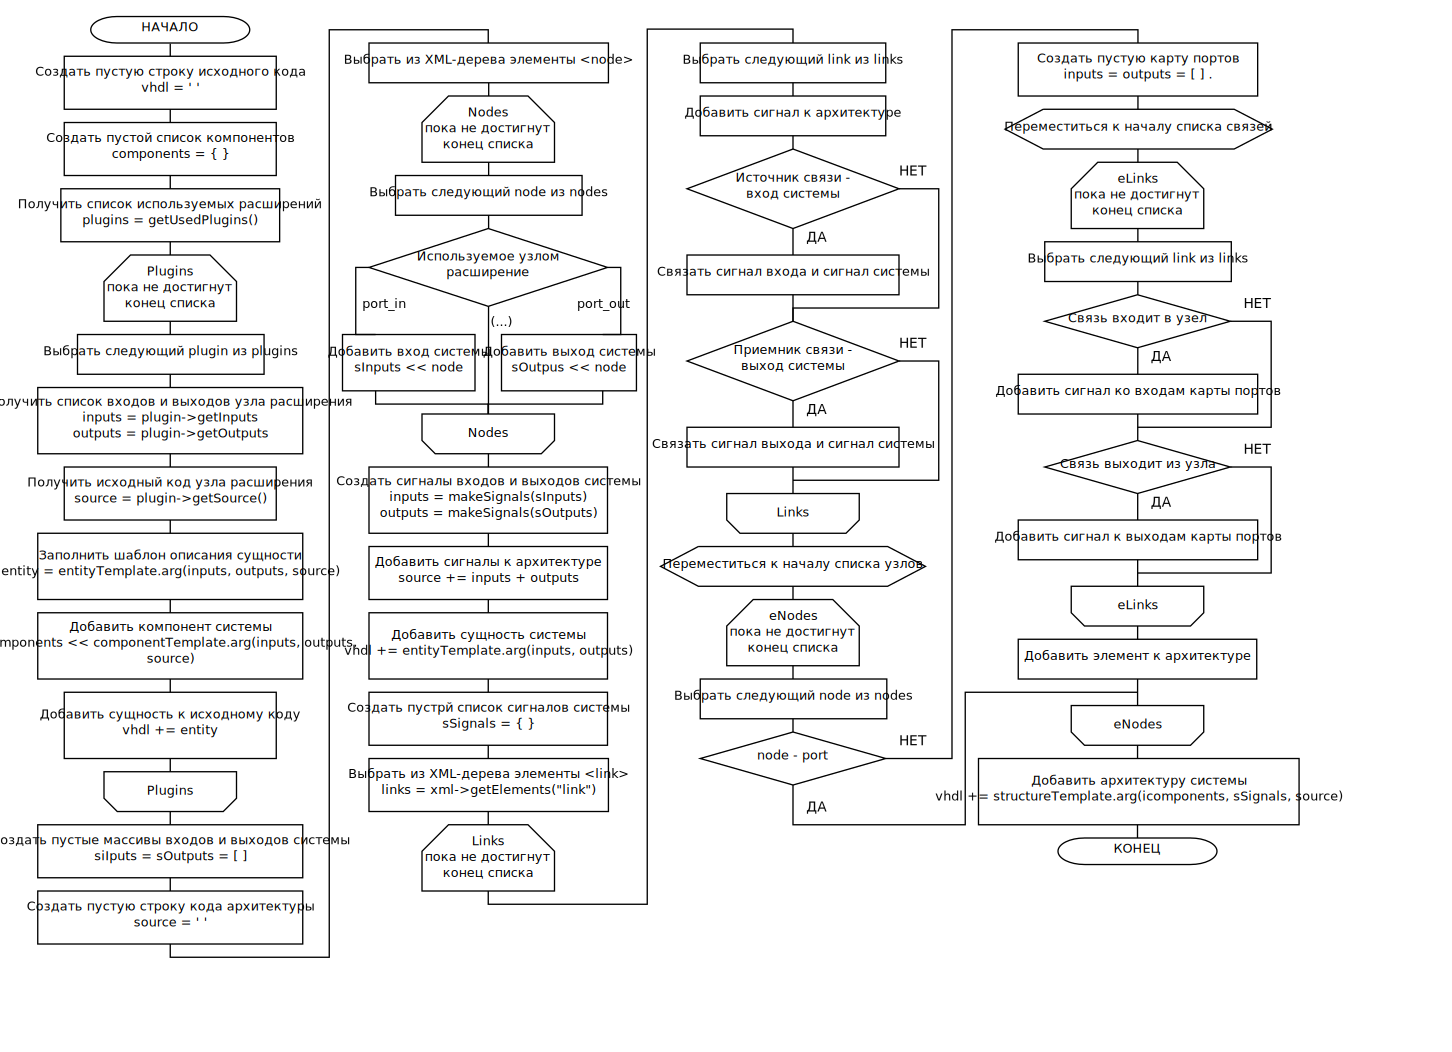
\includegraphics[width=0.95\textwidth]{gui/errors/vhdl.png}
    \caption{Сообщение об ошибке при проверке синтаксиса}
  \end{figure}
\end{itemize}

\newpage
\ESKDthisStyle{formII}
\section{Тестирование системы} \label{sec:testing}
Тестирование функций было проведено по стратегии черного ящика.
Под <<черным ящиком>> понимается объект исследования, внутреннее устройство которого неизвестно.
Черный ящик в кибернетике позволяет изучать поведение систем, то есть их реакций на разнообразные внешние воздействия и в то же время абстрагироваться от их внутреннего устройства.
Манипулируя только лишь со входами и выходами, можно проводить определенные исследования.

Сравнение содержимого документов, выполняемое в данном разделе, проводился с использованием утилиты GNU/diff~--- инструментального средства для построчного сравнения файлов.
diff является утилитой командной строки, обладающей следующим синтаксисом запуска:
\begin{lstlisting}
  diff [ ОПЦИИ  ] [ ФАЙЛЫ  ]
\end{lstlisting}

Среди опций особого внимания заслуживает опция \textbf{-s}: при совпадении файлов ее использование приведет к выводу соответствующего сообщения.

\subsection{Добавление и удаление элементов}
\textbf{Исходные данные:}

Пустой документ.\\

\textbf{Механизм тестирования:}
\begin{enumerate}
  \item Добавить в схему метку.
  \item Сохранить документ, изучить его содержимое.
  \item Добавить в схему два узла.
  \item Сохранить документ, изучить его содержимое.
  \item Добавить в схему связь.
  \item Сохранить документ, изучить его содержимое.
  \item Удалить созданные элементы.
  \item Сохранить документ, изучить его содержимое.
\end{enumerate}

\textbf{Результат:}
\begin{enumerate}
  \item Добавленная метка:
  \begin{lstlisting}[xleftmargin=0cm]
<!DOCTYPE SVE>
<document height="560" width="980">
 <label id="1400577527716" x="0" y="0" text="TEST"/>
</document>
  \end{lstlisting}
  \item Добавленные узлы:
  \begin{lstlisting}[xleftmargin=0cm]
<!DOCTYPE SVE>
<document height="560" width="980">
 <label id="1400577527716" x="0" y="0" text="TEST"/>
 <node id="1400577736807" x="110" plugin="not_gate" y="30"/>
 <node id="1400577743141" x="0" plugin="not_gate" y="30"/>
</document>
  \end{lstlisting}
  \item Добавленная связь:
  \begin{lstlisting}[xleftmargin=0cm]
<!DOCTYPE SVE>
<document height="560" width="980">
 <label id="1400577527716" x="0" y="0" text="TEST"/>
 <node id="1400577736807" x="110" plugin="not_gate" y="30"/>
 <node id="1400577743141" x="0" plugin="not_gate" y="30"/>
 <link last_id="1400577736807" last_connector="0" first_id="1400577743141" id="1400577974692" first_connector="0"/>
</document>
  \end{lstlisting}
  \item Удаление элементов:
  \begin{lstlisting}[xleftmargin=0cm]
<!DOCTYPE SVE>
<document height="560" width="980">
 <label id="1400577527716" x="0" y="0" text="TEST"/>
 <node id="1400577736807" x="110" plugin="not_gate" y="30"/>
 <node id="1400577743141" x="0" plugin="not_gate" y="30"/>
</document>

<!DOCTYPE SVE>
<document height="560" width="980">
 <label id="1400577527716" x="0" y="0" text="TEST"/>
 <node id="1400577736807" x="110" plugin="not_gate" y="30"/>
</document>

<!DOCTYPE SVE>
<document height="560" width="980">
 <label id="1400577527716" x="0" y="0" text="TEST"/>
</document>

<!DOCTYPE SVE>
<document height="560" width="980"/>
  \end{lstlisting}
\end{enumerate}

Как видно, XML-документ последовательно изменялся, наполняясь новыми узлами по мере добавления элементов.
Удаление элементов ведет к удалению узлов из XML-дерева документа.
Можно сделать вывод, что процессы добавления и удаления элементов протекали нормально и без ошибок.


\subsection{Изменение элементов}
\textbf{Исходные данные:}

Проверяемый документ:
\begin{lstlisting}
<!DOCTYPE SVE>
<document height="560" width="980">
 <label id="1400577527716" x="0" y="0" text="TEST"/>
 <node id="1400578932545" x="0" plugin="not_gate" y="30"/>
 <node id="1400578944621" x="140" plugin="and_gate" y="40"/>
 <link last_id="1400578944621" last_connector="0" first_id="1400578932545" id="1400578956357" first_connector="0"/>
</document>
\end{lstlisting}

\textbf{Механизм тестирования:}
\begin{enumerate}
  \item Изменить текст метки.
  \item Переместить один из узлов.
  \item Изменить соединение связи.
  \item Сохранить документ, сравнить его с исходным.
\end{enumerate}

\textbf{Результат:}

\begin{lstlisting}
diff 0.sve 0-change.sve
\end{lstlisting}

Выполнение указанной команды позволит выявить различия в файлах.

\begin{lstlisting}
3c3
<  <label id="1400577527716" x="0" y="0" text="TEST"/>
---
>  <label id="1400577527716" x="0" y="0" text="CHANGE"/>
5,6c5,6
<  <node id="1400578944621" x="140" plugin="and_gate" y="40"/>
<  <link last_id="1400578944621" last_connector="0" first_id="1400578932545" id="1400578956357" first_connector="0"/>
---
>  <node id="1400578944621" x="130" plugin="and_gate" y="150"/>
>  <link last_id="1400578944621" last_connector="1" first_id="1400578932545" id="1400578956357" first_connector="0"/
\end{lstlisting}

Из вывода видно, что файлы различаются тремя строками:
\begin{enumerate}
  \item Метка с текстом <<TEST>> теперь содержит текст <<CHANGE>>.
  \item Узел <<and\_gate>>, ранее имевший координаты (140; 40) теперь имеет координаты (130; 150).
  \item last\_connector связи сменился с <<0>> на <<1>>.
\end{enumerate}

Указанные изменения в документе отразили произошедшие в документе правки, следовательно, процесс изменения элементов работал корректно.

\subsection{Сохранение и загрузка файлов}
\textbf{Исходные данные:}
\begin{figure}[H]
  \centering
  \includegraphics[width=0.6\textwidth]{gui/test/source.png}
  \caption{Проверяемая схема}
  \label{fig:source-test-scheme}
\end{figure}

\textbf{Механизм тестирования:}
\begin{enumerate}
  \item Сохранить схему.
  \item Открыть сохраненный файл.
  \item Сравнить внешний вид схемы с рисунком \ref{fig:source-test-scheme}.
  \item Сохранить схему повторно под другим именем.
  \item Сравнить полученные в результате файлы.
\end{enumerate}

\textbf{Результат:}
\begin{figure}[H]
  \centering
  \includegraphics[width=0.7\textwidth]{gui/test/load-res.png}
  \caption{Загруженная схема}
  \label{fig:load-test-scheme}
\end{figure}

\begin{lstlisting}
diff -s test1.sve test2.sve
\end{lstlisting}

Выполнение указанной команды позволит определить, одинаковы ли файлы.
\begin{lstlisting}
Files test1.sve and test2.sve are identical
\end{lstlisting}

Визуальное изучение схемы и результат построчного сравнения файлов показали, что они идентичны.
Значит, процесс загрузки файлов протекал корректно, сохраняя структуру и содержимое документа.

\subsection{История изменений}
\textbf{Исходные данные:}

Пустой документ.\\

\textbf{Механизм тестирования:}
\begin{enumerate}
  \item Внести в документ изменение и сохранить документ (1).
  \item Внести в документ изменение и сохранить документ (1-change).
  \item Отменить изменение в документе.
  \item Сохранить его под новым именем (2).
  \item Сравнить внешний вид схем до внесения и после отмены изменения.
  \item Сравнить документы (1) и (2).
\end{enumerate}

\textbf{Результат:}
\begin{figure}[H]
  \centering
  \includegraphics[width=1\textwidth]{gui/test/history-1.png}
  \caption{Созданная схема}
  \label{fig:test-hist-1}
\end{figure}

\begin{figure}[H]
  \centering
  \includegraphics[width=1\textwidth]{gui/test/history-1-change.png}
  \caption{Схема со внесенными изменениями}
  \label{fig:test-hist-1-change}
\end{figure}

\begin{figure}[H]
  \centering
  \includegraphics[width=1\textwidth]{gui/test/history-2.png}
  \caption{Схема после отмены изменений}
  \label{fig:test-hist-2}
\end{figure}

Сравнение исходного и измененного файлов:
\begin{lstlisting}
diff -s 1.sve 1-change.sve
\end{lstlisting}

Файлы различаются одной добавленной строкой:
\begin{lstlisting}
4d3
<  <label x="30" id="1400409971081" y="60" text="CHANGE"/>
\end{lstlisting}

Сравнение файлов после отмены изменений:
\begin{lstlisting}
diff -s 1.sve 2.sve
\end{lstlisting}

Файлы идентичны:
\begin{lstlisting}
Files 1.sve and 2.sve are identical
\end{lstlisting}

Очевидно, процесс отмены изменений протекал корректно, сохраняя структуру и содержимое документа.

\subsection{Экспорт схемы в графическом формате}
\textbf{Исходные данные:}
\begin{figure}[H]
  \centering
  \includegraphics[width=1\textwidth]{gui/test/export-1.png}
  \caption{Экспортируемая схема}
  \label{fig:test-export-1}
\end{figure}

\textbf{Механизм тестирования:}
\begin{enumerate}
  \item Экспортировать схему в формате изображения.
  \item Сравнить полученное изображение с отображаемым в программе.
\end{enumerate}

\textbf{Результат:}
\begin{figure}[H]
  \centering
  \includegraphics[width=1\textwidth]{gui/test/export-2.png}
  \caption{Экспортированное изображение}
  \label{fig:test-export-2}
\end{figure}

Сравнение рисунков \ref{fig:test-export-1} и \ref{fig:test-export-2} показало, что процесс экспорта схемы в графическом формате работает корректно.

\subsection{Получение программного описания}
\textbf{Исходные данные:}
\begin{figure}[H]
  \centering
  \includegraphics[width=0.6\textwidth]{gui/test/source.png}
  \caption{Проверяемая схема}
\end{figure}

\textbf{Механизм тестирования:}
\begin{enumerate}
  \item Получить программное описание системы.
  \item Проверить корректность синтаксиса.
  \item Скомпилировать систему.
  \item Запустить полученную систему.
\end{enumerate}

Шаги 2 -- 4 выполнялись с использованием утилиты GHDL, назначение которой описано в пункте \ref{sec:software-structure-components}.\\

\textbf{Результат:}

Полученное программное описание:
\begin{lstlisting}
-- SVE direct export

entity and_gate is
port (
	IN1 : in BIT;
	IN2 : in BIT;
	OUT1 : out BIT);
end entity and_gate;

architecture functional of and_gate is
begin
OUT1 <= IN1 and IN2;
end architecture functional;

entity or_gate is
port (
	IN1 : in BIT;
	IN2 : in BIT;
	OUT1 : out BIT);
end entity or_gate;

architecture functional of or_gate is
begin
OUT1 <= IN1 or IN2;
end architecture functional;

entity not_gate is
port (
	IN1 : in BIT;
	OUT1 : out BIT);
end entity not_gate;

architecture functional of not_gate is
begin
OUT1 <= not IN1;
end architecture functional;

-- SVE entity
entity sve is
port (
	SVEIN1 : in BIT;
	SVEIN2 : in BIT;
	SVEIN3 : in BIT;
	SVEIN4 : in BIT;
	SVEOUT1 : out BIT;
	SVEOUT2 : out BIT);
end entity sve;

architecture structure of sve is
component and_gate is
port (
	IN1 : in BIT;
	IN2 : in BIT;
	OUT1 : out BIT);
end component and_gate;

component or_gate is
port (
	IN1 : in BIT;
	IN2 : in BIT;
	OUT1 : out BIT);
end component or_gate;

component not_gate is
port (
	IN1 : in BIT;
	OUT1 : out BIT);
end component not_gate;

signal SVESIG1: BIT;
signal SVESIG2: BIT;
signal SVESIG3: BIT;
signal SVESIG4: BIT;
signal SVESIG5: BIT;
signal SVESIG6: BIT;
signal SVESIG7: BIT;
signal SVESIG8: BIT;
signal SVESIG9: BIT;

begin
	SVESIG1 <= SVEIN1;
	SVESIG2 <= SVEIN2;
	SVESIG3 <= SVEIN3;
	SVEOUT1 <= SVESIG6;
	SVEOUT2 <= SVESIG8;
	SVESIG9 <= SVEIN4;
	SVESIG7 <= SVESIG6;
	SVENODE4 : and_gate port map (SVESIG1, SVESIG9, SVESIG4);
	SVENODE5 : and_gate port map (SVESIG2, SVESIG3, SVESIG5);
	SVENODE6 : or_gate port map (SVESIG4, SVESIG5, SVESIG6);
	SVENODE8 : not_gate port map (SVESIG7, SVESIG8);
end architecture structure;
\end{lstlisting}

Данный программный код был сохранен в файл sve.vhdl.

Проверка корректности синтаксиса:
\begin{lstlisting}
ghdl -s sve.vhdl
\end{lstlisting}

Выполнение команды не привело к выводу сообщений об ошибках, значит, полученное программное описание синтаксически верно.

Проверка компилируемости системы:
\begin{lstlisting}
ghdl -a sve.vhdl
\end{lstlisting}

Указанная команда была первым шагом компиляции и выполняет анализ системы.
Выполнение ее не привело к выводу сообщений об ошибках, а в результате работы были созданы файлы \textbf{work-obj93.cf} и \textbf{sve.o}.

Первый файл~--- компонентный файл, описывающий структуру конечной системы, второй~--- объектный файл системы.

Следующим шагом было построение системы:
\begin{lstlisting}
ghdl -e sve
\end{lstlisting}

Ошибок также не возникло, был создан файл \textbf{sve}~--- исполняемый файл системы.

Проверка запуска:
\begin{lstlisting}
ghdl -r sve
\end{lstlisting}

Процесс завершился корректно, без сообщений об ошибках.

Можно сделать вывод, что получаемые в результате работы системы программные описания синтаксически корректны и компилируемы.

\newpage
\ESKDthisStyle{formII}
\section{Экономический раздел} \label{sec:economics}
\subsection{Цель дипломного проекта}
Результаты данного дипломного проекта могут быть использованы при обучении студентов в курсе дисциплин <<Цифровые вычислительные устройства и микропроцессорные системы>>, <<Электротехника и электроника>>, <<Цифровая электроника>> и ряду аналогичных.
Введение данной программы позволяет сократить затраты на натурное моделирование, повысить самостоятельность студентов в рамках учебного процесса, уменьшить нагрузку на преподавателей, расширить возможности для дистанционного обучения.

Назначением данного дипломного проекта на предприятии является повышение эффективности процесса обучения.

\subsection{Вид и порядок расчета}
Расчет экономической эффективности проекта производится до начала проектирования и разработки системы.
Это позволяет оценить экономический эффект от внедрения системы.

Порядок расчета:
\begin{itemize}
  \item определение этапов и работ, входящих в общий комплекс работ по созданию программного продукта;
  \item расчет трудоемкости выполнения отдельных этапов и работ и общей трудоемкости разработки;
  \item расчет продолжительности каждой работы;
  \item построение графика разработки программного продукта;
  \item расчет себестоимости разработки;
  \item расчет экономической эффективности от внедрения системы.
\end{itemize}

\subsection{Объем и места внедрения}
Данное приложение планируется ко внедрению на кафедре <<Измерительно-вычислительные комплексы>> Ульяновского государственного технического университета.

\subsection{Достоинства разрабатываемой программы}
\begin{itemize}
  \item Простота: пользовательский интерфейс спроектирован максимально простым и приближенным к виду простых схемных и графических редакторов;
  \item Быстрота внедрения: система, будучи разработанной как независимое приложение, готова ко внедрению на ПЭВМ, удовлетворяющих системным требованиям~--- без необходимости установки дополнительных программных пакетов и комплексов;
  \item Легковесность и платформонезависимость: за счет использования специализированных технологий разработки становится возможным создать решение, обладающее необходимыми показателями производительности и надежности;
  \item Универсальность: полученный в результате работы САПР программный код может быть применен впоследствии в прочих специализированных программных продуктах: визуализаторах, симуляторах работы интегральных схем, а также преобразован для непосредственной загрузки в ПЗУ ПЛИС.
  \item Бесплатность: в отличие от специализированных САПР, представляющих бесплатные версии только для личного индвидуального использования, разрабатываемая система бесплатна и открыта для всех.
\end{itemize}

\subsection{Источники экономии и дохода, источники финансирования}

Необходимо отметить, что разработка ведется на некоммерческой основе в соответствии с принципами и философией создания свободного программного обеспечения: свободой использовать ПО, изучать принципы его функционирования, вносить в него изменения и распространять.
С связи с этим финансирование проекта ведется из личных фондов.

Для объекта внедрения при этом можно выделить следующие факторы экономии:
\begin{itemize}
  \item факт задействования САПР позволяет отказаться от устаревших морально и физически модельных стендов, техническое обслуживание которых затруднено в силу ветхости самих устройств и трудности поиска компонентов для ремонта и замены;
  \item за счет более низких системных требований используемое ПО позволит более эффективно расходовать машинное время во время лабораторных практикумов;
  \item простота освоения ПО позволит не тратить время преподавателей и студентов на переобучение для работы со специализированными конкурентными САПР;
  \item низкие системные требования позволяют использовать ПО на большем количестве аудиторных ЭВМ без необходимости форсированного обновления технопарка;
  \item использование собственной САПР позволит отказаться от приобретения специализированных коммерческих продуктов.
\end{itemize}

\subsubsection{Определение этапов и работ по созданию программного средства}
Процесс разработки программных средств можно разделить на отдельные стадии, каждую из которых можно подразделить на отдельные этапы и подразделы.
Согласно ГОСТ 23501.1-79 регламентируются следующие стадии проведения исследования:
\begin{enumerate}
  \item техническое задание~--- ТЗ (ГОСТ 23501.2-79);
  \item эскизный проект~--- ЭП (ГОСТ 23501.5-80);
  \item технический проект~--- ТП (ГОСТ 23501.6-80);
  \item рабочий проект~--- РП (ГОСТ 23501.11-81);
  \item внедрение~--- ВП (ГОСТ 23501.15-81).
  \item эксплуатация и сопровождение.
\end{enumerate}

Все эти работы выполняются одним исполнителем~--- программистом.
Необходимости привлечения специалистов иных профилей нет.

Содержание основных работ по всем стадиям разработки приведены в таблице \ref{table:schedule}.

\small
\begin{longtable}[h]{|p{0.77\textwidth}|p{0.17\textwidth}|}
  \caption{Содержание основных работ по созданию системы}
  \label{table:schedule}
  \\ \hline
	  \textbf{Наименование работ}   &
	  \textbf{Этап}
	\\ \hline
  \endfirsthead

  \multicolumn{2}{r}{Продолжение таблицы \thetable{}}
  \\ \hline
	  \textbf{Наименование работ}   &
	  \textbf{Этап}
	\\ \hline
  \endhead

  Постановка задачи                                                     &
  \\
  Сбор материалов и анализ существующих разработок                      &
  \\
  Подбор литературы                                                     & ТЗ
  \\
  Определение требований к системе                                      &
  \\
  Определение стадий, этапов и сроков разработки САПР                   &
  \\
  Анализ схожих программных средств                                     &
  \\ \hline

  Разработка функциональной схемы программы     &
  \\
  Разработка структуры программы по подсистемам & ЭП
  \\
  Документирование                              &
  \\ \hline

  Выбор инструментальных средств                             &
  \\
  Определение форматов хранения данных                       & ТП
  \\
  Определение требований к аппаратному обеспечению &
  \\ \hline

  Программирование                                     &
  \\
  Тестирование и отладка                               &
  \\
  Разработка программной документации                  & РП
  \\
  Согласование и утверждение работоспособности системы &
  \\
  Опытная эксплуатация                                 &
  \\ \hline

  Анализ данных, полученных в результате эксплуатации             & ВП
  \\
  Корректировка технической документации по результатам испытаний &
  \\ \hline
\end{longtable}
\normalsize



\subsubsection{Расчет трудоемкости и продолжительности работ}
Трудоемкость работ по созданию САПР на каждой стадии определяется в пунктах \ref{sec:money-1} и \ref{sec:money-2}.

Трудоемкость выполнения работ оценивается как суммарная трудоемкость выполнения отдельных этапов и работ.
Эти показатели определяются на основе экспертных оценок в человеко-днях~--- подобная оценка носит вероятностный характер, поскольку зависит от множества трудноопределимых и взаимновлияющих друг на друга факторов.

Трудоемкость каждого вида работ определяется по формуле:
\begin{equation}\label{eq:ec-1}
  T_i = {{3 \cdot T_{min} + 2 \cdot T_{max}} \over {5}},
\end{equation}
\begin{ESKDexplanation}
  \item[где ] $T_{min}$~--- минимально возможная трудоемкость выполнения отдельного вида работ;
  \item $T_{max}$~--- максимально возможная трудоемкость выполнения отдельного вида работ.
\end{ESKDexplanation}

Продолжительность каждого вида работ в календарных днях ($t_i$) определяется в днях по формуле:
\begin{equation}\label{eq:ec-2}
  t_i = {{T_i} \over {N}} \cdot K,
\end{equation}
  \begin{ESKDexplanation}
    \item[где ] $T_i$~--- трудоемкость работ, человек-дней;
    \item $N$~--- численность исполнителей, человек;
    \item $K$~--- коэффициент, учитывающий выходные и праздничные дни:
    \begin{equation}
      K = {K_{cal} \over K_w},
    \end{equation}
    \begin{ESKDexplanation}
      \item[где ] $K_{cal}$~--- число календарных дней;
      \item $K_w$~--- рабочие дни;
    \end{ESKDexplanation}
  \end{ESKDexplanation}

Согласно производственному и налоговому календарю на 2014 год \cite{work-calendar}, количество рабочих дней составляет 247 дней, таким образом: $K = 1,4$.

Полный список видов и этапов работ по созданию ПО, экспертные оценки и расчетные величины их трудоемкости, а также продолжительность каждого вида работ, рассчитанные по формулам (\ref{eq:ec-1}) и (\ref{eq:ec-2}), представлены в таблице \ref{table:wip}.

\small
\begin{longtable}[h]{|p{0.03\textwidth}|p{0.6\textwidth}|p{0.05\textwidth}|p{0.05\textwidth}|p{0.03\textwidth}|p{0.03\textwidth}|p{0.03\textwidth}|}
  \caption{Расчет трудоемкости и продолжительности работ по созданию ПО}
  \label{table:wip}
  \\ \hline
    \multirow{2}{*}{№} & \multirow{2}{*}{Стадии разработки} & \multicolumn{3}{p{0.13\textwidth}|}{\rotatebox[origin=c]{90}{Трудоемкость, чел.дни}} & \rotatebox[origin=c]{90}{Количество работников, чел}. & \rotatebox[origin=c]{90}{~~Продолжительность работы, дни~~} \\ \cline{3-7}
                       &                                    & $T_{min}$     & $T_{max}$     & $T_i$                                                & $N$                                                   & $t_i$                                                     \\ \hline
    \textbf{1}         & \textbf{2}                         & \textbf{3}    & \textbf{4}    & \textbf{5}                                           & \textbf{6}                                            & \textbf{7}
  \\ \hline
  \endfirsthead

  \multicolumn{7}{r}{Продолжение таблицы \thetable{}}
  \\ \hline
	  \textbf{1} & \textbf{2} & \textbf{3} & \textbf{4} & \textbf{5} & \textbf{6} & \textbf{7}
	\\ \hline
  \endhead

  \multicolumn{7}{|c|}{Техническое задание} \\ \hline
  1 & Постановка задачи & 1 & 1 & 1 & 1 & 1,5 \\ \hline
  2 & Сбор материалов и анализ существующих разработок & 2 & 3 & 2 & 1 & 3 \\ \hline
  3 & Подбор литературы & 2 & 3 & 2 & 1 & 3 \\ \hline
  4 & Определение требований к системе & 3 & 4 & 3 & 1 & 4,5 \\ \hline
  5 & Определение стадий, этапов и сроков разработки САПР & 2 & 3 & 2 & 1 & 3 \\ \hline
  \multicolumn{7}{|c|}{Эскизный проект} \\ \hline
  6 & Анализ схожих программных средств & 5 & 6 & 5 & 1 & 7,5 \\ \hline
  7 & Разработка функциональной схемы программы & 10 & 15 & 12 & 1 & 18 \\ \hline
  8 & Разработка структуры программы по подсистемам & 4 & 6 & 5 & 1 & 7,5 \\ \hline
  9 & Документирование & 2 & 3 & 2 & 1 & 3 \\ \hline
  \multicolumn{7}{|c|}{Технический проект} \\ \hline
  10 & Выбор инструментальных средств & 1 & 1 & 1 & 1 & 1,5 \\ \hline
  11 & Определение форматов хранения данных & 2 & 3 & 2 & 1 & 3 \\ \hline
  12 & Определение требований к аппаратному обеспечению & 1 & 2 & 1 & 1 & 1,5 \\ \hline
  \multicolumn{7}{|c|}{Рабочий проект} \\ \hline
  13 & Программирование & 20 & 50 & 32 & 1 & 48 \\ \hline
  14 & Тестирование и отладка & 10 & 15 & 12 & 1 & 18 \\ \hline
  15 & Разработка программной документации & 5 & 7 & 6 & 1 & 9 \\ \hline
  16 & Согласование и утверждение работоспособности системы & 3 & 5 & 4 & 1 & 6 \\ \hline
  \multicolumn{7}{|c|}{Внедрение} \\ \hline
  17 & Опытная эксплуатация & 7 & 14 & 10 & 1 & 15 \\ \hline
  18 & Анализ данных, полученных в результате эксплуатации & 3 & 4 & 3 & 1 & 4,5 \\ \hline
  19 & Корректировка технической документации по результатам испытаний & 2 & 3 & 2 & 1 & 3 \\ \hline
     & \textbf{Общая трудоемкость разработки} & & 107 & & & \\ \hline
\end{longtable}
\normalsize


Таким образом, общая продолжительность проведения работ составит 107 рабочих дней, при последовательном выполнении всех вышеозначенных в таблице \ref{table:wip} этапов работы

\subsubsection{Построение графика разработки программного продукта}
В качестве инструмента планирования работ используем диаграмму Ганта.

Диаграмма Ганта состоит из полос, ориентированных вдоль оси времени.
Каждая полоса на диаграмме представляет отдельную задачу в составе проекта, ее концы~--- моменты начала и завершения работы, ее протяженность~--- длительность работы.
Вертикальной осью диаграммы служит перечень задач.
Кроме того, на диаграмме могут быть отмечены совокупные задачи, проценты завершения, указатели последовательности и зависимости работ, метки ключевых моментов (вехи), метка текущего момента времени <<Сегодня>> и др.

\begin{figure}[H]
  \centering
  \includegraphics[width=0.98\textwidth]{diagrams/gantt.png}
  \caption{Диаграмма Ганта работы над проектом}
\end{figure}

\subsection{Расчет затрат на разработку} \label{sec:money-1}
\subsubsection{Расчет затрат на разработку программной системы}

Сметная стоимость проектирования и внедрения программы включает в себя следующие затраты, определяемые по формуле:
\begin{equation}
  C = C_{main} + C_{add} + C_{soc} + C_{mat} + C_{mach} + C_{n},
\end{equation}
\begin{ESKDexplanation}
  \item[где ] $C$~--- стоимость разработки ПО, руб.;
  \item $C_{main}$~--- основная заработная плата исполнителей, руб.;
  \item $C_{add}$~--- дополнительная заработная плата исполнителей, учитывающая потери времени на отпуска, руб.;
  \item $C_{soc}$~--- отчисления на социальные нужды, руб.;
  \item $C_{mat}$~--- затраты на используемые материалы, руб.;
  \item $C_{mach}$~--- затраты на  машинное время, руб.;
  \item $C_{n}$~--- накладные расходы включают затраты на управление, уборку, ремонт, электроэнергию, отопление и др., руб.
\end{ESKDexplanation}

Основная заработная плата исполнителей определяется по формуле:
\begin{equation}
  C_{main} = C_{a} \cdot T,
\end{equation}
\begin{ESKDexplanation}
  \item[где ] $С_{main}$~--- заработная плата исполнителей (руб.);
  \item $C_{a}$~--- средняя дневная оплата труда работника организации-разработчика программного продукта (1000 руб./чел.дн.);
  \item $T$ ~--- трудоемкость разработки программного продукта (чел.дн.).
\end{ESKDexplanation}

\begin{table}[H]
  \caption{Расчет основной заработной платы}
  \begin{tabular}{|p{0.18\textwidth}|p{0.15\textwidth}|p{0.15\textwidth}|p{0.2\textwidth}|p{0.2\textwidth}|}
  \hline
    Исполнитель & Оклад,\newline руб/мес. & Оклад, руб./дн. & Трудоемкость, чел.-дн. & Сумма, руб.
  \\ \hline
    Программист & 21000                   & 1000            & 107                    & 107000
  \\ \hline
    \multicolumn{4}{|c|}{Основная заработная плата исполнителя $C_{main}$}           & 107000
  \\ \hline
  \end{tabular}
\end{table}

Дополнительная заработная плата исполнителей, учитывающая потери времени на отпуска и болезни (принимается в среднем 15\% от основной заработной платы):

$C_{add} = 0,15 \cdot 107000 = 16050 (\fc{руб.})$

Отчисления на социальные нужды состоят из единого социального налога (ЕСН) и обязательного страхования от несчастных случаев и профессиональных заболеваний. ЕСН включает в себя отчисления во все внебюджетные фонды, в том числе пенсионный, обязательного медицинского страхования, социального страхования. Ставки налогов и их распределение определяются статьей 241 НК РФ.

Ставка налога рассчитывается, исходя из зарплаты сотрудника, при этом действует регрессивная шкала: чем больше зарплата, тем меньше налог.

Обычный размер ставки~--- для наемного работника, имеющего годовой доход менее 624 тыс. руб.~--- составляет 30\%. Типичный пример распределения этих денег для такого работника выглядит так:
\begin{itemize}
  \item Пенсионный фонд Российской Федерации~--- 22\%;
  \item Фонд социального страхования Российской Федерации~--- 2,9\%;
  \item Федеральный фонд обязательного медицинского страхования~--- 5,1\%.
\end{itemize}

Обязательное страхование от несчастных случаев на производстве и профессиональных заболеваний составляет 0,2\%.
Отчисления на социальные нужды рассчитываются относительно выплаченной заработной платы (суммы основной и дополнительной заработной платы) и составляют 30,2\%:

$C_{soc} = 0,302 \cdot (107000 + 16050) = 37161 (\fc{руб.})$

К затратам на используемые материалы относят затраты на магнитные носители данных, бумагу, канцтовары и др.
Затраты по ним определяются по экспертным оценкам.

\begin{table}[H]
  \caption{Расчет стоимости материалов}
  \begin{tabular}{|p{0.535\textwidth}|l|l|}
  \hline
    Материалы             & Количество, шт. & Стоимость, руб.
  \\ \hline
    Бумага писчая, пачек  & 2               & 400
  \\ \hline
    CD-диск               & 10              & 100
  \\ \hline
    Другие канцтовары     &~---             & 500
  \\ \hline
    \multicolumn{2}{|c|}{Общая стоимость материалов $C_{mat}$} & 1000
  \\ \hline
  \end{tabular}
\end{table}

Затраты на машинное время, необходимое для разработки ПО определяют как расходы на приобретение и подготовку материалов научно-технической информации.

Расчет затрат на машинное время осуществляется по формуле:
\begin{equation}
  C_{mach} = P_{mach} \cdot T ,
\end{equation}
\begin{ESKDexplanation}
  \item[где ] $P_{mach}$~--- себестоимость одного часа машинного времени, включающая в себя амортизацию технических средств, затраты на техническое обслуживание и стоимость электроэнергии;
  \item $T$~--- машинное время, используемое для проведение работ.
\end{ESKDexplanation}

Стоимость машинного дня принимается равным исходя из стоимости используемой ЭВМ.
Ноутбук ASUS X550VC принимается равным  22000 руб.
Норма амортизации 3 года, затраты на ремонт отсутствуют~--- в течении всего срока эксплуатации действует гарантия производителя.

Потребление подобного комплекта оборудования принимается равным 80 Вт/час.
При  стоимости 1 кВт$\cdot$ч согласно тарифам на электроэнергию в Ульяновске и Ульяновской области на 2014 год 2,85 руб., получаем

$P_{mach} = 6,84 (\fc{руб/час.})$

Необходимое количество машинного времени для реализации проекта по разработке программы рассчитывается по формуле:
\begin{equation}
  T = T_i \cdot t_{wd} \cdot T_a ,
\end{equation}
\begin{ESKDexplanation}
  \item[где ] $T_i$~--- трудоемкость работ, чел-дн;
  \item $t_{wd}$~--- продолжительность рабочей смены (при пятидневной рабочей неделе $t_{wd}$ = 8 ч);
  \item $T_a$ -- средний коэффициент использования машинного времени (принимается равным 1).
\end{ESKDexplanation}

Тогда

$T = 107 \cdot 8 \cdot 1 = 856 (\fc{ч.})$

Стоимость машинного времени составит:

$C_{mach} = 6,84 \cdot 856 = 5855 (\fc{руб.})$

К статье <<Накладные расходы>> относят расходы, связанные с управлением и организацией работ. Накладные расходы рассчитываются относительно основной заработной платы.
Величина накладных расходов принимается равной 85\% от основной зарплаты исполнителей.

Формула расчета:
\begin{equation}
  C_n = C_{main} \cdot K ,
\end{equation}
\begin{ESKDexplanation}
  \item[где ] $C_n$~--- накладные расходы, руб.;
  \item $C_{main}$~--- основная заработная плата исполнителей, руб.;
  \item $K$~--- коэффициент учета накладных расходов ($K = 0,85$).
\end{ESKDexplanation}

$C_n = 107000 \cdot 0,85 = 90950 (\fc{руб.})$

Результаты расчета затрат на проектирование программного обеспечения сведены в таблице \ref{table:cost-summary}.

\begin{table}[H]
  \caption{Смета затрат на разработку и внедрение программы}
  \label{table:cost-summary}
  \begin{tabular}{|p{0.623\textwidth}|l|l|}
  \hline
    Наименование статей             & Обозначение  & Сумма, руб.
  \\ \hline
    Основная заработная плата       & $C_{main}$   & 107000 \\ \hline
    Дополнительная заработная плата & $C_{add}$    & 16050  \\ \hline
    Отчисления на социальные нужды  & $C_{soc}$    & 37161  \\ \hline
    Материалы                       & $C_{mat}$    & 1000   \\ \hline
    Машинное время                  & $C_{mach}$   & 5855   \\ \hline
    Накладные расходы               & $C_n$        & 90950  \\ \hline
    \textbf{Итого}                  & $C$          & 258016 \\ \hline
  \end{tabular}
\end{table}

Таким образом, себестоимость разработки составляет 258016 руб.

Так как программа разрабатывается для внутреннего пользования и не будет продаваться в другие организации, то необходимость высчитывать ее оптовую и розничную цену отсутствует.

\subsection{Расчет основных технико-экономических показателей и эффективности использования программного продукта} \label{sec:money-2}

Экономический эффект~--- абсолютная величина, характеризующую достигнутые благодаря созданию или совершенствованию ПО дополнительные экономические результаты.

Экономическая эффективность~--- результативность экономической деятельности, экономических программ и мероприятий, характеризуемая отношением полученного экономического эффекта (результата) к затратам факторов (ресурсов), обусловившим получение этого результата.

Определим механизм возникновения экономического эффекта.
На кафедре <<Измерительно-вычислительные комплексы>> в учебном процессе задействованы компьютеры определенной конфигурации.

\begin{table}[H]
  \caption{Конфигурация ЭВМ}\label{table:pc-specs}
  \begin{tabular}{|l|p{0.72\textwidth}|}
    \hline
      \textbf{Компонент} & \textbf{Модель}
    \\ \hline
      Материнская плата  & Asus P5KPL-AM IN/ROEM/SI
    \\ \hline
      Процессор          & Intel(R) Core(TM)2 Duo CPU E7500 @ 2.93GHz (2 CPU)
    \\ \hline
      Модуль памяти      & DDR2 2038 MB RAM
    \\ \hline
      Жесткий диск       & Samsung HDD (320 GB, 7200 RPM, SATA-II)
    \\ \hline
      CD, DVD            &~---
    \\ \hline
      Монитор            & Philips Brilliance 19S
    \\ \hline
      Клавиатура         & Defender Magellan 920S PS/2
    \\ \hline
      Мышь               & Defender Flagman 110B PS/2
    \\ \hline
  \end{tabular}
\end{table}

Система автоматиизированного проектирования <<Altera Quartus II>>, используемая для работы с ПЛИС, обладает определенными системными требованиями.
Произведем соотношение этих показателей.

\begin{table}[H]
  \caption{Системные требования САПР <<Altera Quartus II>>}\label{table:compare-req}
  \begin{tabular}{|p{0.44\textwidth}|l|l|}
  \hline
    \textbf{Показатель}             & \textbf{Текущее значение} & \textbf{Требуемое значение}
  \\ \hline
    Тактовая частота процессора     & 2,9 GHz                   & 3,0 GHz
  \\ \hline
    Количество ядер процессора      & 2                         & 2
  \\ \hline
    Объем оперативной памяти        & 2 Gb                      & 4 Gb
  \\ \hline
  \end{tabular}
\end{table}

Как видно из таблицы \ref{table:compare-req}, для соответствия системным требованиям и обеспечения должной работоспособности улучшению (замене) должны подвергнуться процессор и ОЗУ ЭВМ.
Определим цену подобного улучшения.

Увеличения объема ОЗУ можно достичь путем покупки дополнительных модулей памяти~--- нет необходимости в полной замене существующих устройств.
Используем для улучшения модуль ОЗУ HYUNDAI / HYNIX DDR-II DIMM 2Gb <PC2-6400>.
Среднерыночная цена такого модуля памяти составляет 1010 руб.

Улучшение производительности ЦПУ без его замены невозможна: рассмотрим в качестве замены устройство CPU Intel Core 2 Duo E8400 3.0 GHz.
Среднерыночная цена данного процессора~--- 3863 руб.

Улучшению необходимо подвергнуть 24 ЭВМ.

\begin{equation}
  C_{hardware} = N \cdot (C_{RAM} + C_{CPU} + С_{inst}),
\end{equation}
\begin{ESKDexplanation}
  \item[где ] $C_{hardware}$~--- стоимость улучшения аппаратной части;
  \item $N$~--- количество ЭВМ для улучшения;
  \item $C_{RAM}$~--- среднерыночная цена одного выбранного модуля ОЗУ;
  \item $C_{CPU}$~--- среднерыночная цена одного выбранного ЦПУ;
  \item $C_{inst}$~--- стоимость проведения монтажных работ по установке нового оборудования.
\end{ESKDexplanation}

Работы по замене компонентов будут проводиться в сервисном центре.
Стоимость подобной работы, в виду ее сравнительной простоты, невелика и составляет в среднем 300 рублей.

Таким образом, стоимость улучшения аппаратной части равна:

$C_{hardware} = 24 \cdot (1010 + 3863 + 300) = 124152 (\fc{руб.})$

Будем исходить из предположения, что подобные улучшения не ведут к увеличению затрат на техническое обслуживание.

Несмотря на наличие бесплатных пробных версий <<Altera Quartus II>>, они не могут быть использованы в учебном процессе, так как предназначены исключительно для личного использования и должны быть удалены после истечения испытательного срока.

Стоимость коммерческой лицензии~--- 2995\$ (106670 руб.), она предоставляется на срок в 1 год, после чего должна быть продлена.
Стоимость продления лицензии~--- 2495\$ (88862 руб.), длительность данного продления~--- так же один год.

Таким образом, затраты на покупку САПР определяются следующим образом:

\begin{equation}
  C_{software} = C_{licence} + (N - 1) \cdot C_{renew},
\end{equation}
\begin{ESKDexplanation}
  \item[где ] $C_{software}$~--- стоимость покупки и обновления САПР;
  \item $C_{licence}$~--- стоимость покупки САПР;
  \item $N$~--- количество лет эксплуатации САПР;
  \item $C_{renew}$~--- стоимость обновления лицензии.
\end{ESKDexplanation}

Суммарные затраты на аппаратные улучшения и покупку САПР:

\begin{equation}
  C = C_{hardware} + C_{software},
\end{equation}
\begin{ESKDexplanation}
  \item[где ] $C$~--- суммарные затраты;
  \item $C_{hardware}$~--- стоимость аппаратных улучшений;
  \item $C_{software}$~--- стоимость покупки и обновления САПР.
\end{ESKDexplanation}

$C = 124512 + 106670 = 230822 (\fc{руб.})$

Разработка собственной системы, как видно из таблицы \ref{table:cost-summary}, обходится в 258016 рублей~--- таким образом, система покажет свою экономическую выгодность уже после первого года внедрения.
Ее использование позволит отказаться от аппаратного улучшения имеющихся ЭВМ и покупки дорогостоящих специализированных САПР.

Таким образом, можно сделать вывод, что разработка собственной системы экономически целесообразна, оправдана и выгодна.
Использование разрабатываемой программы позволяет намного облегчить работу студентов, сократить нагрузку на преподавателей и ведет к значительному сокращению денежных затрат по указанным ранее пунктам.

\newpage
\ESKDthisStyle{formII}
\section{Безопасность и экологичность проекта} \label{sec:safety}
\input{./safety.tex}

\newpage
\ESKDthisStyle{formII}
\section*{Заключение}\addcontentsline{toc}{section}{Заключение}
Процесс разработки SVE был достаточно трудоемок, была проделана значительная работа по разработке архитектуры системы, которая бы позволила не только решить поставленные задачи, но и разделить графический интерфейс и непосредственную работу с документом.
В результате подобного разделения было получено гибкое решение, которое может быть с легкостью встроено в сторонние продукты, а внесение изменений в интерфейс и ядро системы может проводиться независимо.

Значительные усилия были затрачены на проектирование структуры документов с целью, во-первых, обеспечения полноты и неизбыточности отражаемой в документе информации, во-вторых, возможности реализации простых и эффективных механизмов внесения изменений, в-третьих, исключения дополнительных преобразований для обработки информации.
Полученное решение позволяет выполнять рабочие операции и чтение и запись документа без промежуточных форматов~--- исключительно путем оперирования с XML-деревом.

С поставленными задачами система справляется в полной мере, реализуя все заявленные функции.

Хотя система создавалась для использования в учебном процессе, ее можно рассматривать как универсальное решение.
VHDL, выбранный в качестве языка экспорта, позволяет использовать результаты работы программы как в рассмотренных в пункте \ref{sec:characteristics:analogue} аналогичных САПР, так и в отдельных продуктах:
\begin{itemize}
  \item системах для синтеза схем по описанию;
  \item виртуальных измерительных приборах;
  \item симуляторах протекания процессов в системе;
  \item компиляторах программ для ПЗУ ПЛИС.
\end{itemize}

Созданная система имеет дальнейшие перспективы для развития и совершенствования.
Значительно облегчить процесс использования системы может разработка дополнительного компонента, нацеленного на конструирование пользовательских расширений --- сейчас создание расширений ведется в ручном режиме, что может быть затруднительно для пользователя.

К недостаткам системы можно отнести ограниченные возможности встроенного редактора программного кода, обеспечивающего лишь базовую подсветку синтаксиса языка VHDL.
Данный недостаток устаним за счет привлечения сторонних программных решений --- таковым, например, может стать компонент для редактирования исходных кодов <<Scintilla>>.

<<Scintilla>> предоставляет ряд возможностей:
\begin{itemize}
  \item Сворачивание структурных блоков текста (классов, функций, циклов).
  \item Автоматическая установка отступов.
  \item Подсветка парных или непарных (незакрытых) скобок.
  \item Автоматическое завершение используемых в файле имен типов, функций, переменных.
  \item Всплывающие подсказки о параметрах функций.
\end{itemize}

Использование <<Scintilla>> позволит добиться более совершенного отображения получаемого программного кода и превращения средства просмотра в мощный инструмент разработки.

Дальнейшую работу над системой планируется вести в следующем направлении:
\begin{enumerate}
  \item внедрить разработанную версию системы в учебный процесс;
  \item провести первое пользовательское тестирование с целью выявления пожеланий пользователей;
  \item выпустить новую версию системы с учетом результатов пользовательского тестирования;
  \item оптимизировать процесс получения программного описания;
  \item внести изменения в пользовательский интерфейс, расширяющий возможности проектирования схем.
\end{enumerate}

\newpage
\ESKDthisStyle{formII}
\renewcommand\refname{Список использованных источников}
\begin{thebibliography}{0}
\bibitem{maxfield} Максфилд, К. Проектирование на ПЛИС. Курс молодого бойца / К. Максфилд. -- М. : Додэка-XXI, 2007. -- 408 с.
\bibitem{popov} Попов, А. Ю. Проектирование цифровых устройств с использованием ПЛИС / А. Ю. Попов. -- М. : Изд-во МГТУ им. Н. Э. Баумана, 2009. -- 80 с.
\bibitem{butaev} Проектирование цифровых устройств на программируемых логических интегральных схемах / М. М. Бутаев [и др.]. -- Пенза : Изд-во Пенз. гос. техн. ун-та, 1996. -- 65 с.
\bibitem{ugryumov} Угрюмов, Е. П. Цифровая схемотехника / Е. П. Угрюмов. -- СПб. : БХВ-Петербург, 2004. -- 528 с.
\bibitem{bibilo} Бибило, П. Н. Основы языка VHDL / П. Н. Бибило. -- 3-е изд, перераб. -- М. : Издательство ЛКИ, 2007. -- 328 с.
\bibitem{li} Ли, К. Основы САПР / К. Ли. -- СПб. : Питер, 2004. -- 560 с.
\bibitem{quartus} Documentation: Quatus II Development Software. -- Режим доступа: \url{http://www.altera.com/literature/lit-qts.jsp}, свободный. -- Загл. с экрана.
\bibitem{ise} ISE Design Suite. -- Режим доступа: \url{http://www.xilinx.com/products/design-tools/ise-design-suite/}, свободный. -- Загл. с экрана.
\bibitem{work-calendar} Производственный и налоговый календарь для бухгалтера на 2014 год. -- Режим доступа: \url{http://www.ib.ru/law/2290}, свободный. -- Загл. с экрана.
\bibitem{about-qt} Qt 5.3 Released | Qt Project. -- Режим доступа: \url{http://qt-project.org/qt5/qt53}, свободный. -- Загл. с экрана.
\bibitem{qt} All Classes | Documentation | Qt Project. -- Режим доступа: \url{http://qt-project.org/doc/qt-5/classes.html}, свободный. -- Загл. с экрана.
\bibitem{qt-creator} Qt Creator 3.1 | Documentation | Qt Project. -- Режим доступа: \url{http://qt-project.org/doc/qtcreator-3.1/index.html}, свободный. -- Загл. с экрана.
\end{thebibliography}

\newpage
\ESKDthisStyle{formII}
\section*{Приложения}\addcontentsline{toc}{section}{Приложения}
\setcounter{appendix}{0}
\rightappendix{Функциональное моделирование}
\begin{figure}[H]
  \centering
  \includegraphics[width=1.0\textwidth]{diagrams/idef/a1-b.png}
  \caption{Декомпозиция процесса <<Запустить SVE>>}
\end{figure}

\begin{figure}[H]
  \centering
  \includegraphics[width=1.0\textwidth]{diagrams/idef/a11-b.png}
  \caption{Декомпозиция процесса <<Загрузить инструменты>>}
  \label{fig:load-plugins}
\end{figure}

\begin{figure}[H]
  \centering
  \includegraphics[width=1.0\textwidth]{diagrams/idef/a13-b.png}
  \caption{Декомпозиция процесса <<Загрузить схему>>}
  \label{fig:load-scheme}
\end{figure}

\begin{figure}[H]
  \centering
  \includegraphics[width=1.0\textwidth]{diagrams/idef/a3-b.png}
  \caption{Декомпозиция процесса <<Получить результат работы>>}
\end{figure}

\begin{figure}[H]
  \centering
  \includegraphics[width=1.0\textwidth]{diagrams/idef/a31-b.png}
  \caption{Декомпозиция процесса <<Сохранить схему>>}
  \label{fig:save-scheme}
\end{figure}

\begin{figure}[H]
  \centering
  \includegraphics[width=1.0\textwidth]{diagrams/idef/a32-b.png}
  \caption{Декомпозиция процесса <<Экспортировать изображение>>}
\end{figure}

\begin{figure}[H]
  \centering
  \includegraphics[width=1.0\textwidth]{diagrams/idef/a33-b.png}
  \caption{Декомпозиция процесса <<Экспортировать программный код>>}
  \label{fig:export-vhdl}
\end{figure}

\newpage
\rightappendix{Описание программных модулей}
\renewcommand{\thesubsubsection}{\Asbuk{appendix}.\arabic{subsubsection}}
\setcounter{subsection}{0}
\subsubsection*{Программный модуль <<main>>}
Объем: 30 строк

\small
\singlespacing
\begin{longtable}[h]{|p{0.04\textwidth}|p{0.35\textwidth}|p{0.53\textwidth}|}
  \caption{Спецификация модуля <<main>>}
	\\ \hline
	  \textbf{\No}                  &
	  \textbf{Название и тип элемента}  &
	  \textbf{Описание}
	\\ \hline
  \endfirsthead

  \multicolumn{3}{r}{Продолжение таблицы \thetable{}}
  \\ \hline
	  \textbf{\No}                  &
	  \textbf{Название и тип элемента}  &
	  \textbf{Описание}
	\\ \hline
  \endhead

  \multicolumn{3}{|c|}{\textbf{Глобальные переменные}} \\
  \hline
  1 & QSettings settings & Настройки системы \\ \hline
  2 & QApplication a & Экземпляр приложения \\ \hline
  3 & MainWindow w & Главное окно программы \\ \hline

  \multicolumn{3}{|c|}{\textbf{Подпрограммы}} \\
  \hline
  1 & int main(int argc, char *argv[]) &
    \uline{Параметры:}
    \begin{itemize}[nolistsep,label=,leftmargin=0cm]
      \item int argc~--- количество аргументов командой строки
      \item int argv~--- аргументы командной строки
    \end{itemize}
    \uline{Возвращаемое значение:}
    \begin{itemize}[nolistsep,label=,leftmargin=0cm]
      \item 0, если приложение завершилось успешно
    \end{itemize}
  \\ \hline
\end{longtable}
\normalsize
\onehalfspacing


\subsubsection*{Программный модуль <<MainWindow>>}
Объем: 150 строк

\small
\singlespacing
\begin{longtable}[h]{|p{0.04\textwidth}|p{0.35\textwidth}|p{0.53\textwidth}|}
  \caption{Спецификация модуля <<MainWindow>>}
	\\ \hline
	  \textbf{\No}                  &
	  \textbf{Название и тип элемента}  &
	  \textbf{Описание}
	\\ \hline
  \endfirsthead

  \multicolumn{3}{r}{Продолжение таблицы \thetable{}}
  \\ \hline
	  \textbf{\No}                  &
	  \textbf{Название и тип элемента}  &
	  \textbf{Описание}
	\\ \hline
  \endhead

  \multicolumn{3}{|c|}{\textbf{Классы}} \\
  \hline
  1 & class MainWindow : public QMainWindow & Класс главного окна. \\ \hline
\end{longtable}
\normalsize
\onehalfspacing


\small
\singlespacing
\begin{longtable}[h]{|p{0.04\textwidth}|p{0.35\textwidth}|p{0.53\textwidth}|}
  \caption{Спецификация класса <<MainWindow>>}
	\\ \hline
	  \textbf{\No}                  &
	  \textbf{Название и тип элемента}  &
	  \textbf{Описание}
	\\ \hline
  \endfirsthead

  \multicolumn{3}{r}{Продолжение таблицы \thetable{}}
  \\ \hline
	  \textbf{\No}                  &
	  \textbf{Название и тип элемента}  &
	  \textbf{Описание}
	\\ \hline
  \endhead

  \multicolumn{3}{|c|}{\textbf{Поля}} \\
  \hline
  1 & Document *activeDocument; & Текущий документ. \\ \hline
  2 & DocWindow *activeWindow; & Текущее окно документа. \\ \hline
  3 & QSettings *settings; & Настройки документа. \\ \hline
  4 & QList<Plugin *> plugins; & Доступные расширения. \\ \hline
  5 & Ui::MainWindow *ui; & Объект формы. \\ \hline
  6 & QMdiArea *mdiArea; & Многодокументная область. \\ \hline

  \multicolumn{3}{|c|}{\textbf{Методы}} \\
  \hline
  1 & explicit MainWindow(QWidget *parent = 0); &
    Конструктор.\newline
    \uline{Параметры:}
    \begin{itemize}[nolistsep,label=,leftmargin=0cm]
      \item QWidget *parent~--- родительский виджет
    \end{itemize}\\ \hline
  2 & \textasciitilde MainWindow(); & Деструктор. \\ \hline
  3 & void initPluginsToolbar(); & Выносит кнопки расширений на панель быстрого запуска. \\ \hline
  4 & void loadPlugins(); & Просматривает папку, указанную в настройках, на наличие расширений, заносит их в QList plugins. \\ \hline
  5 & void disconnectSlots(); & Отключает обработчики событий от текущего документа. \\ \hline
  6 & void connectSlots(); & Подключает обработчики событий к активному документу. \\ \hline
  7 & void createDocument(); & Обработчик события <<Файл \rarr Создать>> главного меню. Создает новое окно документа, добавляет в него документ, переключает контекст. \\ \hline
  8 & void setActiveDocument(); & Устанавливает *activeDocument на документ в активном окне. \\ \hline
  9 & void quit(); & Обработчик события <<Файл \rarr Выход>> главного меню. Проверяет открытые документы на наличие изменений, закрывает их, осуществляет выход из приложения. \\ \hline
  10 & void load(); & Обработчик события <<Файл \rarr Открыть>> главного меню. Создает окно для документа. Передает управление окну документа. \\ \hline
  11 & void showPluginListWindow(); & Обработчик события <<Настройка \rarr Расширения>> главного меню. Создает и показывает окно управления расширениями. \\ \hline
  12 & void findPlugin(); & Обработчик события нажатия на кнопку расширения в боковой панели. Выбирает расширение из plugins и передает управление активному документу. \\ \hline
  13 & void showPreferencesDialog(); & Обработчик события <<Настройка \rarr Параметры>> главного меню. Создает и показывает окно управления параметрами программы. \\ \hline
  14 & void closeEvent(QCloseEvent *); & Обработчик события закрытия программы. Предотвращает стандартное поведение и передает управление в метод quit(). \\ \hline
\end{longtable}
\normalsize
\onehalfspacing


\subsubsection*{Программный модуль <<PluginListWindow>>}
Объем: 80 строк

\small
\singlespacing
\begin{longtable}[h]{|p{0.04\textwidth}|p{0.35\textwidth}|p{0.53\textwidth}|}
  \caption{Спецификация модуля <<PluginListWindow>>}
	\\ \hline
	  \textbf{\No}                  &
	  \textbf{Название и тип элемента}  &
	  \textbf{Описание}
	\\ \hline
  \endfirsthead

  \multicolumn{3}{r}{Продолжение таблицы \thetable{}}
  \\ \hline
	  \textbf{\No}                  &
	  \textbf{Название и тип элемента}  &
	  \textbf{Описание}
	\\ \hline
  \endhead

  \multicolumn{3}{|c|}{\textbf{Перечисления}} \\
  \hline
  1 & enum class LCol &
    Тип колонки.\newline
    \uline{Значения:}
    \begin{itemize}[nolistsep,label=,leftmargin=0cm]
      \item isEnabled = 0~--- колонка <<Включен>>;
      \item pluginName = 1 -- колонка <<Расширение>>;
      \item isOnPanel = 2~--- колонка <<Активен>>;
      \item author = 3~--- колонка <<Автор>>;
      \item description = 4~--- колонка <<Описание>>.
    \end{itemize} \\ \hline

  \multicolumn{3}{|c|}{\textbf{Классы}} \\
  \hline
  1 & class PluginListWindow : public QDialog & Класс окна управления расширениями. \\ \hline
\end{longtable}
\normalsize
\onehalfspacing


\small
\singlespacing
\begin{longtable}[h]{|p{0.04\textwidth}|p{0.35\textwidth}|p{0.53\textwidth}|}
  \caption{Спецификация класса <<PluginListWindow>>}
	\\ \hline
	  \textbf{\No}                  &
	  \textbf{Название и тип элемента}  &
	  \textbf{Описание}
	\\ \hline
  \endfirsthead

  \multicolumn{3}{r}{Продолжение таблицы \thetable{}}
  \\ \hline
	  \textbf{\No}                  &
	  \textbf{Название и тип элемента}  &
	  \textbf{Описание}
	\\ \hline
  \endhead

  \multicolumn{3}{|c|}{\textbf{Поля}} \\
  \hline
  1 & Ui::PluginListWindow *ui; & Объект формы. \\ \hline
  1 & QDir pluginsDir; & Текущий документ. \\ \hline
  3 & QSettings *settings; & Настройки расширений. \\ \hline

  \multicolumn{3}{|c|}{\textbf{Методы}} \\
  \hline
  1 & explicit PluginListWindow(QWidget *parent = 0); &
    Конструктор.\newline
    \uline{Параметры:}
    \begin{itemize}[nolistsep,label=,leftmargin=0cm]
      \item QWidget *parent~--- родительский виджет
    \end{itemize}\\ \hline
  2 & \textasciitilde PluginListWindow() & Деструктор. \\ \hline
  3 & QList<QTreeWidgetItem *> loadPluginsList(); &
    Сканирует pluginsDir на наличие расширений.\newline
    \uline{Возвращаемое значение:}
    \begin{itemize}[nolistsep,label=,leftmargin=0cm]
      \item QList<QTreeWidgetItem *>~--- список расширений и их параметров для вставки в QTreeWidget.
    \end{itemize} \\ \hline
  4 & void refreshList(); & Обновляет список расширений. \\ \hline
  5 & void save(); & Сохраняет настройки расширений. \\ \hline
\end{longtable}
\normalsize
\onehalfspacing


\subsubsection*{Программный модуль <<PreferencesDialog>>}
Объем: 35 строк

\small
\singlespacing
\begin{longtable}[h]{|p{0.04\textwidth}|p{0.35\textwidth}|p{0.53\textwidth}|}
  \caption{Спецификация модуля <<PreferencesDialog>>}
	\\ \hline
	  \textbf{\No}                  &
	  \textbf{Название и тип элемента}  &
	  \textbf{Описание}
	\\ \hline
  \endfirsthead

  \multicolumn{3}{r}{Продолжение таблицы \thetable{}}
  \\ \hline
	  \textbf{\No}                  &
	  \textbf{Название и тип элемента}  &
	  \textbf{Описание}
	\\ \hline
  \endhead


  \multicolumn{3}{|c|}{\textbf{Классы}} \\
  \hline
  1 & class PreferencesDialog : public QDialog & Класс окна управления настройками программы. \\ \hline
\end{longtable}
\normalsize
\onehalfspacing


\small
\singlespacing
\begin{longtable}[h]{|p{0.04\textwidth}|p{0.35\textwidth}|p{0.53\textwidth}|}
  \caption{Спецификация класса <<PreferencesDialog>>}
	\\ \hline
	  \textbf{\No}                  &
	  \textbf{Название и тип элемента}  &
	  \textbf{Описание}
	\\ \hline
  \endfirsthead

  \multicolumn{3}{r}{Продолжение таблицы \thetable{}}
  \\ \hline
	  \textbf{\No}                  &
	  \textbf{Название и тип элемента}  &
	  \textbf{Описание}
	\\ \hline
  \endhead

  \multicolumn{3}{|c|}{\textbf{Поля}} \\
  \hline
  1 & QSettings *settings; & Настройки программы. \\ \hline

  \multicolumn{3}{|c|}{\textbf{Методы}} \\
  \hline
  1 & explicit PreferencesDialog(QWidget *parent = 0); &
    Конструктор.\newline
    \uline{Параметры:}
    \begin{itemize}[nolistsep,label=,leftmargin=0cm]
      \item QWidget *parent~--- родительский виджет
    \end{itemize}\\ \hline
  2 & \textasciitilde PreferencesDialog(); & Деструктор. \\ \hline
  3 & void browsePath(); & Открывает диалог указания папки расширений. \\ \hline
  4 & void saveOptions(); & Сохраняет настроки программы. \\ \hline
\end{longtable}
\normalsize
\onehalfspacing


\subsubsection*{Программный модуль <<DocWindow>>}
Объем: 200 строк

\small
\singlespacing
\begin{longtable}[h]{|p{0.04\textwidth}|p{0.35\textwidth}|p{0.53\textwidth}|}
  \caption{Спецификация модуля <<DocWindow>>}
	\\ \hline
	  \textbf{\No}                  &
	  \textbf{Название и тип элемента}  &
	  \textbf{Описание}
	\\ \hline
  \endfirsthead

  \multicolumn{3}{r}{Продолжение таблицы \thetable{}}
  \\ \hline
	  \textbf{\No}                  &
	  \textbf{Название и тип элемента}  &
	  \textbf{Описание}
	\\ \hline
  \endhead


  \multicolumn{3}{|c|}{\textbf{Классы}} \\
  \hline
  1 & class DocWindow : public QMdiSubWindow & Класс окна (контейнера) документа. \\ \hline
\end{longtable}
\normalsize
\onehalfspacing


\small
\singlespacing
\begin{longtable}[h]{|p{0.04\textwidth}|p{0.35\textwidth}|p{0.53\textwidth}|}
  \caption{Спецификация класса <<DocWindow>>}
	\\ \hline
	  \textbf{\No}                  &
	  \textbf{Название и тип элемента}  &
	  \textbf{Описание}
	\\ \hline
  \endfirsthead

  \multicolumn{3}{r}{Продолжение таблицы \thetable{}}
  \\ \hline
	  \textbf{\No}                  &
	  \textbf{Название и тип элемента}  &
	  \textbf{Описание}
	\\ \hline
  \endhead

  \multicolumn{3}{|c|}{\textbf{Поля}} \\
  \hline
  1 & Document *document; & Связанный документ. \\ \hline
  2 & QStatusBar *statusBar; & Статусная строка родительского окна документа. \\ \hline
  3 & QList<UNode *> linkNodes; & Буферный список узлов для задания связи. \\ \hline

  \multicolumn{3}{|c|}{\textbf{Методы}} \\
  \hline
  1 & explicit DocWindow(QWidget *parent = 0); &
    Конструктор.\newline
    \uline{Параметры:}
    \begin{itemize}[nolistsep,label=,leftmargin=0cm]
      \item QWidget *parent~--- родительский виджет
    \end{itemize}\\ \hline
  2 & \textasciitilde DocWindow(); & Деструктор. \\ \hline
  3 & void setTitle(const QString title); & Задает заголовок окна.\newline
    \uline{Параметры:}
    \begin{itemize}[nolistsep,label=,leftmargin=0cm]
      \item const QString title~--- заголовок
    \end{itemize}\\ \hline
  4 & Document *getDocument(); & \uline{Возвращаемое значение:}
    \begin{itemize}[nolistsep,label=,leftmargin=0cm]
      \item Document*~--- связанный документ
    \end{itemize}\\ \hline\\ \hline
  5 & void addNode(Plugin *plugin); & Добавляет узел выбранного расширения.\newline
    \uline{Параметры:}
    \begin{itemize}[nolistsep,label=,leftmargin=0cm]
      \item Plugin *plugin~--- расширение
    \end{itemize}\\ \hline
  6 & void attachStatusBar(QStatusBar *statusBar); & Регистрирует статусную строку родительского окна для обращений.\newline
    \uline{Параметры:}
    \begin{itemize}[nolistsep,label=,leftmargin=0cm]
      \item QStatusBar *statusBar~--- статусная строка родительского окна
    \end{itemize}\\ \hline
  7 & bool renderNodes(); & Обрабатывает XML-дерево вложенного документа, добавляя виджеты элементов в рабочую область. \\ \hline
  8 & void setStatus(QString text, int timeout); & Устанавливает содержимое статусной строки родительского окна.\newline
    \uline{Параметры:}
    \begin{itemize}[nolistsep,label=,leftmargin=0cm]
      \item QString text~--- текст статусной строки
      \item int timeout~--- время показа сообщения
    \end{itemize}\\ \hline
  9 & void closeEvent(QCloseEvent *closeEvent); & Обработчик события закрытия окна. Выдает предупреждение о несохраненных изменениях.\newline
    \uline{Параметры:}
    \begin{itemize}[nolistsep,label=,leftmargin=0cm]
      \item QCloseEvent *closeEvent~--- событие закрытия
    \end{itemize}\\ \hline
  10 & void setChanged(bool changed); & Устанавливает флаг изменения для документа.\newline
    \uline{Параметры:}
    \begin{itemize}[nolistsep,label=,leftmargin=0cm]
      \item bool changed~--- признак измененности
    \end{itemize}\\ \hline
  11 & void addLabel(); & Показывает диалоговое окно для ввода текста и добавляет в документ ссылку с этим текстом.\\ \hline
  12 & void addNode(); & Обработчик события <<Схема \rarr Добавить узел>>. Показывает диалог выбора расширения для добавления, передает документу название выбранного расширения. \\ \hline
  13 & void addLink(); & Переводит документ в режим добавления метки. \\ \hline
  14 & void save(); & Сохраняет документ под существующим имененем или показывает диалог сохранения файла, сохраняет документ.\\ \hline
  15 & void saveAs(); & Показывает диалог сохранения файла, сохраняет документ.\\ \hline
  16 & bool load(); & Показывает диалог выбора файла, загружает документ из выбранного файла.\\ \hline
  17 & void setLinkNode(UNode *node, uint nodeCounter); & Обработчик события выбора узла. Добавляет узел к списку выбранных или соединяет выбранные узлы связью.\newline
    \uline{Параметры:}
    \begin{itemize}[nolistsep,label=,leftmargin=0cm]
      \item UNode *node~--- выбранный узел
      \item uint nodeCounter~--- счетчик выбранных узлов
    \end{itemize}\\ \hline
  18 & void showOptionsDialog(); & Показывает диалог свойств документа, сохраняет изменения. \\ \hline
  19 & void showSaveImageDialog(); & Показывает диалог сохранения изображения. \\ \hline
  20 & void viewVHDL(); & Запрашивает исходный код документа, показывает окно просмотра VHDL. \\ \hline
\end{longtable}
\normalsize
\onehalfspacing


\subsubsection*{Программный модуль <<AddNodeDialog>>}
Объем: 25 строк

\small
\singlespacing
\begin{longtable}[h]{|p{0.04\textwidth}|p{0.35\textwidth}|p{0.53\textwidth}|}
  \caption{Спецификация модуля <<AddNodeDialog>>}
	\\ \hline
	  \textbf{\No}                  &
	  \textbf{Название и тип элемента}  &
	  \textbf{Описание}
	\\ \hline
  \endfirsthead

  \multicolumn{3}{r}{Продолжение таблицы \thetable{}}
  \\ \hline
	  \textbf{\No}                  &
	  \textbf{Название и тип элемента}  &
	  \textbf{Описание}
	\\ \hline
  \endhead

  \multicolumn{3}{|c|}{\textbf{Классы}} \\
  \hline
  1 & class AddNodeDialog : public QDialog & Класс окна добавления узла из расширения. \\ \hline
\end{longtable}
\normalsize
\onehalfspacing


\small
\singlespacing
\begin{longtable}[h]{|p{0.04\textwidth}|p{0.35\textwidth}|p{0.53\textwidth}|}
  \caption{Спецификация класса <<AddNodeDialog>>}
	\\ \hline
	  \textbf{\No}                  &
	  \textbf{Название и тип элемента}  &
	  \textbf{Описание}
	\\ \hline
  \endfirsthead

  \multicolumn{3}{r}{Продолжение таблицы \thetable{}}
  \\ \hline
	  \textbf{\No}                  &
	  \textbf{Название и тип элемента}  &
	  \textbf{Описание}
	\\ \hline
  \endhead

  \multicolumn{3}{|c|}{\textbf{Поля}} \\
  \hline
  1 & Ui::AddNodeDialog *ui & Объект формы. \\ \hline

  \multicolumn{3}{|c|}{\textbf{Методы}} \\
  \hline
  1 & explicit AddNodeDialog(QWidget *parent = 0); &
    Конструктор.\newline
    \uline{Параметры:}
    \begin{itemize}[nolistsep,label=,leftmargin=0cm]
      \item QWidget *parent~--- родительский виджет
    \end{itemize}\\ \hline
  2 & \textasciitilde AddNodeDialog(); & Деструктор. \\ \hline
  3 & void itemSelected(QString item); & Сигнал, запускаемый при выборе расширения.\newline
    \uline{Параметры:}
    \begin{itemize}[nolistsep,label=,leftmargin=0cm]
      \item QString item~--- название выбранного расширения
    \end{itemize}\\ \hline
  4 & void getSelection(); & Получает текущее выделенное расширение и запускает сигнал itemSelected.\\ \hline
  5 & void unlockAdd(); & Разблокирует кнопку <<Добавить>>.\\ \hline
\end{longtable}
\normalsize
\onehalfspacing


\subsubsection*{Программный модуль <<DocumentOptionsDialog>>}
Объем: 15 строк

\small
\singlespacing
\begin{longtable}[h]{|p{0.04\textwidth}|p{0.35\textwidth}|p{0.53\textwidth}|}
  \caption{Спецификация модуля <<DocumentOptionsDialog>>}
	\\ \hline
	  \textbf{\No}                  &
	  \textbf{Название и тип элемента}  &
	  \textbf{Описание}
	\\ \hline
  \endfirsthead

  \multicolumn{3}{r}{Продолжение таблицы \thetable{}}
  \\ \hline
	  \textbf{\No}                  &
	  \textbf{Название и тип элемента}  &
	  \textbf{Описание}
	\\ \hline
  \endhead

  \multicolumn{3}{|c|}{\textbf{Классы}} \\
  \hline
  1 & class DocumentOptionsDialog : public QDialog & Класс окна свойств документа. \\ \hline
\end{longtable}
\normalsize
\onehalfspacing


\small
\singlespacing
\begin{longtable}[h]{|p{0.04\textwidth}|p{0.35\textwidth}|p{0.53\textwidth}|}
  \caption{Спецификация класса <<DocumentOptionsDialog>>}
	\\ \hline
	  \textbf{\No}                  &
	  \textbf{Название и тип элемента}  &
	  \textbf{Описание}
	\\ \hline
  \endfirsthead

  \multicolumn{3}{r}{Продолжение таблицы \thetable{}}
  \\ \hline
	  \textbf{\No}                  &
	  \textbf{Название и тип элемента}  &
	  \textbf{Описание}
	\\ \hline
  \endhead

  \multicolumn{3}{|c|}{\textbf{Поля}} \\
  \hline
  1 & Ui::DocumentOptionsDialog *ui & Объект формы. \\ \hline

  \multicolumn{3}{|c|}{\textbf{Методы}} \\
  \hline
  1 & explicit DocumentOptionsDialog( QWidget *parent = 0); &
    Конструктор.\newline
    \uline{Параметры:}
    \begin{itemize}[nolistsep,label=,leftmargin=0cm]
      \item QWidget *parent~--- родительский виджет
    \end{itemize}\\ \hline
  2 & \textasciitilde DocumentOptionsDialog(); & Деструктор. \\ \hline
  3 & void setDimensions(QSize size); & Устанавливает значения счетчиков размера рабочей области.\newline
    \uline{Параметры:}
    \begin{itemize}[nolistsep,label=,leftmargin=0cm]
      \item QSize size~--- размер рабочей области
    \end{itemize}\\ \hline
  4 & QSize getDimensions(); & Возвращает введенный размер рабочей области.\newline
    \uline{Возвращаемое значение:}
    \begin{itemize}[nolistsep,label=,leftmargin=0cm]
      \item QSize ~--- размер рабочей области
    \end{itemize}\\ \hline
\end{longtable}
\normalsize
\onehalfspacing


\subsubsection*{Программный модуль <<SourceViewDialog>>}
Объем: 70 строк

\small
\singlespacing
\begin{longtable}[h]{|p{0.04\textwidth}|p{0.35\textwidth}|p{0.53\textwidth}|}
  \caption{Спецификация модуля <<SourceViewDialog>>}
	\\ \hline
	  \textbf{\No}                  &
	  \textbf{Название и тип элемента}  &
	  \textbf{Описание}
	\\ \hline
  \endfirsthead

  \multicolumn{3}{r}{Продолжение таблицы \thetable{}}
  \\ \hline
	  \textbf{\No}                  &
	  \textbf{Название и тип элемента}  &
	  \textbf{Описание}
	\\ \hline
  \endhead

  \multicolumn{3}{|c|}{\textbf{Классы}} \\
  \hline
  1 & class SourceViewDialog : public QDialog & Окно просмотра исходного кода. \\ \hline
\end{longtable}
\normalsize
\onehalfspacing


\small
\singlespacing
\begin{longtable}[h]{|p{0.04\textwidth}|p{0.35\textwidth}|p{0.53\textwidth}|}
  \caption{Спецификация класса <<SourceViewDialog>>}
	\\ \hline
	  \textbf{\No}                  &
	  \textbf{Название и тип элемента}  &
	  \textbf{Описание}
	\\ \hline
  \endfirsthead

  \multicolumn{3}{r}{Продолжение таблицы \thetable{}}
  \\ \hline
	  \textbf{\No}                  &
	  \textbf{Название и тип элемента}  &
	  \textbf{Описание}
	\\ \hline
  \endhead

  \multicolumn{3}{|c|}{\textbf{Поля}} \\
  \hline
  1 & Ui::SourceViewDialog *ui & Объект формы. \\ \hline
  2 & QString htmlTemplate; & Шаблон для страницы исходного кода. \\ \hline
  3 & QString vhdlSource; & Исходный код. \\ \hline
  4 & QWebView *view; & Веб-виджет для просмотра HTML-страниц. \\ \hline
  5 & bool ghdlNotFound; & Признак отсутствия в системе утилиты GHDL. \\ \hline

  \multicolumn{3}{|c|}{\textbf{Методы}} \\
  \hline
  1 & explicit SourceViewDialog(QString vhdlSource = "", QWidget *parent = 0); &
    Конструктор.\newline
    \uline{Параметры:}
    \begin{itemize}[nolistsep,label=,leftmargin=0cm]
      \item QString vhdlSource~--- исходный код
      \item QWidget *parent~--- родительский виджет
    \end{itemize}\\ \hline
  2 & \textasciitilde SourceViewDialog(); & Деструктор. \\ \hline
  3 & void setSource(QString src); & Задает исходный код.\newline
    \uline{Параметры:}
    \begin{itemize}[nolistsep,label=,leftmargin=0cm]
      \item QString src~--- исходный код
    \end{itemize}\\ \hline
  4 & void validate(); & Проверяет исходный код на валидность, выводит сообщения об ошибках в форму. \\ \hline
  5 & void handleError( QProcess::ProcessError); & Обрабатывает ошибки запуска внешнего процесса.\newline
    \uline{Параметры:}
    \begin{itemize}[nolistsep,label=,leftmargin=0cm]
      \item QProcess::ProcessError~--- код ошибки
    \end{itemize}\\ \hline
\end{longtable}
\normalsize
\onehalfspacing


\subsubsection*{Программный модуль <<Document>>}
Объем: 680 строк

\small
\singlespacing
\begin{longtable}[h]{|p{0.04\textwidth}|p{0.35\textwidth}|p{0.53\textwidth}|}
  \caption{Спецификация модуля <<Document>>}
	\\ \hline
	  \textbf{\No}                  &
	  \textbf{Название и тип элемента}  &
	  \textbf{Описание}
	\\ \hline
  \endfirsthead

  \multicolumn{3}{r}{Продолжение таблицы \thetable{}}
  \\ \hline
	  \textbf{\No}                  &
	  \textbf{Название и тип элемента}  &
	  \textbf{Описание}
	\\ \hline
  \endhead

  \multicolumn{3}{|c|}{\textbf{Перечисления}} \\
  \hline
  1 & enum NodeType &
    Тип элемента.\newline
    \uline{Значения:}
    \begin{itemize}[nolistsep,label=,leftmargin=0cm]
      \item Stub = 0~--- заглушка;
      \item Node = 1--- узел;
      \item Label = 2--- метка;
      \item Link  = 3--- связь;
    \end{itemize} \\ \hline
  1 & enum DocumentMode &
    Режим документа.\newline
    \uline{Значения:}
    \begin{itemize}[nolistsep,label=,leftmargin=0cm]
      \item Default = 0~--- стандартный режим;
      \item SelectNode = 1~--- режим выбора узлов;
    \end{itemize} \\ \hline

  \multicolumn{3}{|c|}{\textbf{Классы}} \\
  \hline
  1 & class Document: public QObject & Окно просмотра исходного кода. \\ \hline
\end{longtable}
\normalsize
\onehalfspacing


\small
\singlespacing
\begin{longtable}[h]{|p{0.04\textwidth}|p{0.35\textwidth}|p{0.53\textwidth}|}
  \caption{Спецификация класса <<Document>>}
	\\ \hline
	  \textbf{\No}                  &
	  \textbf{Название и тип элемента}  &
	  \textbf{Описание}
	\\ \hline
  \endfirsthead

  \multicolumn{3}{r}{Продолжение таблицы \thetable{}}
  \\ \hline
	  \textbf{\No}                  &
	  \textbf{Название и тип элемента}  &
	  \textbf{Описание}
	\\ \hline
  \endhead

  \multicolumn{3}{|c|}{\textbf{Поля}} \\
  \hline
  1 & QString title; & Заголовок документа. \\ \hline
  2 & QString filename; & Файл документа. \\ \hline
  3 & QMdiSubWindow *parent; & Вкладка-контейнер. \\ \hline
  4 & QScrollArea *container; & Область прокрутки. \\ \hline
  5 & QFrame *workarea; & Рабочая область. \\ \hline
  6 & QDomDocument *xml; & XML-представление документа. \\ \hline
  7 & bool changed; & Признак изменения. \\ \hline
  8 & DocumentMode mode; & Режим документа. \\ \hline
  9 & QStack<QByteArray> history; & Стек истории изменений. \\ \hline
  10 & QList<Plugin*> plugins; & Список расширений, доступных для использования в документе. \\ \hline
  11 & UNode *activeElement; & Выбранный элемент. \\ \hline
  12 & uint nodeCounter; & Счетчик выбранных узлов. \\ \hline

  \multicolumn{3}{|c|}{\textbf{Методы}} \\
  \hline
  1 & explicit Document(QMdiSubWindow *parent = 0); &
    Конструктор.\newline
    \uline{Параметры:}
    \begin{itemize}[nolistsep,label=,leftmargin=0cm]
      \item QMdiSubWindow *parent~--- контейнер
    \end{itemize}\\ \hline
  2 & \textasciitilde Document(); & Деструктор. \\ \hline
  3 & void altered(bool); & Сигнал, запускаемый при изменении документа.\newline
    \uline{Параметры:}
    \begin{itemize}[nolistsep,label=,leftmargin=0cm]
      \item bool~--- признак изменения документа
    \end{itemize}\\ \hline
  4 & void elementActivated(UNode*, uint); & Сигнал, запускаемый при выборе элемента.\newline
    \uline{Параметры:}
    \begin{itemize}[nolistsep,label=,leftmargin=0cm]
      \item UNode*~--- выбранный элемент
      \item uint~--- количество ранее выбранных элементов
    \end{itemize}\\ \hline
  5 & void  attachToWindow( QMdiSubWindow *parent); & Прикрепляет документ к контейнеру.\newline
    \uline{Параметры:}
    \begin{itemize}[nolistsep,label=,leftmargin=0cm]
      \item QMdiSubWindow *parent~--- контейнер
    \end{itemize}\\ \hline
  6 & QSize getSize(); & Возвращает размер рабочей области.\newline
    \uline{Возвращаемое значение:}
    \begin{itemize}[nolistsep,label=,leftmargin=0cm]
      \item QSize ~--- размер рабочей области
    \end{itemize}\\ \hline
  7 & void  resize(const QSize size); & Задает размер рабочей области.\newline
    \uline{Параметры:}
    \begin{itemize}[nolistsep,label=,leftmargin=0cm]
      \item QSize size~--- размер рабочей области
    \end{itemize}\\ \hline
  8 & void  resize(const int w, const int h); & Задает размер рабочей области.\newline
    \uline{Параметры:}
    \begin{itemize}[nolistsep,label=,leftmargin=0cm]
      \item const int w~--- ширина
      \item const int h~--- высота
    \end{itemize}\\ \hline
  9 & bool isChanged(); & Возвращает признак изменения документа.\newline
    \uline{Возвращаемое значение:}
    \begin{itemize}[nolistsep,label=,leftmargin=0cm]
      \item bool ~--- признак изменения
    \end{itemize}\\ \hline
  10 & void setChanged(bool changed); & Устанавливает признак изменения документа.\newline
    \uline{Параметры:}
    \begin{itemize}[nolistsep,label=,leftmargin=0cm]
      \item bool changed~--- признак изменения
    \end{itemize}\\ \hline
  11 & void addLabel(const QString text,  bool skipHistory = false); & Добавляет виджет метки.\newline
    \uline{Параметры:}
    \begin{itemize}[nolistsep,label=,leftmargin=0cm]
      \item const QString text~--- текст метки
      \item bool skipHistory = false~--- пропустить изменение в истории
    \end{itemize}\\ \hline
  12 & void addLabel(const QDomNode node, bool skipHistory = false); & Добавляет виджет метки.\newline
    \uline{Параметры:}
    \begin{itemize}[nolistsep,label=,leftmargin=0cm]
      \item const QDomNode node~--- XML-узел
      \item bool skipHistory = false~--- пропустить изменение в истории
    \end{itemize}\\ \hline
  13 & void addNode(Plugin *plugin,       bool skipHistory = false); & Добавляет виджет узла.\newline
    \uline{Параметры:}
    \begin{itemize}[nolistsep,label=,leftmargin=0cm]
      \item Plugin *plugin~--- расширение
      \item bool skipHistory = false~--- пропустить изменение в истории
    \end{itemize}\\ \hline
  14 & bool addNode(const QDomNode node,  bool skipHistory = false); & Добавляет виджет узла.\newline
    \uline{Параметры:}
    \begin{itemize}[nolistsep,label=,leftmargin=0cm]
      \item const QDomNode node~--- XML-узел
      \item bool skipHistory = false~--- пропустить изменение в истории
    \end{itemize}\\ \hline
  15 & void addLink(QList<UNode *> elementNodes, QPair<int, int> connectors, bool skipHistory = false); & Добавляет виджет связи.\newline
    \uline{Параметры:}
    \begin{itemize}[nolistsep,label=,leftmargin=0cm]
      \item QList<UNode *> elementNodes~--- узлы для соединения
      \item QPair<int, int> connectors~--- порты соединений
      \item bool skipHistory = false~--- пропустить изменение в истории
    \end{itemize}\\ \hline
  16 & void addLink(const QDomNode node,  bool skipHistory = false); & Добавляет виджет связи.\newline
    \uline{Параметры:}
    \begin{itemize}[nolistsep,label=,leftmargin=0cm]
      \item const QDomNode node~--- XML-узел
      \item bool skipHistory = false~--- пропустить изменение в истории
    \end{itemize}\\ \hline
  17 & UNode *getNodeByID(QString id); & Возвращает элемент докумнета по его ID.\newline
    \uline{Параметры:}
    \begin{itemize}[nolistsep,label=,leftmargin=0cm]
      \item QString id~--- ID элемента
    \end{itemize}
    \uline{Возвращаемое значение:}
    \begin{itemize}[nolistsep,label=,leftmargin=0cm]
      \item UNode*~--- элемент
    \end{itemize}\\ \hline
  18 & bool renderNodes(); & Преобразовывает XML-дерево в набор виджетов.\newline
    \uline{Возвращаемое значение:}
    \begin{itemize}[nolistsep,label=,leftmargin=0cm]
      \item bool~--- результат преобразования (true, если успешно)
    \end{itemize}\\ \hline
  19 & Plugin     *getPlugin(QString name); & Возвращает расширение из списка доступных по его названию.\newline
    \uline{Параметры:}
    \begin{itemize}[nolistsep,label=,leftmargin=0cm]
      \item QString name~--- название расширения
    \end{itemize}
    \uline{Возвращаемое значение:}
    \begin{itemize}[nolistsep,label=,leftmargin=0cm]
      \item Plugin*~--- расширение
    \end{itemize}\\ \hline
  20 & QStringList getPlugins(); & Возвращает доступные расширения.\newline
    \uline{Возвращаемое значение:}
    \begin{itemize}[nolistsep,label=,leftmargin=0cm]
      \item QStringList~--- список имен доступных расширений
    \end{itemize}\\ \hline
  21 & QStringList getUsedPlugins(); & Возвращает использованные расширения.\newline
    \uline{Возвращаемое значение:}
    \begin{itemize}[nolistsep,label=,leftmargin=0cm]
      \item QStringList~--- список имен использованных расширений
    \end{itemize}\\ \hline
  22 & void        setPlugins(QList<Plugin*> plugins); & Задает доступные расширения.\newline
    \uline{Параметры:}
    \begin{itemize}[nolistsep,label=,leftmargin=0cm]
      \item QList<Plugin*> plugins~--- список расширений
    \end{itemize}\\ \hline
  23 & void setMode(DocumentMode documentMode); & Задает режим документа.\newline
    \uline{Параметры:}
    \begin{itemize}[nolistsep,label=,leftmargin=0cm]
      \item DocumentMode documentMode~--- режим документа
    \end{itemize}\\ \hline
  24 & void setNodeCounter(uint counter); & Задает количество выбранных узлов.\newline
    \uline{Параметры:}
    \begin{itemize}[nolistsep,label=,leftmargin=0cm]
      \item uint counter~--- количество выбранных узлов
    \end{itemize}\\ \hline
  25 & void resetActiveElement(); & Сбрасывает текущее выделение.\\ \hline
  26 & void pushToHistory(); & Записывает текущее XML-дерево в стек истории.\\ \hline
  27 & QPixmap       getImage(); & Сохраняет рабочую область в изображение.\newline
    \uline{Возвращаемое значение:}
    \begin{itemize}[nolistsep,label=,leftmargin=0cm]
      \item QPixmap~--- изображение
    \end{itemize}\\ \hline
  28 & QString       getVHDL(); & Возвращает исходный код на VHDL, описывающий структуру и функционирование схемы.\newline
    \uline{Возвращаемое значение:}
    \begin{itemize}[nolistsep,label=,leftmargin=0cm]
      \item QString~--- исходный код
    \end{itemize}\\ \hline
  29 & QDomDocument *getXml(); & Возвращает XML-дерево документа.\newline
    \uline{Возвращаемое значение:}
    \begin{itemize}[nolistsep,label=,leftmargin=0cm]
      \item QDomDocument~--- XML-дерево
    \end{itemize}\\ \hline
  30 & void handleChildSignals(AlterType type); & Обрабатывает сигналы элементов.\newline
    \uline{Параметры:}
    \begin{itemize}[nolistsep,label=,leftmargin=0cm]
      \item AlterType type~--- тип операции над элементом
    \end{itemize}\\ \hline
  31 & void setActiveElement(); & Задает активный элемент. \\ \hline
  32 & bool save(QString filename); & Сохраняет документ.\newline
    \uline{Параметры:}
    \begin{itemize}[nolistsep,label=,leftmargin=0cm]
      \item QString filename~--- путь до файла на диске
    \end{itemize}
    \uline{Возвращаемое значение:}
    \begin{itemize}[nolistsep,label=,leftmargin=0cm]
      \item bool~--- статус сохранения (true, если успешно)
    \end{itemize}\\ \hline
  33 & void load(QString filename); & Загружает документ.\newline
    \uline{Параметры:}
    \begin{itemize}[nolistsep,label=,leftmargin=0cm]
      \item QString filename~--- путь до файла на диске
    \end{itemize}
    \uline{Возвращаемое значение:}
    \begin{itemize}[nolistsep,label=,leftmargin=0cm]
      \item bool~--- статус загрузки (true, если успешно)
    \end{itemize}\\ \hline
  34 & void addNode(QString plugin); & Добавляет узел по имени расширения.\newline
    \uline{Параметры:}
    \begin{itemize}[nolistsep,label=,leftmargin=0cm]
      \item QString plugin~--- имя расширения
    \end{itemize}\\ \hline
  35 & void undo(); & Откатывает один шаг изменений в документе. \\ \hline
\end{longtable}
\normalsize
\onehalfspacing


\subsubsection*{Программный модуль <<ConnectionDialog>>}
Объем: 120 строк

\small
\singlespacing
\begin{longtable}[h]{|p{0.04\textwidth}|p{0.35\textwidth}|p{0.53\textwidth}|}
  \caption{Спецификация модуля <<ConnectionDialog>>}
	\\ \hline
	  \textbf{\No}                  &
	  \textbf{Название и тип элемента}  &
	  \textbf{Описание}
	\\ \hline
  \endfirsthead

  \multicolumn{3}{r}{Продолжение таблицы \thetable{}}
  \\ \hline
	  \textbf{\No}                  &
	  \textbf{Название и тип элемента}  &
	  \textbf{Описание}
	\\ \hline
  \endhead

  \multicolumn{3}{|c|}{\textbf{Классы}} \\
  \hline
  1 & class ConnectionDialog : public QDialog & Окно задания соединений элементов. \\ \hline
\end{longtable}
\normalsize
\onehalfspacing


\small
\singlespacing
\begin{longtable}[h]{|p{0.04\textwidth}|p{0.35\textwidth}|p{0.53\textwidth}|}
  \caption{Спецификация класса <<ConnectionDialog>>}
	\\ \hline
	  \textbf{\No}                  &
	  \textbf{Название и тип элемента}  &
	  \textbf{Описание}
	\\ \hline
  \endfirsthead

  \multicolumn{3}{r}{Продолжение таблицы \thetable{}}
  \\ \hline
	  \textbf{\No}                  &
	  \textbf{Название и тип элемента}  &
	  \textbf{Описание}
	\\ \hline
  \endhead

  \multicolumn{3}{|c|}{\textbf{Поля}} \\
  \hline
  1 & Ui::ConnectionDialog *ui & Объект формы. \\ \hline
  2 & uint inCounter & Количество входов. \\ \hline
  3 & uint outCounter & Количество выходов. \\ \hline
  4 & int selectedInput & Выбранный вход. \\ \hline
  5 & int selectedOutput & Выбранный выход. \\ \hline

  \multicolumn{3}{|c|}{\textbf{Методы}} \\
  \hline
  1 & explicit ConnectionDialog(QString vhdlSource = "", QWidget *parent = 0); &
    Конструктор.\newline
    \uline{Параметры:}
    \begin{itemize}[nolistsep,label=,leftmargin=0cm]
      \item QWidget *parent~--- родительский виджет
    \end{itemize}\\ \hline
  2 & ConnectionDialog( QList<UNode *> nodes, QWidget *parent = 0); &
    Конструктор.\newline
    \uline{Параметры:}
    \begin{itemize}[nolistsep,label=,leftmargin=0cm]
      \item QList<UNode *> nodes~--- узлы для соединения
      \item QWidget *parent~--- родительский виджет
    \end{itemize}\\ \hline
  3 & \textasciitilde ConnectionDialog(); & Деструктор. \\ \hline
  4 & void setCounters(uint inCounter, uint outCounter); & Задает счетчики входов и выходов.\newline
    \uline{Параметры:}
    \begin{itemize}[nolistsep,label=,leftmargin=0cm]
      \item uint inCounter~--- счетчик входов
      \item uint outCounter~--- счетчик выходов
    \end{itemize}\\ \hline
  5 & QPair<int, int> getConnectors(); & Возвращает выбранные выход и вход.\newline
    \uline{Возвращаемое значение:}
    \begin{itemize}[nolistsep,label=,leftmargin=0cm]
      \item QPair<int, int>~--- пара <выход; вход>
    \end{itemize}\\ \hline
  6 & void setConnectors(QPair<int, int> connectors); & Устанавливает выделение в списках.\newline
    \uline{Параметры:}
    \begin{itemize}[nolistsep,label=,leftmargin=0cm]
      \item QPair<int, int> connectors~--- пара <выход; вход>
    \end{itemize}\\ \hline
  7 & void selectedConnectors(int output, int input); & Сигнал, запускаемый при выборе портов в обоих списках.\newline
    \uline{Параметры:}
    \begin{itemize}[nolistsep,label=,leftmargin=0cm]
      \item int output~--- выход
      \item int input~--- вход
    \end{itemize}\\ \hline
  8 & void setInput(QListWidgetItem *); & Обрабатывает выбор входного порта.\newline
    \uline{Параметры:}
    \begin{itemize}[nolistsep,label=,leftmargin=0cm]
      \item QListWidgetItem *~--- выбранный вход
    \end{itemize}\\ \hline
  9 & void setOutput(QListWidgetItem *); & Обработывает выбор выходного порта.\newline
    \uline{Параметры:}
    \begin{itemize}[nolistsep,label=,leftmargin=0cm]
      \item QListWidgetItem *~--- выбранный выход
    \end{itemize}\\ \hline
\end{longtable}
\normalsize
\onehalfspacing


\subsubsection*{Программный модуль <<NodePropertiesDialog>>}
Объем: 70 строк

\small
\singlespacing
\begin{longtable}[h]{|p{0.04\textwidth}|p{0.35\textwidth}|p{0.53\textwidth}|}
  \caption{Спецификация модуля <<NodePropertiesDialog>>}
	\\ \hline
	  \textbf{\No}                  &
	  \textbf{Название и тип элемента}  &
	  \textbf{Описание}
	\\ \hline
  \endfirsthead

  \multicolumn{3}{r}{Продолжение таблицы \thetable{}}
  \\ \hline
	  \textbf{\No}                  &
	  \textbf{Название и тип элемента}  &
	  \textbf{Описание}
	\\ \hline
  \endhead

  \multicolumn{3}{|c|}{\textbf{Классы}} \\
  \hline
  1 & class NodePropertiesDialog : public QDialog & Окно свойств узла. \\ \hline
\end{longtable}
\normalsize
\onehalfspacing


\small
\singlespacing
\begin{longtable}[h]{|p{0.04\textwidth}|p{0.35\textwidth}|p{0.53\textwidth}|}
  \caption{Спецификация класса <<NodePropertiesDialog>>}
	\\ \hline
	  \textbf{\No}                  &
	  \textbf{Название и тип элемента}  &
	  \textbf{Описание}
	\\ \hline
  \endfirsthead

  \multicolumn{3}{r}{Продолжение таблицы \thetable{}}
  \\ \hline
	  \textbf{\No}                  &
	  \textbf{Название и тип элемента}  &
	  \textbf{Описание}
	\\ \hline
  \endhead

  \multicolumn{3}{|c|}{\textbf{Поля}} \\
  \hline
  1 & Ui::NodePropertiesDialog *ui & Объект формы. \\ \hline
  2 & QVector<QString> inputs & Массив имен входов. \\ \hline
  3 & QVector<QString> outputs & Массив имен выходов. \\ \hline

  \multicolumn{3}{|c|}{\textbf{Методы}} \\
  \hline
  1 & explicit NodePropertiesDialog( QWidget *parent = 0); &
    Конструктор.\newline
    \uline{Параметры:}
    \begin{itemize}[nolistsep,label=,leftmargin=0cm]
      \item QWidget *parent~--- родительский виджет
    \end{itemize}\\ \hline
  2 & \textasciitilde NodePropertiesDialog(); & Деструктор. \\ \hline
  3 & void setSource(QString source); & Выставляет исходный код узла на форму.\newline
    \uline{Параметры:}
    \begin{itemize}[nolistsep,label=,leftmargin=0cm]
      \item QString source~--- исходный код
    \end{itemize}\\ \hline
  4 & void setInputs(QVector<QString> inputs); & Задает массив имен входов.\newline
    \uline{Параметры:}
    \begin{itemize}[nolistsep,label=,leftmargin=0cm]
      \item QVector<QString> inputs~--- массив имен входов
    \end{itemize}\\ \hline
  5 & void setOutputs(QVector<QString> outputs); & Задает массив имен выходов.\newline
    \uline{Параметры:}
    \begin{itemize}[nolistsep,label=,leftmargin=0cm]
      \item QVector<QString> outputs~--- массив имен выходов
    \end{itemize}\\ \hline
  6 & void save(); & Сохраняет изменения.\\ \hline
\end{longtable}
\normalsize
\onehalfspacing


\subsubsection*{Программный модуль <<UNode>>}
Объем: 150 строк

\small
\singlespacing
\begin{longtable}[h]{|p{0.04\textwidth}|p{0.35\textwidth}|p{0.53\textwidth}|}
  \caption{Спецификация модуля <<UNode>>}
	\\ \hline
	  \textbf{\No}                  &
	  \textbf{Название и тип элемента}  &
	  \textbf{Описание}
	\\ \hline
  \endfirsthead

  \multicolumn{3}{r}{Продолжение таблицы \thetable{}}
  \\ \hline
	  \textbf{\No}                  &
	  \textbf{Название и тип элемента}  &
	  \textbf{Описание}
	\\ \hline
  \endhead

  \multicolumn{3}{|c|}{\textbf{Перечисления}} \\
  \hline
  1 & AlterType; & Тип операции над элементом.\newline
    \uline{Значения:}
    \begin{itemize}[nolistsep,label=,leftmargin=0cm]
      \item None    = 0~--- изменений нет
      \item Moved   = 1~--- перемещен
      \item Edited  = 2~--- отредактирован
      \item Deleted = 3~--- удален
    \end{itemize}\\ \hline

  \multicolumn{3}{|c|}{\textbf{Классы}} \\
  \hline
  1 & class UNode : public QLabel & Класс элемента. \\ \hline
\end{longtable}
\normalsize
\onehalfspacing


\small
\singlespacing
\begin{longtable}[h]{|p{0.04\textwidth}|p{0.35\textwidth}|p{0.53\textwidth}|}
  \caption{Спецификация класса <<UNode>>}
	\\ \hline
	  \textbf{\No}                  &
	  \textbf{Название и тип элемента}  &
	  \textbf{Описание}
	\\ \hline
  \endfirsthead

  \multicolumn{3}{r}{Продолжение таблицы \thetable{}}
  \\ \hline
	  \textbf{\No}                  &
	  \textbf{Название и тип элемента}  &
	  \textbf{Описание}
	\\ \hline
  \endhead

  \multicolumn{3}{|c|}{\textbf{Поля}} \\
  \hline
  1 & QDomElement   node & XML-узел элемента.\\ \hline
  2 & QDomDocument *xml  & XML-дерево связанного документа.\\ \hline
  3 & QPoint startPos & Начальное положение элемента в рабочей области.\\ \hline
  4 & bool   dragged & Признак перемещения.\\ \hline

  \multicolumn{3}{|c|}{\textbf{Методы}} \\
  \hline
  1 & explicit Unode(QWidget *parent = 0); &
    Конструктор.\newline
    \uline{Параметры:}
    \begin{itemize}[nolistsep,label=,leftmargin=0cm]
      \item QWidget *parent~--- родительский виджет
    \end{itemize}\\ \hline
  2 & UNode(QString text, QWidget *parent = 0); &
    Конструктор.\newline
    \uline{Параметры:}
    \begin{itemize}[nolistsep,label=,leftmargin=0cm]
      \item QString text~--- дополнительный текст, отображаемый поверх элемента
      \item QWidget *parent~--- родительский виджет
    \end{itemize}\\ \hline
  3 & UNode(const UNode \&unode); &
    Конструктор, создающий копию элемента.\newline
    \uline{Параметры:}
    \begin{itemize}[nolistsep,label=,leftmargin=0cm]
      \item const UNode \&unode~--- копируемый элемент
    \end{itemize}\\ \hline
  4 & \textasciitilde UNode(); & Деструктор. \\ \hline
  5 & QString       getID(); & Возвращает уникальный идентификатор элемента.\newline
    \uline{Возвращаемое значение:}
    \begin{itemize}[nolistsep,label=,leftmargin=0cm]
      \item QString~--- ID элемента
    \end{itemize}\\ \hline
  6 & QString attr(QString attr); & Возвращает атрибут XML-узла.\newline
    \uline{Возвращаемое значение:}
    \begin{itemize}[nolistsep,label=,leftmargin=0cm]
      \item QString attr~--- название атрибута
    \end{itemize}\\ \hline
  7 & void setNodeAttribute(QString attr, double  value); & Задает атрибут XML-узла.\newline
    \uline{Параметры:}
    \begin{itemize}[nolistsep,label=,leftmargin=0cm]
      \item QString attr~--- название атрибута
      \item double  value~--- значение атрибута
    \end{itemize}\\ \hline
  8 & void          setNodeAttribute(QString attr, float   value); & Задает атрибут XML-узла.\newline
    \uline{Параметры:}
    \begin{itemize}[nolistsep,label=,leftmargin=0cm]
      \item QString attr~--- название атрибута
      \item float  value~--- значение атрибута
    \end{itemize}\\ \hline
  9 & void          setNodeAttribute(QString attr, uint    value); & Задает атрибут XML-узла.\newline
    \uline{Параметры:}
    \begin{itemize}[nolistsep,label=,leftmargin=0cm]
      \item QString attr~--- название атрибута
      \item uint  value~--- значение атрибута
    \end{itemize}\\ \hline
  10 & void          setNodeAttribute(QString attr, int     value); & Задает атрибут XML-узла.\newline
    \uline{Параметры:}
    \begin{itemize}[nolistsep,label=,leftmargin=0cm]
      \item QString attr~--- название атрибута
      \item int  value~--- значение атрибута
    \end{itemize}\\ \hline
  11 & void          setNodeAttribute(QString attr, QString value); & Задает атрибут XML-узла.\newline
    \uline{Параметры:}
    \begin{itemize}[nolistsep,label=,leftmargin=0cm]
      \item QString attr~--- название атрибута
      \item QString  value~--- значение атрибута
    \end{itemize}\\ \hline
  12 & void setPosition(int x, int y); & Перемещает элемент в рабочей области.\newline
    \uline{Параметры:}
    \begin{itemize}[nolistsep,label=,leftmargin=0cm]
      \item int x~--- координата X
      \item int y~--- координата Y
    \end{itemize}\\ \hline
  13 & void mousePressEvent( QMouseEvent *ev); & Обрабатывает событие нажатия клавиши мыши.\newline
    \uline{Параметры:}
    \begin{itemize}[nolistsep,label=,leftmargin=0cm]
      \item QMouseEvent *ev~--- событие
    \end{itemize}\\ \hline
  14 & void mouseMoveEvent( QMouseEvent *ev); & Обрабатывает событие перемещения мыши.\newline
    \uline{Параметры:}
    \begin{itemize}[nolistsep,label=,leftmargin=0cm]
      \item QMouseEvent *ev~--- событие
    \end{itemize}\\ \hline
  15 & void mouseReleaseEvent( QMouseEvent *); & Обрабатывает событие отпускания клавиши мыши.\newline
    \uline{Параметры:}
    \begin{itemize}[nolistsep,label=,leftmargin=0cm]
      \item QMouseEvent *~--- событие
    \end{itemize}\\ \hline
  16 & void performDrag(const QPoint endPos); & Выполняет перетаскивание элемента.\newline
    \uline{Параметры:}
    \begin{itemize}[nolistsep,label=,leftmargin=0cm]
      \item const QPoint endPos~--- конечное положение элемента
    \end{itemize}\\ \hline
  17 & void remove(); & Удаляет элемент.\\ \hline
  18 & void altered(AlterType); & Сигнал, запускаемый при выполнении действий над элементом.\newline
    \uline{Параметры:}
    \begin{itemize}[nolistsep,label=,leftmargin=0cm]
      \item AlterType~--- тип операции над элементом
    \end{itemize}\\ \hline
  19 & void activated(); & Сигнал, запускаемый при активации элемента.\\ \hline
\end{longtable}
\normalsize
\onehalfspacing


\subsubsection*{Программный модуль <<LabelNode>>}
Объем: 85 строк

\small
\singlespacing
\begin{longtable}[h]{|p{0.04\textwidth}|p{0.35\textwidth}|p{0.53\textwidth}|}
  \caption{Спецификация модуля <<LabelNode>>}
	\\ \hline
	  \textbf{\No}                  &
	  \textbf{Название и тип элемента}  &
	  \textbf{Описание}
	\\ \hline
  \endfirsthead

  \multicolumn{3}{r}{Продолжение таблицы \thetable{}}
  \\ \hline
	  \textbf{\No}                  &
	  \textbf{Название и тип элемента}  &
	  \textbf{Описание}
	\\ \hline
  \endhead

  \multicolumn{3}{|c|}{\textbf{Классы}} \\
  \hline
  1 & class LabelNode : public UNode & Класс метки. \\ \hline
\end{longtable}
\normalsize
\onehalfspacing


\small
\singlespacing
\begin{longtable}[h]{|p{0.04\textwidth}|p{0.35\textwidth}|p{0.53\textwidth}|}
  \caption{Спецификация класса <<LabelNode>>}
	\\ \hline
	  \textbf{\No}                  &
	  \textbf{Название и тип элемента}  &
	  \textbf{Описание}
	\\ \hline
  \endfirsthead

  \multicolumn{3}{r}{Продолжение таблицы \thetable{}}
  \\ \hline
	  \textbf{\No}                  &
	  \textbf{Название и тип элемента}  &
	  \textbf{Описание}
	\\ \hline
  \endhead

  \multicolumn{3}{|c|}{\textbf{Методы}} \\
  \hline
  1 & explicit LabelNode(QWidget *parent = 0); &
    Конструктор.\newline
    \uline{Параметры:}
    \begin{itemize}[nolistsep,label=,leftmargin=0cm]
      \item QWidget *parent~--- родительский виджет
    \end{itemize}\\ \hline
  2 & LabelNode(const QString  text, QDomDocument *xml, QWidget *parent = 0); &
    Конструктор.\newline
    \uline{Параметры:}
    \begin{itemize}[nolistsep,label=,leftmargin=0cm]
      \item const QString  text~--- текст метки
      \item QDomDocument *xml -- XML-дерево родительского документа
      \item QWidget *parent~--- родительский виджет
    \end{itemize}\\ \hline
  3 & LabelNode(const QDomNode node, QDomDocument *xml, QWidget *parent = 0); &
    Конструктор.\newline
    \uline{Параметры:}
    \begin{itemize}[nolistsep,label=,leftmargin=0cm]
      \item const QDomNode node~--- XML-узел
      \item QDomDocument *xml -- XML-дерево родительского документа
      \item QWidget *parent~--- родительский виджет
    \end{itemize}\\ \hline
  4 & \textasciitilde LabelNode(); & Деструктор. \\ \hline
  5 & void showContextMenu(const QPoint \&pos); & Обработчик события показа контекстного меню.\newline
    \uline{Параметры:}
    \begin{itemize}[nolistsep,label=,leftmargin=0cm]
      \item const QPoint \&pos~--- позиция показа контекстного меню
    \end{itemize}\\ \hline
  6 & void edit(); & Обработчик пункта <<Править>> контекстного меню.\\ \hline
\end{longtable}
\normalsize
\onehalfspacing


\subsubsection*{Программный модуль <<ElementNode>>}
Объем: 110 строк

\small
\singlespacing
\begin{longtable}[h]{|p{0.04\textwidth}|p{0.35\textwidth}|p{0.53\textwidth}|}
  \caption{Спецификация модуля <<ElementNode>>}
	\\ \hline
	  \textbf{\No}                  &
	  \textbf{Название и тип элемента}  &
	  \textbf{Описание}
	\\ \hline
  \endfirsthead

  \multicolumn{3}{r}{Продолжение таблицы \thetable{}}
  \\ \hline
	  \textbf{\No}                  &
	  \textbf{Название и тип элемента}  &
	  \textbf{Описание}
	\\ \hline
  \endhead

  \multicolumn{3}{|c|}{\textbf{Классы}} \\
  \hline
  1 & class ElementNode : public UNode & Класс узла. \\ \hline
\end{longtable}
\normalsize
\onehalfspacing


\small
\singlespacing
\begin{longtable}[h]{|p{0.04\textwidth}|p{0.35\textwidth}|p{0.53\textwidth}|}
  \caption{Спецификация класса <<ElementNode>>}
	\\ \hline
	  \textbf{\No}                  &
	  \textbf{Название и тип элемента}  &
	  \textbf{Описание}
	\\ \hline
  \endfirsthead

  \multicolumn{3}{r}{Продолжение таблицы \thetable{}}
  \\ \hline
	  \textbf{\No}                  &
	  \textbf{Название и тип элемента}  &
	  \textbf{Описание}
	\\ \hline
  \endhead

  \multicolumn{3}{|c|}{\textbf{Поля}} \\
  \hline
  1 & Plugin    *plugin; & Используемое расширение.\\ \hline
  2 & QSettings *settings; & Настройки узлов.\\ \hline

  \multicolumn{3}{|c|}{\textbf{Методы}} \\
  \hline
  1 & explicit ElementNode(QWidget *parent = 0); &
    Конструктор.\newline
    \uline{Параметры:}
    \begin{itemize}[nolistsep,label=,leftmargin=0cm]
      \item QWidget *parent~--- родительский виджет
    \end{itemize}\\ \hline
  2 & ElementNode(Plugin *plugin, QDomDocument *xml, QWidget* parent = 0); &
    Конструктор.\newline
    \uline{Параметры:}
    \begin{itemize}[nolistsep,label=,leftmargin=0cm]
      \item Plugin *plugin~--- используемое расширение
      \item QDomDocument *xml -- XML-дерево родительского документа
      \item QWidget *parent~--- родительский виджет
    \end{itemize}\\ \hline
  3 & ElementNode(const QDomNode node, Plugin *plugin, QDomDocument *xml, QWidget *parent = 0); &
    Конструктор.\newline
    \uline{Параметры:}
    \begin{itemize}[nolistsep,label=,leftmargin=0cm]
      \item const QDomNode node~--- XML-узел
      \item Plugin *plugin~--- используемое расширение
      \item QDomDocument *xml -- XML-дерево родительского документа
      \item QWidget *parent~--- родительский виджет
    \end{itemize}\\ \hline
  4 & \textasciitilde ElementNode(); & Деструктор. \\ \hline
  5 & void showContextMenu(const QPoint \&pos); & Обработчик события показа контекстного меню.\newline
    \uline{Параметры:}
    \begin{itemize}[nolistsep,label=,leftmargin=0cm]
      \item const QPoint \&pos~--- позиция показа контекстного меню
    \end{itemize}\\ \hline
  6 & void edit(); & Обработчик пункта <<Править>> контекстного меню.\\ \hline
  7 & Plugin *getPlugin(); & Возвращает используемое расширение.\newline
    \uline{Возвращаемое значение:}
    \begin{itemize}[nolistsep,label=,leftmargin=0cm]
      \item Plugin *~--- используемое расширение
    \end{itemize}\\ \hline
  8 & QString getName(); & Возвращает название узла.\newline
    \uline{Возвращаемое значение:}
    \begin{itemize}[nolistsep,label=,leftmargin=0cm]
      \item QString~--- используемое расширение
    \end{itemize}\\ \hline
  9 & QString getInput(int i); & Возвращает название указанного входа.\newline
    \uline{Параметры:}
    \begin{itemize}[nolistsep,label=,leftmargin=0cm]
      \item int i~--- порядковый номер входа
    \end{itemize}
    \uline{Возвращаемое значение:}
    \begin{itemize}[nolistsep,label=,leftmargin=0cm]
      \item QString~--- название
    \end{itemize}\\ \hline
  10 & QString getOutput(int i); & Возвращает название указанного выхода.\newline
    \uline{Параметры:}
    \begin{itemize}[nolistsep,label=,leftmargin=0cm]
      \item int i~--- порядковый номер выхода
    \end{itemize}
    \uline{Возвращаемое значение:}
    \begin{itemize}[nolistsep,label=,leftmargin=0cm]
      \item QString~--- название
    \end{itemize}\\ \hline
\end{longtable}
\normalsize
\onehalfspacing

\subsubsection*{Программный модуль <<LinkNode>>}
Объем: 180 строк

\small
\singlespacing
\begin{longtable}[h]{|p{0.04\textwidth}|p{0.35\textwidth}|p{0.53\textwidth}|}
  \caption{Спецификация модуля <<LinkNode>>}
	\\ \hline
	  \textbf{\No}                  &
	  \textbf{Название и тип элемента}  &
	  \textbf{Описание}
	\\ \hline
  \endfirsthead

  \multicolumn{3}{r}{Продолжение таблицы \thetable{}}
  \\ \hline
	  \textbf{\No}                  &
	  \textbf{Название и тип элемента}  &
	  \textbf{Описание}
	\\ \hline
  \endhead

  \multicolumn{3}{|c|}{\textbf{Классы}} \\
  \hline
  1 & class LinkNode: public UNode & Класс связи. \\ \hline
\end{longtable}
\normalsize
\onehalfspacing

\small
\singlespacing
\begin{longtable}[h]{|p{0.04\textwidth}|p{0.35\textwidth}|p{0.53\textwidth}|}
  \caption{Спецификация класса <<LinkNode>>}
	\\ \hline
	  \textbf{\No}                  &
	  \textbf{Название и тип элемента}  &
	  \textbf{Описание}
	\\ \hline
  \endfirsthead

  \multicolumn{3}{r}{Продолжение таблицы \thetable{}}
  \\ \hline
	  \textbf{\No}                  &
	  \textbf{Название и тип элемента}  &
	  \textbf{Описание}
	\\ \hline
  \endhead

  \multicolumn{3}{|c|}{\textbf{Поля}} \\
  \hline
  1 & QPainter       *painter; & Отрисовщик виджета.\\ \hline
  2 & QImage          buffer; & Экранный буфер виджета. \\ \hline
  3 & QPen            pen; &  Кисть для рисования.\\ \hline
  4 & QSettings      *settings; & Настройки связей.\\ \hline
  5 & QList<UNode *>  nodes; & Соединяемые узлы.\\ \hline
  6 & QPair<int, int> connectors; & Соединения узлов.\\ \hline
  7 & QVector<QPoint> line; & Массив точек, по которым отрисовывается связь.\\ \hline

  \multicolumn{3}{|c|}{\textbf{Методы}} \\
  \hline
  1 & LinkNode(QList<UNode *> elementNodes, QPair<int, int> connectors, QDomDocument *xml, QWidget *parent = 0); &
    Конструктор.\newline
    \uline{Параметры:}
    \begin{itemize}[nolistsep,label=,leftmargin=0cm]
      \item QList<UNode *> elementNodes~--- список соединяемых узлов
      \item QPair<int, int> connectors~--- соединения
      \item QDomDocument *xml -- XML-дерево родительского документа
      \item QWidget *parent~--- родительский виджет
    \end{itemize}\\ \hline
  2 & LinkNode(const QDomNode node, QList<UNode *> elementNodes, QDomDocument *xml, QWidget *parent = 0); &
    Конструктор.\newline
    \uline{Параметры:}
    \begin{itemize}[nolistsep,label=,leftmargin=0cm]
      \item const QDomNode node~--- XML-узел
      \item QList<UNode *> elementNodes~--- список соединяемых узлов
      \item QDomDocument *xml -- XML-дерево родительского документа
      \item QWidget *parent~--- родительский виджет
    \end{itemize}\\ \hline
  4 & \textasciitilde LinkNode(); & Деструктор. \\ \hline
  5 & void showContextMenu(const QPoint \&pos); & Обработчик события показа контекстного меню.\newline
    \uline{Параметры:}
    \begin{itemize}[nolistsep,label=,leftmargin=0cm]
      \item const QPoint \&pos~--- позиция показа контекстного меню
    \end{itemize}\\ \hline
  6 & void edit(); & Обрабатывает пункт <<Править>> контекстного меню.\\ \hline
  7 & bool hasNode(QString nodeID); & Определяет, соединяется ли узел с заданным ID текущей связью.\newline
    \uline{Параметры:}
    \begin{itemize}[nolistsep,label=,leftmargin=0cm]
      \item QString nodeID~--- идентификатор узла
    \end{itemize}
    \uline{Возвращаемое значение:}
    \begin{itemize}[nolistsep,label=,leftmargin=0cm]
      \item true, если узел входит в связь
    \end{itemize}\\ \hline
  6 & void paintEvent(QPaintEvent *); & Обрабатывает событие отрисовки связи.\newline
    \uline{Параметры:}
    \begin{itemize}[nolistsep,label=,leftmargin=0cm]
      \item QPaintEvent *~--- событие отрисовки
    \end{itemize}\\ \hline
  7 & void mouseMoveEvent( QMouseEvent *); & Обрабатывает событие перемещения мыши.\newline
    \uline{Параметры:}
    \begin{itemize}[nolistsep,label=,leftmargin=0cm]
      \item QMouseEvent *~--- событие перемещения мыши
    \end{itemize}\\ \hline
  8 & void showConnectionDialog( QList<UNode *> nodes); & Показывает диалог задания соединений узлов.\newline
    \uline{Параметры:}
    \begin{itemize}[nolistsep,label=,leftmargin=0cm]
      \item QList<UNode *> nodes~--- узлы для соединения
    \end{itemize}\\ \hline
\end{longtable}
\normalsize

\newpage
\rightappendix{Исходный код системы}
\lstset{
  basicstyle=\ttfamily\scriptsize
}

\subsubsection*{Содержимое файла addnodedialog.h}

\begin{lstlisting}
#ifndef ADDNODEDIALOG_H
#define ADDNODEDIALOG_H

#include <QDialog>
#include <QDebug>

namespace Ui {
class AddNodeDialog;
}

class AddNodeDialog : public QDialog
{
    Q_OBJECT

public:
    explicit AddNodeDialog(QStringList plugins, QWidget *parent = 0);
    ~AddNodeDialog();

signals:
    void itemSelected(QString item);

private:
    Ui::AddNodeDialog *ui;

public slots:
    void getSelection();
    void unlockAdd();
};

#endif // ADDNODEDIALOG_H
\end{lstlisting}~\\

\subsubsection*{Содержимое файла connectiondialog.h}

\begin{lstlisting}
#ifndef CONNECTIONDIALOG_H
#define CONNECTIONDIALOG_H

#include <QListWidgetItem>
#include <QDialog>

#include "elementnode.h"

namespace Ui {
class ConnectionDialog;
}

class ConnectionDialog : public QDialog
{
    Q_OBJECT

public:
    explicit ConnectionDialog(QWidget *parent = 0);
    ConnectionDialog(QList<UNode *> nodes, QWidget *parent = 0);
    ~ConnectionDialog();

    uint inCounter, outCounter;
    void setCounters(uint inCounter, uint outCounter);

    // indecies of output and input
    int selectedInput, selectedOutput;
    QPair<int, int> getConnectors();
    void            setConnectors(QPair<int, int> connectors);

signals:
    void selectedConnectors(int output, int input);

private:
    Ui::ConnectionDialog *ui;

public slots:
    void setInput(QListWidgetItem *);
    void setOutput(QListWidgetItem *);
};

#endif // CONNECTIONDIALOG_H
\end{lstlisting}~\\

\subsubsection*{Содержимое файла document.h}

\begin{lstlisting}
#ifndef DOCUMENT_H
#define DOCUMENT_H

#include <QWidget>
#include <QScrollArea>
#include <QMdiArea>
#include <QMdiSubWindow>
#include <QtXml/QDomDocument>
#include <QLabel>
#include <QObject>
#include <QFile>
#include <QFileInfo>
#include <QStack>

#include "labelnode.h"
#include "elementnode.h"
#include "linknode.h"

typedef enum {
    Stub  = 0,
    Node  = 1,
    Label = 2,
    Link  = 3
} NodeType;

typedef enum {
    Default    = 0,
    SelectNode = 1
} DocumentMode;

class Document: public QObject
{
    Q_OBJECT

public:
    Document(QMdiSubWindow *parent = 0);
    ~Document(){}

    void  attachToWindow(QMdiSubWindow *parent);
    QSize getSize();
    void  resize(const QSize size);
    void  resize(const int w, const int h);

    bool isChanged();
    void setChanged(bool changed);

    void addLabel(const QString text,  bool skipHistory = false);
    void addLabel(const QDomNode node, bool skipHistory = false);

    void addNode(Plugin *plugin,       bool skipHistory = false);
    bool addNode(const QDomNode node,  bool skipHistory = false);

    void addLink(QList<UNode *> elementNodes, QPair<int, int> connectors, bool skipHistory = false);
    void addLink(const QDomNode node,  bool skipHistory = false);

    UNode *getNodeByID(QString id);
    bool renderNodes();

    Plugin     *getPlugin(QString name);
    QStringList getPlugins();
    QStringList getUsedPlugins();
    void        setPlugins(QList<Plugin*> plugins);

    void setMode(DocumentMode documentMode);
    void setNodeCounter(uint counter);

    void resetActiveElement();

    void pushToHistory();

    QPixmap       getImage();
    QString       getVHDL();

    QDomDocument *getXml();
    QString       title;
    QString       filename;

signals:
    void altered(bool);
    void elementActivated(UNode*, uint);

public slots:
    void handleChildSignals(AlterType type);
    void setActiveElement();
    bool save(QString filename);
    bool load(QString filename);
    void addNode(QString plugin);

    void undo();

private:
    QMdiSubWindow *parent;
    QScrollArea   *container;
    QFrame        *workarea;
    QDomDocument  *xml;

    bool               changed;
    DocumentMode       mode;
    QStack<QByteArray> history;

    QList<Plugin*> plugins;

    UNode *activeElement;
    uint   nodeCounter;
};

#endif // DOCUMENT_H
\end{lstlisting}~\\

\subsubsection*{Содержимое файла documentoptionsdialog.h}

\begin{lstlisting}
#ifndef DOCUMENTOPTIONSDIALOG_H
#define DOCUMENTOPTIONSDIALOG_H

#include <QDialog>

namespace Ui {
class DocumentOptionsDialog;
}

class DocumentOptionsDialog : public QDialog
{
    Q_OBJECT

public:
    explicit DocumentOptionsDialog(QWidget *parent = 0);
    ~DocumentOptionsDialog();
    void setDimensions(QSize size);
    QSize getDimensions();

private:
    Ui::DocumentOptionsDialog *ui;
};

#endif // DOCUMENTOPTIONSDIALOG_H
\end{lstlisting}~\\

\subsubsection*{Содержимое файла docwindow.h}

\begin{lstlisting}
#ifndef DOCWINDOW_H
#define DOCWINDOW_H

#include <QWidget>
#include <QMdiSubWindow>
#include <QMessageBox>
#include <QFileDialog>
#include <QInputDialog>
#include <QString>
#include <QObject>
#include <QStatusBar>

#include "document.h"
#include "addnodedialog.h"
#include "documentoptionsdialog.h"
#include "sourceviewdialog.h"

class DocWindow : public QMdiSubWindow {
    Q_OBJECT

public:
    DocWindow(QWidget *parent);
    ~DocWindow(){}

    void      setTitle(const QString title);
    Document *getDocument();

    void addNode(Plugin *plugin);
    void attachStatusBar(QStatusBar *statusBar);

private:
    Document      *document;
    QStatusBar    *statusBar;
    QList<UNode *> linkNodes;

    bool renderNodes();
    void setStatus(QString text, int timeout);

protected:
    void closeEvent(QCloseEvent *closeEvent);

public slots:
    void setChanged(bool changed);
    void addLabel();
    void addNode();
    void addLink();
    void save();
    void saveAs();
    bool load();
    void setLinkNode(UNode *node, uint nodeCounter);
    void showOptionsDialog();
    void showSaveImageDialog();
    void viewVHDL();
};

#endif // DOCWINDOW_H
\end{lstlisting}~\\

\subsubsection*{Содержимое файла elementnode.h}

\begin{lstlisting}
#ifndef ELEMENTNODE_H
#define ELEMENTNODE_H

#include "plugin.h"
#include "unode.h"
#include "nodepropertiesdialog.h"
#include <QSettings>

#include <QDebug>

class ElementNode : public UNode
{
    Q_OBJECT

public:
    ElementNode(                                                        QWidget *parent = 0);
    ElementNode(                     Plugin *plugin, QDomDocument *xml, QWidget* parent = 0);
    ElementNode(const QDomNode node, Plugin *plugin, QDomDocument *xml, QWidget *parent = 0);
    ~ElementNode(){}
    Plugin *getPlugin();
    QString getName();
    QString getInput(int i);
    QString getOutput(int i);

protected:

private:
    Plugin    *plugin;
    QSettings *settings;

signals:

public slots:
    void showContextMenu(const QPoint &pos);

private slots:
    void edit();
};

#endif // ELEMENTNODE_H
\end{lstlisting}~\\

\subsubsection*{Содержимое файла labelnode.h}

\begin{lstlisting}
#ifndef LABELNODE_H
#define LABELNODE_H

#include <QInputDialog>
#include <QMdiSubWindow>
#include "unode.h"

#include <QDebug>

class LabelNode : public UNode
{
    Q_OBJECT
public:
    LabelNode(QWidget *parent = 0);
    LabelNode(const QString  text, QDomDocument *xml, QWidget *parent = 0);
    LabelNode(const QDomNode node, QDomDocument *xml, QWidget *parent = 0);
    ~LabelNode(){}

protected:

private:

signals:

public slots:
    void showContextMenu(const QPoint &pos);

private slots:
    void edit();
};

#endif // LABELNODE_H
\end{lstlisting}~\\

\subsubsection*{Содержимое файла linknode.h}

\begin{lstlisting}
#ifndef LINKNODE_H
#define LINKNODE_H

#include <QImage>
#include <QPainter>
#include <QSettings>

#include "connectiondialog.h"

class LinkNode : public UNode
{
    Q_OBJECT
public:
    LinkNode(                     QList<UNode *> elementNodes, QPair<int, int> connectors, QDomDocument *xml, QWidget *parent = 0);
    LinkNode(const QDomNode node, QList<UNode *> elementNodes,                             QDomDocument *xml, QWidget *parent = 0);
    ~LinkNode(){}
    bool hasNode(QString nodeID);

private:
    QPainter       *painter;
    QImage          buffer;
    QPen            pen;
    QSettings      *settings;

    QList<UNode *>  nodes;
    QPair<int, int> connectors;
    QVector<QPoint> line;

protected:
    void paintEvent(QPaintEvent *);
    void mouseMoveEvent(QMouseEvent *);

signals:
    void showConnectionDialog(QList<UNode *> nodes);

public slots:
    void showContextMenu(const QPoint&pos);
    void edit();
};

#endif // LINKNODE_H
\end{lstlisting}~\\

\subsubsection*{Содержимое файла mainwindow.h}

\begin{lstlisting}
#ifndef MAINWINDOW_H
#define MAINWINDOW_H

#include <QMainWindow>
#include <QtGui>
#include <QtWebKitWidgets/QWebView>
#include <QPainterPath>

#include "docwindow.h"
#include "pluginlistwindow.h"
#include "preferencesdialog.h"

namespace Ui {
class MainWindow;
}

class MainWindow : public QMainWindow
{
    Q_OBJECT

public:
    explicit MainWindow(QWidget *parent = 0);
    Document *activeDocument;
    DocWindow *activeWindow;

    ~MainWindow();
    QSettings *settings;

    void initPluginsToolbar();

private:
    QList<Plugin *> plugins;
    Ui::MainWindow *ui;
    QMdiArea *mdiArea;
    void loadPlugins();
    void disconnectSlots();
    void connectSlots();

public slots:
    void createDocument();
    void setActiveDocument();
    void quit();
    void load();
    void showPluginListWindow();
    void findPlugin();
    void showPreferencesDialog();

protected:
    void closeEvent(QCloseEvent *);
};

#endif // MAINWINDOW_H
\end{lstlisting}~\\

\subsubsection*{Содержимое файла nodepropertiesdialog.h}

\begin{lstlisting}
#ifndef NODEPROPERTIESDIALOG_H
#define NODEPROPERTIESDIALOG_H

#include <QDialog>
#include <QAbstractButton>

namespace Ui {
class NodePropertiesDialog;
}

class NodePropertiesDialog : public QDialog
{
    Q_OBJECT

public:
    explicit NodePropertiesDialog(QWidget *parent = 0);
    ~NodePropertiesDialog();
    void setSource(QString source);
    void setInputs(QVector<QString> inputs);
    void setOutputs(QVector<QString> outputs);

private:
    Ui::NodePropertiesDialog *ui;
    QVector<QString> inputs;
    QVector<QString> outputs;

public slots:
    void save();
};

#endif // NODEPROPERTIESDIALOG_H
\end{lstlisting}~\\

\subsubsection*{Содержимое файла plugin.h}

\begin{lstlisting}
#ifndef PLUGIN_H
#define PLUGIN_H

#include <QVector>
#include <QtXml/QDomElement>
#include <QFile>
#include <QDir>
#include <QDebug>
#include <QPixmap>

class Plugin
{
private:
    QDomElement node;
    QPixmap pixmap;
    QVector<QString> getElementAttributes(QString element, QString attribute);

public:
    Plugin(QString filename);   // load from file
    Plugin(QDir directory);     // load from path
    Plugin(QDomElement node);   // load from proto
    bool isValid();
    QString getName();
    QString getAuthor();
    QString getDescription();
    QVector<QString> getInputs();
    QVector<QString> getOutputs();
    QString getSource();
    QPixmap getPixmap(QSize size);
    QDomElement getNode();
    static QList<Plugin *> loadByList(QDir directory, QStringList filterPlugins);
};

#endif // PLUGIN_H
\end{lstlisting}~\\

\subsubsection*{Содержимое файла pluginlistwindow.h}

\begin{lstlisting}
#ifndef PLUGINLISTWINDOW_H
#define PLUGINLISTWINDOW_H

#include <QDialog>
#include <QStatusBar>
#include <QFile>
#include <QDir>
#include <QSettings>
#include <QTreeWidgetItem>
#include "plugin.h"

#include <QDebug>

namespace Ui {
class PluginListWindow;
}

enum class LCol{
    isEnabled = 0,
    pluginName = 1,
    isOnPanel = 2,
    author = 3,
    description = 4

};

class PluginListWindow : public QDialog
{
    Q_OBJECT

public:
    explicit PluginListWindow(QWidget *parent = 0);
    ~PluginListWindow();

private:
    Ui::PluginListWindow *ui;
    QSettings *settings;
    QDir pluginsDir;
    QList<QTreeWidgetItem*> loadPluginsList();

public slots:
    void refreshList();
    void save();
};

#endif // PLUGINLISTWINDOW_H
\end{lstlisting}~\\

\subsubsection*{Содержимое файла preferencesdialog.h}

\begin{lstlisting}
#ifndef PREFERENCESDIALOG_H
#define PREFERENCESDIALOG_H

#include <QDialog>
#include <QSettings>
#include <QFileDialog>

namespace Ui {
class PreferencesDialog;
}

class PreferencesDialog : public QDialog
{
    Q_OBJECT

public:
    explicit PreferencesDialog(QWidget *parent = 0);
    ~PreferencesDialog();

public slots:
    void browsePath();
    void saveOptions();

private:
    Ui::PreferencesDialog *ui;
    QSettings *settings;
};

#endif // PREFERENCESDIALOG_H
\end{lstlisting}~\\

\subsubsection*{Содержимое файла sourceviewdialog.h}

\begin{lstlisting}
#ifndef SOURCEVIEWDIALOG_H
#define SOURCEVIEWDIALOG_H

#include <QDialog>
#include <QWebView>
#include <QFile>
#include <QDebug>

#include <QProcess>
#include <QTemporaryFile>

namespace Ui {
class SourceViewDialog;
}

class SourceViewDialog : public QDialog
{
    Q_OBJECT

public:
    explicit SourceViewDialog(QString vhdlSource = "", QWidget *parent = 0);
    ~SourceViewDialog();

    void setSource(QString src);

private:
    QString htmlTemplate = "<html><head><style>%1</style><script type=\"text/javascript\">%2</script></head><body><div contenteditable=\"true\" id=\"code\">%3</div><script type=\"text/javascript\">%4</script></body></html>";
    QString vhdlSource;
    QWebView *view;
    Ui::SourceViewDialog *ui;
    bool ghdlNotFound = false;

public slots:
    void validate();
    void handleError(QProcess::ProcessError);
};

#endif // SOURCEVIEWDIALOG_H
\end{lstlisting}~\\

\subsubsection*{Содержимое файла unode.h}

\begin{lstlisting}
#ifndef UNODE_H
#define UNODE_H

#include <QLabel>
#include <QMouseEvent>
#include <QEvent>
// context menu
#include <QMenu>
// xml
#include <QtXml/QDomElement>
// id in xml
#include <QDateTime>

#include <QDebug>

typedef enum {
    None    = 0,
    Moved   = 1,
    Edited  = 2,
    Deleted = 3
} AlterType;

class UNode : public QLabel
{
    Q_OBJECT
public:
    UNode(              QWidget *parent = 0);
    UNode(QString text, QWidget *parent = 0);
    UNode(const UNode &unode);
    ~UNode();

    QDomElement   node;
    QDomDocument *xml;

    QString       getID();
    QString       attr(QString attr);
    void          setNodeAttribute(QString attr, double  value);
    void          setNodeAttribute(QString attr, float   value);
    void          setNodeAttribute(QString attr, uint    value);
    void          setNodeAttribute(QString attr, int     value);
    void          setNodeAttribute(QString attr, QString value);

    void setPosition(int x, int y);

protected:
    QPoint startPos;
    bool   dragged = false;

    void mousePressEvent(QMouseEvent *ev);
    void mouseMoveEvent(QMouseEvent *ev);
    void mouseReleaseEvent(QMouseEvent *);
    void performDrag(const QPoint endPos);

signals:
    void altered(AlterType);
    void activated();

public slots:
    void remove();

};

#endif // UNODE_H
\end{lstlisting}~\\

\subsubsection*{Содержимое файла addnodedialog.cpp}

\begin{lstlisting}
#include "addnodedialog.h"
#include "ui_addnodedialog.h"

AddNodeDialog::AddNodeDialog(QStringList plugins, QWidget *parent) : QDialog(parent), ui(new Ui::AddNodeDialog) {
    ui->setupUi(this);
    foreach(QString plugin, plugins) {
        this->ui->pluginList->addItem(plugin);
    }
    connect(this->ui->cancelButton, SIGNAL(clicked()), this, SLOT(reject()));
    connect(this->ui->pluginList, SIGNAL(itemClicked(QListWidgetItem*)), this, SLOT(unlockAdd()));
    connect(this->ui->pluginList, SIGNAL(itemActivated(QListWidgetItem*)), this, SLOT(getSelection()));
    connect(this->ui->addButton, SIGNAL(clicked()), this, SLOT(getSelection()));
}

AddNodeDialog::~AddNodeDialog()
{
    delete ui;
}

void AddNodeDialog::getSelection(){
    QString selectedItem = "";
    if (this->ui->pluginList->selectedItems().size() > 0) {
        selectedItem = this->ui->pluginList->selectedItems().first()->text();
    }
    emit(itemSelected(selectedItem));
    this->accept();
}

void AddNodeDialog::unlockAdd() {
    this->ui->addButton->setEnabled(true);
}
\end{lstlisting}~\\

\subsubsection*{Содержимое файла connectiondialog.cpp}

\begin{lstlisting}
#include "connectiondialog.h"
#include "ui_connectiondialog.h"

ConnectionDialog::ConnectionDialog(QWidget *parent) : QDialog(parent), ui(new Ui::ConnectionDialog) {
    ui->setupUi(this);
}

ConnectionDialog::ConnectionDialog(QList<UNode *> nodes, QWidget *parent) : QDialog(parent), ui(new Ui::ConnectionDialog) {
    ui->setupUi(this);

    QVector<QString> inputs = ((ElementNode *)nodes.last())->getPlugin()->getInputs();
    QVector<QString> outputs = ((ElementNode *)nodes.first())->getPlugin()->getOutputs();
    uint i = 0;
    for(QVector<QString>::Iterator inputName = inputs.begin(); inputName < inputs.end(); inputName++) {
        QString inputText = (*inputName).replace("%INC%", QString::number(++i));
        new QListWidgetItem(inputText, this->ui->inList);
    }
    i = 0;
    for(QVector<QString>::Iterator outputName = outputs.begin(); outputName < outputs.end(); outputName++) {
        QString outputText = (*outputName).replace("%OUTC%", QString::number(++i));
        new QListWidgetItem(outputText, this->ui->outList);
    }

    this->selectedInput  = -1;
    this->selectedOutput = -1;

    connect(this->ui->cancelButton, SIGNAL(clicked()),              this, SLOT(reject()));
    connect(this->ui->okButton,     SIGNAL(clicked()),              this, SLOT(accept()));
    connect(this->ui->inList,       SIGNAL(itemPressed(QListWidgetItem *)), this, SLOT(setInput(QListWidgetItem *)));
    connect(this->ui->outList,      SIGNAL(itemPressed(QListWidgetItem *)), this, SLOT(setOutput(QListWidgetItem *)));
}

ConnectionDialog::~ConnectionDialog() {
    delete ui;
}

void ConnectionDialog::setCounters(uint inCounter, uint outCounter) {
    this->inCounter  = inCounter;
    this->outCounter = outCounter;
}

QPair<int, int> ConnectionDialog::getConnectors() {
    return QPair<int, int>(this->selectedOutput, this->selectedInput);
}

void ConnectionDialog::setConnectors(QPair<int, int> connectors) {
    this->selectedOutput = connectors.first;
    this->selectedInput  = connectors.second;
    this->ui->outList->setCurrentRow(connectors.first);
    this->ui->inList->setCurrentRow(connectors.second);
    this->ui->okButton->setEnabled(true);
}

void ConnectionDialog::setInput(QListWidgetItem *) {
    QModelIndexList l = this->ui->inList->selectionModel()->selectedIndexes();
    foreach(QModelIndex i, l) {
        this->selectedInput = i.row();
    }
    if ((selectedInput != -1) && (selectedOutput != -1)) {
        this->ui->okButton->setEnabled(true);
    }
}

void ConnectionDialog::setOutput(QListWidgetItem *) {
    QModelIndexList l = this->ui->outList->selectionModel()->selectedIndexes();
    foreach(QModelIndex i, l) {
        this->selectedOutput = i.row();
    }
    if ((selectedInput != -1) && (selectedOutput != -1)) {
        this->ui->okButton->setEnabled(true);
    }
}
\end{lstlisting}~\\

\subsubsection*{Содержимое файла document.cpp}

\begin{lstlisting}
#include "document.h"

/* main constructor */
Document::Document(QMdiSubWindow *parent) {
    this->parent = parent;
    this->setObjectName("document");

    // scroll area inside of subwindow
    this->container = new QScrollArea(this->parent);

    // finally, workarea
    this->workarea = new QFrame(this->container);
    this->workarea->setObjectName("document_area");
    this->workarea->setFrameStyle(QFrame::StyledPanel);

    this->container->setWidget(workarea);

    if (parent) this->parent->setWidget(this->container);

    this->title         = "";
    this->changed       = false;
    this->mode          = DocumentMode::Default;
    this->nodeCounter   = 0;
    this->activeElement = 0;

    this->xml = new QDomDocument("SVE");
    this->xml->appendChild(this->xml->createElement("document"));

    this->pushToHistory();
}

/* resize workarea */
void Document::resize(const int w, const int h) {
    this->workarea->resize(w, h);
}

/* resize workarea */
void Document::resize(const QSize size) {
    this->workarea->resize(size);
    this->xml->firstChild().toElement().setAttribute("width",  size.width());
    this->xml->firstChild().toElement().setAttribute("height", size.height());
}

/* embed into DocWindow */
void Document::attachToWindow(QMdiSubWindow *parent) {
    this->parent = parent;
    this->container->setParent(this->parent);
    this->parent->setWidget(this->container);
}

/* get size of workarea */
QSize Document::getSize() {
    return this->workarea->size();
}

/* check if document tree was changed */
bool Document::isChanged() {
    return this->changed;
}

/* add label to the document and xml tree */
void Document::addLabel(const QString text, bool skipHistory) {
    if (!skipHistory) {
        this->pushToHistory();
    }
    LabelNode *label = new LabelNode(text, this->xml, this->workarea);
    connect(label, SIGNAL(altered(AlterType)), this, SLOT(handleChildSignals(AlterType)));
    this->setChanged(true);
}

/* add label from xml node */
void Document::addLabel(const QDomNode node, bool skipHistory) {
    if (!skipHistory) {
        this->pushToHistory();
    }
    LabelNode *label = new LabelNode(node, this->xml, this->workarea);
    connect(label, SIGNAL(altered(AlterType)), this, SLOT(handleChildSignals(AlterType)));
    this->setChanged(true);
}

/* add node */
void Document::addNode(Plugin *plugin, bool skipHistory) {
    if (!skipHistory) {
        this->pushToHistory();
    }
    ElementNode *elementNode = new ElementNode(plugin, this->xml, this->workarea);
    connect(elementNode, SIGNAL(activated()),        this, SLOT(setActiveElement()));
    connect(elementNode, SIGNAL(altered(AlterType)), this, SLOT(handleChildSignals(AlterType)));
    // set changed flag
    this->setChanged(true);
}

/* add node by xml node */
bool Document::addNode(const QDomNode node, bool skipHistory){
    if (!skipHistory) {
        this->pushToHistory();
    }
    QString pluginName = node.toElement().attribute("plugin");
    if (this->getPlugins().contains(pluginName)) {
        Plugin *plugin = this->getPlugin(pluginName);
        ElementNode *elementNode = new ElementNode(node, plugin, this->xml, this->workarea);
        connect(elementNode, SIGNAL(activated()),        this, SLOT(setActiveElement()));
        connect(elementNode, SIGNAL(altered(AlterType)), this, SLOT(handleChildSignals(AlterType)));
        // set changed flag
        this->setChanged(true);
        return true;
    }
    else {
        this->setChanged(false);
        return false;
    }
}

/* add node by plugin name */
void Document::addNode(QString plugin){
    this->addNode(this->getPlugin(plugin));
}

/* add link */
void Document::addLink(QList<UNode*> elementNodes, QPair<int, int> connectors, bool skipHistory) {
    if (!skipHistory) {
        this->pushToHistory();
    }
    LinkNode *linkNode = new LinkNode(elementNodes, connectors, this->xml, this->workarea);
    connect(linkNode, SIGNAL(activated()),        this, SLOT(setActiveElement()));
    connect(linkNode, SIGNAL(altered(AlterType)), this, SLOT(handleChildSignals(AlterType)));
    // reset document mode
    this->setMode(DocumentMode::Default);
    this->setChanged(true);
}

/* add link by xml node */
void Document::addLink(const QDomNode node, bool skipHistory) {
    if (!skipHistory) {
        this->pushToHistory();
    }

    QList<UNode *> elementNodes;
    elementNodes << this->getNodeByID(node.toElement().attribute("first_id"));
    elementNodes << this->getNodeByID(node.toElement().attribute("last_id"));

    LinkNode *linkNode = new LinkNode(node, elementNodes, this->xml, this->workarea);
    connect(linkNode, SIGNAL(activated()),        this, SLOT(setActiveElement()));
    connect(linkNode, SIGNAL(altered(AlterType)), this, SLOT(handleChildSignals(AlterType)));
    this->setChanged(true);
}

/* get node by xml node's id */
UNode* Document::getNodeByID(QString id) {
    QString type;
    foreach(QObject *item, this->workarea->children()) {
        type = item->objectName();
        if ((type == "link_node") || (type == "element_node") || (type == "label_node")) {
            if (((UNode*) item)->attr("id") == id) {
                return (UNode*) item;
            }
        }
    }
    return NULL;
}

/* undo last action */
void Document::undo(){
    if(!this->history.empty()) {
        QByteArray state = this->history.pop();
        this->xml->setContent(state);
        this->renderNodes();
    };
}

/* save document to file */
bool Document::save(QString filename) {

    this->filename = filename;
    this->title = QFileInfo(filename).baseName() + ".sve";
    QFile fileOut(this->filename);
    fileOut.open(QFile::WriteOnly);
    bool res = (fileOut.write(this->xml->toString().toUtf8()) > 0);
    fileOut.close();
    if (res) {
        this->setChanged(false);
    }
    return res;
}

/* load from file */
bool Document::load(QString filename) {
    this->filename = filename;
    this->title = QFileInfo(filename).baseName() + ".sve";
    QFile fileIn(this->filename);
    fileIn.open(QFile::ReadOnly);
    QString file = fileIn.readAll();
    QString erm;
    int l, c;
    if (!this->xml->setContent(file, &erm, &l, &c)) {
        qDebug() << erm << ':' << l << '-' << c;
        return false;
    }
    fileIn.close();

    this->setChanged(false);
    this->history.clear();
    this->pushToHistory();

    return true;
}

/* set document changed flag */
void Document::setChanged(bool changed) {
    this->changed = changed;
}

/* handle signals from child elements */
void Document::handleChildSignals(AlterType type) {
    if (type != AlterType::None) {
        this->pushToHistory();
        this->setChanged(true);
        emit altered(true);
    }
    // redraw links if element was moved
    if ((type == AlterType::Moved) && (this->sender()->objectName() == "element_node")) {
        foreach(QObject *item, this->workarea->children()) {
            if ((item->objectName() == "link_node") && ((LinkNode*)item)->hasNode(((UNode*)this->sender())->getID())) {
                ((UNode*)item)->repaint();
            }
        }
    }
    // delete links if element was deleted
    if ((type == AlterType::Deleted) && (this->sender()->objectName() == "element_node")) {
        foreach(QObject *item, this->workarea->children()) {
            if ((item->objectName() == "link_node") && ((LinkNode*)item)->hasNode(((UNode*)this->sender())->getID())) {
                ((UNode*)item)->remove();
            }
        }
    }
}

/* set last clicked element for all kinds of stuff */
void Document::setActiveElement() {
    if (this->mode == DocumentMode::SelectNode && this->nodeCounter < 2) {
        this->nodeCounter++;
        this->activeElement = (UNode*)this->sender();
        emit(elementActivated(this->activeElement, this->nodeCounter));
    }
}

/* reset active element */
void Document::resetActiveElement() {
    this->activeElement = 0;
}

/* save xml tree to history */
void Document::pushToHistory() {
    QByteArray state = this->xml->toByteArray();
    this->history.push(state);
}

/* get screenshot of workarea */
QPixmap Document::getImage() {
    QPixmap img(this->workarea->size());
    this->workarea->render(&img);
    return img;
}

/* TODO: very raw extremely not optimized code */
/* This would be pretty nice to rewrite it     */
QString Document::getVHDL() {
    QString vhdl = "-- SVE direct export\n\n";
    QStringList usedPlugins = this->getUsedPlugins();

    QString portTemplate  = "\t%1 : %2 BIT";
    // %1 - name
    // %2 - type (in/out)

    QString entityTemplate = "entity %1 is\n"
    "port (\n"
    "%2"
    "%3"
    ");\n"
    "end entity %1;\n\n";
    // %1 - name
    // %2 - inputs
    // %3 - outputs

    QString functionalTemplate = "architecture functional of %1 is\n"
    "begin\n"
    "%2\n"
    "end architecture functional;\n\n";
    // %1 - name
    // %2 - source

    QString componentTemplate = "component %1 is\n"
    "port (\n"
    "%2"
    "%3"
    ");\n"
    "end component %1;\n\n";
    // %1 - name
    // %2 - inputs
    // %3 - outputs

    QString structureTemplate = "architecture structure of sve is\n"
    "%1"
    "%2\n"
    "begin\n"
    "%3"
    "end architecture structure;";
    // %1 - components
    // %2 - signals
    // %3 - source

    QString portMapTemplate = "\tSVENODE%1 : %2 port map (%3, %4);\n";
    // %1 - number
    // %2 - component
    // %3 - inputs
    // %4 - outputs

    QStringList components;

    /* Enities of the system */
    foreach(QString name, usedPlugins) {
        if (name == "port_in" || name == "port_out") {
            continue;
        }
        Plugin *plugin = this->getPlugin(name);
        QVector<QString> pInputs = plugin->getInputs();
        QVector<QString> pOutputs = plugin->getOutputs();
        QString inputs, outputs, source;
        source = plugin->getSource();
        int summary = pInputs.size() + pOutputs.size();
        for (int i = 0; i < pInputs.size(); i++) {
            pInputs[i] = pInputs[i].replace("%INC%", QString::number(i + 1));
            inputs    += portTemplate.arg(pInputs[i], "in");
            if (i != summary) {
                inputs += ";\n";
            }
            source     = source.replace("%IN_" + QString::number(i + 1) + "%", pInputs[i]);
        }
        for (int i = 0; i < pOutputs.size(); i++) {
            pOutputs[i] = pOutputs[i].replace("%OUTC%", QString::number(i + 1));
            outputs    += portTemplate.arg(pOutputs[i], "out");
            if (i != pOutputs.size() - 1) {
                outputs += ";\n";
            }
            source      = source.replace("%OUT_" + QString::number(i + 1) + "%", pOutputs[i]);
        }
        // describe entities
        vhdl += entityTemplate.arg(name, inputs, outputs) + functionalTemplate.arg(name, source);
        // add components for system
        components << componentTemplate.arg(name, inputs, outputs);
    }

    /* Main entity */
    vhdl += "-- SVE entity\n";
    QMap<QString, QPair<QDomElement, int> > sInputs, sOutputs;
    QString inputs, outputs;
    QDomNodeList nodes = this->xml->elementsByTagName("node");
    int ns = nodes.size();
    int ic = 0;
    int oc = 0;
    for(int i = 0; i < ns; i++) {
        QDomElement element = nodes.at(i).toElement();
        QString usedPlugin = element.attribute("plugin");
        if (usedPlugin == "port_in") {
            sInputs[element.attribute("id")] = {element, ++ic};
        }
        if (usedPlugin == "port_out") {
            sOutputs[element.attribute("id")] = {element, ++oc};
        }
    }
    int summary = sInputs.size() + sOutputs.size();
    for(int i = 0; i < sInputs.size(); i++) {
        inputs += portTemplate.arg("SVEIN" + QString::number(i + 1), "in");
        if (i != summary) {
            inputs += ";\n";
        }
    }
    for(int i = 0; i < sOutputs.size(); i++) {
        outputs += portTemplate.arg("SVEOUT" + QString::number(i + 1), "out");
        if (i != sOutputs.size() - 1) {
            outputs += ";\n";
        }
    }
    vhdl += entityTemplate.arg("sve", inputs, outputs);

    // signals to inputs and outputs
    QDomNodeList elinks = this->xml->elementsByTagName("link");
    QMap<QString, QPair<QDomElement, int> > links;
    QStringList sSignals;
    QString source = "";
    for(int i = 0; i < elinks.size(); i++) {
        // put signal
        sSignals << "signal SVESIG" + QString::number(i + 1) + ": BIT;\n";
        QDomElement link = elinks.at(i).toElement();
        // append links
        links[link.attribute("id")] = {link, i + 1};
        QString fId = link.attribute("first_id");
        QString lId = link.attribute("last_id");
        // outer ports
        if (sInputs.contains(fId)) {
            source += QString("\tSVESIG%1 <= SVEIN%2;\n").arg(QString::number(i + 1), QString::number(sInputs[fId].second));
        }
        else if (sOutputs.contains(lId)) {
            source += QString("\tSVEOUT%2 <= SVESIG%1;\n").arg(QString::number(i + 1), QString::number(sOutputs[lId].second));
        }
    }
    // signals with same output
    for(int i = 0; i < elinks.size(); i++) {
        QDomElement link1 = elinks.at(i).toElement();
        QString fId1 = link1.attribute("first_id");
        QString cId1 = link1.attribute("first_connector");
        for(int j = i + 1; j < elinks.size(); j++) {
            QDomElement link2 = elinks.at(j).toElement();
            QString fId2 = link2.attribute("first_id");
            QString cId2 = link2.attribute("first_connector");
            if (fId1 == fId2 && cId1 == cId2) {
                source += QString("\tSVESIG%1 <= SVESIG%2;\n").arg(QString::number(j + 1), QString::number(i + 1));
            }
        }
    }
    // nodes
    for (int i = 0; i < ns; i++) {
        QDomElement node = nodes.at(i).toElement();
        QString usedPlugin = node.attribute("plugin");
        int maxInputs  = this->getPlugin(usedPlugin)->getInputs().size();
        int maxOutputs = this->getPlugin(usedPlugin)->getOutputs().size();
        if (usedPlugin != "port_in" && usedPlugin != "port_out") {
            QStringList inputs, outputs;
            for (int j = 0; j < links.values().size(); j++) {
                QPair<QDomElement, int> link = links.values().at(j);
                if (link.first.attribute("last_id") == node.attribute("id") && inputs.size() < maxInputs) {
                    // put signal accordingly to connector
                    inputs.insert(link.first.attribute("last_connector").toInt(), "SVESIG" + QString::number(link.second));
                }
                if (link.first.attribute("first_id") == node.attribute("id") && outputs.size() < maxOutputs) {
                    outputs.insert(link.first.attribute("first_connector").toInt(), "SVESIG" + QString::number(link.second));
                }
            }
            source += portMapTemplate.arg(QString::number(i + 1), usedPlugin, inputs.join(", "), outputs.join(", "));
        }
    }

    vhdl += structureTemplate.arg(components.join(""), sSignals.join(""), source);

    return vhdl;
}

/* return document's xml */
QDomDocument *Document::getXml() {
    return this->xml;
}

/* create widgets from xml tree */
bool Document::renderNodes() {
    // remove children
    QObjectList children = this->workarea->children();
    foreach(QObject* child, children) {
        delete child;
    }
    // append children
    QDomNodeList labels = this->xml->elementsByTagName("label");
    int l = labels.size();
    for (int i = 0; i < l; i++) {
        this->addLabel(labels.at(i), true);
    }
    QDomNodeList nodes = this->xml->elementsByTagName("node");
    l = nodes.size();
    for (int i = 0; i < l; i++) {
        if (!this->addNode(nodes.at(i), true)) {
            return false;
        }
    }
    QDomNodeList links = this->xml->elementsByTagName("link");
    l = links.size();
    for (int i = 0; i < l; i++) {
        this->addLink(links.at(i), true);
    }
    return true;
}

/* get plugin by its name */
Plugin* Document::getPlugin(QString name) {
    foreach(Plugin *p, this->plugins) {
        if (p->getName() == name) {
            return p;
        }
    }
    return 0;
}

/* get list of plugins */
QStringList Document::getPlugins() {
    QStringList ps;
    foreach(Plugin *p, this->plugins) {
        ps << p->getName();
    }
    return ps;
}

QStringList Document::getUsedPlugins() {
    QDomNodeList nodes = this->xml->elementsByTagName("node");
    int l = nodes.size();
    QStringList usedPlugins;
    for (int i = 0; i < l; i++) {
        QString usedPlugin = nodes.at(i).toElement().attribute("plugin");
        if (!usedPlugins.contains(usedPlugin)) {
            usedPlugins << usedPlugin;
        }
    }
    return usedPlugins;
}

/* set plugins */
void Document::setPlugins(QList<Plugin *> plugins) {
    this->plugins = plugins;
}

/* set document mode */
void Document::setMode(DocumentMode documentMode) {
    this->mode = documentMode;
    switch(documentMode) {
    case DocumentMode::Default:
        this->nodeCounter = 0;
        break;
    default:
        break;
    }
}

/* set node counter */
void Document::setNodeCounter(uint counter) {
    this->nodeCounter = counter;
}
\end{lstlisting}~\\

\subsubsection*{Содержимое файла documentoptionsdialog.cpp}

\begin{lstlisting}
#include "documentoptionsdialog.h"
#include "ui_documentoptionsdialog.h"

DocumentOptionsDialog::DocumentOptionsDialog(QWidget *parent) : QDialog(parent), ui(new Ui::DocumentOptionsDialog) {
    ui->setupUi(this);

    connect(this->ui->okButton,     SIGNAL(clicked()), this, SLOT(accept()));
    connect(this->ui->cancelButton, SIGNAL(clicked()), this, SLOT(reject()));
}

DocumentOptionsDialog::~DocumentOptionsDialog() {
    delete ui;
}

void DocumentOptionsDialog::setDimensions(QSize size) {
    this->ui->heightSpinner->setValue(size.height());
    this->ui->widthSpinner->setValue(size.width());
}

QSize DocumentOptionsDialog::getDimensions() {
    return QSize(this->ui->widthSpinner->value(), this->ui->heightSpinner->value());
}
\end{lstlisting}~\\

\subsubsection*{Содержимое файла docwindow.cpp}

\begin{lstlisting}
#include "docwindow.h"


DocWindow::DocWindow(QWidget *parent) : QMdiSubWindow(parent) {
    int n = ((QMdiArea*) parent)->subWindowList().count() + 1;
    this->setWindowTitle(QObject::tr("Untitled") + " " + QString::number(n));
    this->showMaximized();
    this->setAttribute(Qt::WA_DeleteOnClose);
    this->setObjectName("document_window");

    document = new Document(this);
    // to set window title
    connect(document, SIGNAL(altered(bool)), this, SLOT(setChanged(bool)));
}

void DocWindow::setTitle(const QString title) {
    this->setWindowTitle(title);
}

Document* DocWindow::getDocument() {
    return this->document;
}

void DocWindow::closeEvent(QCloseEvent *closeEvent) {
    if (this->document->isChanged()) {
        QMessageBox* mb = new QMessageBox();
        mb->setWindowTitle(tr("Document was changed"));
        mb->setText(tr("Document \"%1\" has some unsaved changes").arg(this->windowTitle()));
        mb->addButton(tr("Close without saving"), QMessageBox::DestructiveRole);
        mb->addButton(tr("Save"), QMessageBox::AcceptRole);
        mb->addButton(tr("Cancel"), QMessageBox::RejectRole);
        switch (mb->exec()) {
        // close without saving
        case 0:
            closeEvent->accept();
            break;
        // save
        case 1:
            this->save();
            closeEvent->accept();
            break;
        // cancel
        case 2:
            closeEvent->ignore();
            break;
        }
    }
    else {
        closeEvent->accept();
    }
}

void DocWindow::save() {
    QString filename;
    if (this->document->filename == "") {
        QFileDialog *fd = new QFileDialog();
        fd->setDefaultSuffix(".sve");
        filename = fd->getSaveFileName(0, tr("Save as..."), "", "*.sve");
        // saving cancelled
        if (filename == "") return;
        // setDefaultSuffix isn't working properly under Linux
        if (!filename.endsWith(".sve")) filename += ".sve";
    }
    else {
        filename = this->document->filename;
    }
    if (this->document->save(filename)) {
        this->setTitle(this->document->title);
        this->setStatus(tr("Document saved"), 2000);
    }
    else {
        this->setStatus(tr("Error saving document"), -1);
    }
}

void DocWindow::saveAs() {
    QString backupFilename = this->document->filename;
    this->document->filename = "";
    this->save();
    if (this->document->filename == "") {
        this->document->filename = backupFilename;
    }
}

bool DocWindow::load() {
    QFileDialog *fd = new QFileDialog();
    fd->setDefaultSuffix(".sve");
    QString filename = fd->getOpenFileName(0, tr("Open file..."), "", "*.sve");
    // saving cancelled
    if (filename == "") {
        return false;
    }
    // loading non-sve
    if (this->document->load(filename)) {
        this->setTitle(this->document->title);
        if (this->renderNodes()) {
            this->document->setChanged(false);
            this->setStatus(tr("Document loaded"), 2000);
            return true;
        }
        // no required plugin
        else {
            this->setStatus(tr("Document loading error: no required plugin"), -1);
        }
    }
    else {
        this->setStatus(tr("Document loading error: wrong format"), -1);
    }
    return false;

}

void DocWindow::setLinkNode(UNode *node, uint nodeCounter) {
    ConnectionDialog *cd;
    this->linkNodes << node;
    switch(nodeCounter) {
    case 1:
        this->setStatus(tr("Set ending node"), 0);
        break;
    case 2:
        // clear
        this->document->setMode(DocumentMode::Default);
        this->setStatus("", 0);
        // show slot selector
        cd = new ConnectionDialog(this->linkNodes);
        if (cd->exec() == QDialog::Accepted) {
            // output, input
            QPair<int, int> connectors = cd->getConnectors();
            this->document->addLink(this->linkNodes, connectors);
        }
        this->linkNodes.clear();
        delete cd;
        break;
    }
}

void DocWindow::showOptionsDialog() {
    DocumentOptionsDialog *dod = new DocumentOptionsDialog();
    dod->setDimensions(this->document->getSize());
    if (dod->exec() == QDialog::Accepted) {
        this->document->resize(dod->getDimensions());
        this->setChanged(true);
    }
    delete dod;
}

void DocWindow::showSaveImageDialog() {
    QFileDialog *fd = new QFileDialog();
    fd->setDefaultSuffix(".png");
    QString filename = fd->getSaveFileName(0, tr("Save as..."), "", "*.png");
    // saving cancelled
    if (filename == "") return;
    // setDefaultSuffix isn't working properly under Linux
    if (!filename.endsWith(".sve")) filename += ".png";
    QPixmap img = this->document->getImage();
    img.save(filename, 0, -1);
}

void DocWindow::viewVHDL() {
    QString vhdl = this->document->getVHDL();
    SourceViewDialog *svd = new SourceViewDialog(vhdl);
    svd->setSource(vhdl.replace("\n", "<br>\n"));
    svd->exec();
}

void DocWindow::addLabel() {
    bool ok;
    QString text = QInputDialog::getText(0,
        tr("New label"),
        tr("Insert text for this label"),
        QLineEdit::Normal,
        "",
        &ok
    );
    if (ok && !text.isEmpty()) {
        this->document->addLabel(text);
        this->setChanged(true);
    }
}

void DocWindow::addNode() {
    AddNodeDialog *ad = new AddNodeDialog(this->document->getPlugins());
    connect(ad, SIGNAL(itemSelected(QString)), this->document, SLOT(addNode(QString)));
    ad->exec();
    this->setChanged(this->document->isChanged());
}

void DocWindow::addLink() {
    this->setStatus(tr("Set beginning node"), 0);
    this->document->setMode(DocumentMode::SelectNode);
    // futher opertations take place in setLinkNode
    connect(this->document, SIGNAL(elementActivated(UNode*, uint)), this, SLOT(setLinkNode(UNode*, uint)), Qt::UniqueConnection);
}

void DocWindow::addNode(Plugin *plugin) {
    this->document->addNode(plugin);
    this->setChanged(true);
}

void DocWindow::attachStatusBar(QStatusBar *statusBar) {
    this->statusBar = statusBar;
}

void DocWindow::setChanged(bool changed) {
    this->document->setChanged(changed);
    if (changed && !this->windowTitle().endsWith("*")) {
        this->setWindowTitle(this->windowTitle() + "*");
    }
}

bool DocWindow::renderNodes() {
    return this->document->renderNodes();
}

void DocWindow::setStatus(QString text, int timeout = 0) {
    this->statusBar->showMessage(text, timeout);
}
\end{lstlisting}~\\

\subsubsection*{Содержимое файла elementnode.cpp}

\begin{lstlisting}
#include "elementnode.h"

ElementNode::ElementNode(QWidget *parent) : UNode(parent) {
    // stub
}

ElementNode::ElementNode(Plugin *plugin, QDomDocument *xml, QWidget *parent) : UNode(parent) {
    this->setObjectName("element_node");
    this->settings = new QSettings("mike-schekotov", "sve");

    connect(this, SIGNAL(customContextMenuRequested(const QPoint&)), this, SLOT(showContextMenu(const QPoint&)));

    this->xml = xml;
    this->plugin = plugin;

    this->node = this->xml->createElement("node");
    // set attributes
    this->node.setAttribute("id", QString::number(QDateTime::currentMSecsSinceEpoch()));
    this->node.setAttribute("x", 0);
    this->node.setAttribute("y", 0);
    this->node.setAttribute("plugin", plugin->getName());
    // append to root node
    this->xml->firstChild().appendChild(this->node);

    QSize pixmapSize = this->settings->value("default_doc/node_size").toSize();
    this->setPixmap(plugin->getPixmap(pixmapSize));
    this->show();

}

ElementNode::ElementNode(const QDomNode node, Plugin *plugin, QDomDocument *xml, QWidget *parent) : UNode(parent) {
    this->setObjectName("element_node");
    this->settings = new QSettings("mike-schekotov", "sve");

    connect(this, SIGNAL(customContextMenuRequested(const QPoint&)), this, SLOT(showContextMenu(const QPoint&)));

    this->xml = xml;
    this->node = node.toElement();
    this->plugin = plugin;

    QSize pixmapSize = this->settings->value("default_doc/node_size").toSize();
    this->setPixmap(plugin->getPixmap(pixmapSize));

    this->show();
    // move
    this->setPosition(this->attr("x").toInt(), this->attr("y").toInt());
}

Plugin *ElementNode::getPlugin() {
    return this->plugin;
}

QString ElementNode::getName() {
    return this->plugin->getName();
}

void ElementNode::showContextMenu(const QPoint &pos) {
    QPoint globalPos = this->mapToGlobal(pos);
    QMenu menu;
    QAction *edit = new QAction(tr("Edit properties"), this);
            connect(edit, SIGNAL(triggered()), this, SLOT(edit()));
            menu.addAction(edit);
    QAction *del = new QAction(tr("Delete"), this);
            connect(del, SIGNAL(triggered()), this, SLOT(remove()));
            menu.addAction(del);
            menu.exec(globalPos);
}

void ElementNode::edit() {
    NodePropertiesDialog *np = new NodePropertiesDialog();
    np->setInputs(this->plugin->getInputs());
    np->setOutputs(this->plugin->getOutputs());
    np->setSource(this->plugin->getSource());
    np->show();
}
\end{lstlisting}~\\

\subsubsection*{Содержимое файла labelnode.cpp}

\begin{lstlisting}
#include "labelnode.h"

LabelNode::LabelNode(QWidget *parent) : UNode(parent) {
    // stub
}

LabelNode::LabelNode(const QString text, QDomDocument *xml, QWidget *parent) : UNode(text, parent) {
    this->setObjectName("label_node");
    connect(this, SIGNAL(customContextMenuRequested(const QPoint&)), this, SLOT(showContextMenu(const QPoint&)));
    this->xml = xml;
    // create via domdocument call
    this->node = xml->createElement("label");
    // set attributes
    this->node.setAttribute("id", QString::number(QDateTime::currentMSecsSinceEpoch()));
    this->node.setAttribute("x", 0);
    this->node.setAttribute("y", 0);
    this->node.setAttribute("text", text);
    // append to root node
    xml->firstChild().appendChild(this->node);
    this->show();
    this->startPos = QPoint(0, 0);
}

LabelNode::LabelNode(const QDomNode node, QDomDocument *xml, QWidget *parent) : UNode(node.toElement().attribute("text"), parent) {
    this->setObjectName("label_node");
    connect(this, SIGNAL(customContextMenuRequested(const QPoint&)), this, SLOT(showContextMenu(const QPoint&)));
    this->xml  = xml;
    this->node = node.toElement();
    this->show();
    // move
    this->setPosition(this->attr("x").toInt(), this->attr("y").toInt());
}

void LabelNode::showContextMenu(const QPoint& pos) {
    QPoint globalPos = this->mapToGlobal(pos);
    QMenu menu;
    QAction *edit = new QAction(tr("Edit text"), this);
            connect(edit, SIGNAL(triggered()), this, SLOT(edit()));
            menu.addAction(edit);
    QAction *del = new QAction(tr("Delete"), this);
            connect(del, SIGNAL(triggered()), this, SLOT(remove()));
            menu.addAction(del);
    menu.exec(globalPos);
}

void LabelNode::edit() {
    bool ok;
    QString text = QInputDialog::getText(this,
        tr("New label"),
        tr("Insert text for this label"),
        QLineEdit::Normal,
        this->text(),
        &ok
    );
    if (ok && !text.isEmpty()) {
        this->setText(text);
        this->adjustSize();
        this->node.setAttribute("text", text);
        // document changed flag
        emit altered(AlterType::Edited);
    }
}
\end{lstlisting}~\\

\subsubsection*{Содержимое файла linknode.cpp}

\begin{lstlisting}
#include "linknode.h"

LinkNode::LinkNode(QList<UNode*> elementNodes, QPair<int, int> connectors, QDomDocument *xml, QWidget *parent) : UNode(parent) {
    this->setObjectName("link_node");
    connect(this, SIGNAL(customContextMenuRequested(const QPoint&)), this, SLOT(showContextMenu(const QPoint&)), Qt::UniqueConnection);

    this->settings   = new QSettings("mike-schekotov", "sve");

    this->nodes      = elementNodes;
    this->connectors = connectors;

    this->xml = xml;
    this->node = this->xml->createElement("link");
    this->setNodeAttribute("id",              QString::number(QDateTime::currentMSecsSinceEpoch()));
    this->setNodeAttribute("first_id",        elementNodes.first()->attr("id"));
    this->setNodeAttribute("last_id",         elementNodes.last()->attr("id"));
    this->setNodeAttribute("first_connector", connectors.first);
    this->setNodeAttribute("last_connector",  connectors.second);
    this->xml->firstChild().appendChild(this->node);

    this->painter = new QPainter();
    this->pen = QPen(Qt::black, 1, Qt::SolidLine);

    this->show();
}

LinkNode::LinkNode(const QDomNode node, QList<UNode *> elementNodes, QDomDocument *xml, QWidget *parent): UNode(parent) {
    this->setObjectName("link_node");
    connect(this, SIGNAL(customContextMenuRequested(const QPoint&)), this, SLOT(showContextMenu(const QPoint&)), Qt::UniqueConnection);

    this->settings   = new QSettings("mike-schekotov", "sve");

    this->xml        = xml;
    this->node       = node.toElement();
    this->nodes      = elementNodes;
    this->connectors = {this->attr("first_connector").toInt(), this->attr("last_connector").toInt()};

    this->painter = new QPainter();
    this->pen = QPen(Qt::black, 1, Qt::SolidLine);

    this->show();
}

bool LinkNode::hasNode(QString nodeID) {
    return (this->nodes.first()->attr("id") == nodeID || this->nodes.last()->attr("id") == nodeID);
}

void LinkNode::paintEvent(QPaintEvent *) {
    QSize nodeSize         = this->settings->value("default_doc/node_size").toSize();
    ElementNode *firstNode = (ElementNode*) this->nodes.first();
    ElementNode *lastNode  = (ElementNode*) this->nodes.last();

    int nOuts  = ((ElementNode*) firstNode)->getPlugin()->getOutputs().size();
    int nIns   = ((ElementNode*) lastNode)->getPlugin()->getInputs().size();

    // geometry tricks
    int xFirst = firstNode->attr("x").toInt();
    int xLast  = lastNode->attr("x").toInt();

    int yFirst = firstNode->attr("y").toInt();
    int yLast  = lastNode->attr("y").toInt();

    int marginFirst = (this->connectors.first  + 1) * nodeSize.height() / (nOuts + 1);
    int marginLast  = (this->connectors.second + 1) * nodeSize.height() / (nIns  + 1);

    QPoint topLeft(
        std::min(xFirst + nodeSize.width(), xLast),
        std::min(yFirst + marginFirst,      yLast  + marginLast)
    );
    QPoint bottomRight(
        std::max(xFirst + nodeSize.width(), xLast),
        std::max(yFirst + marginFirst,      yLast  + marginLast)
    );

    QPoint p1(firstNode->pos().x() - topLeft.x() + nodeSize.width(), firstNode->pos().y() - topLeft.y() + marginFirst);
    QPoint p2(lastNode->pos().x()  - topLeft.x()                   , lastNode->pos().y()  - topLeft.y() + marginLast);

    line.clear();

    // shape of line
    bool lineType = (p1.x() < p2.x());
    if (lineType) {
        this->setGeometry(topLeft.x(), topLeft.y() - 1, bottomRight.x() - topLeft.x(), bottomRight.y() - topLeft.y() + 3);
        int fix = (p1.y() == 0) ? 1 : -1;
        line << QPoint(p1.x(),            p1.y() + fix)
             << QPoint(this->width() / 2, p1.y() + fix)
             << QPoint(this->width() / 2, abs(p2.y() - fix))
             << QPoint(p2.x(),            abs(p2.y() - fix));
    }
    else {
        this->setGeometry(topLeft.x()-11, topLeft.y()-1, bottomRight.x() - topLeft.x() + 21, bottomRight.y() - topLeft.y() + 1);
        int fixY = (p1.y() == 0) ? 1 : -1;
        int fixX = (p1.x() == 0) ? 1 : -1;
        line << QPoint(p1.x() + 10,        p1.y() + fixY)
             << QPoint(p1.x() + 20 + fixX, p1.y() + fixY)
             << QPoint(p1.x() + 20 + fixX, this->height() / 2)
             << QPoint(p2.x() - fixX,      this->height() / 2)
             << QPoint(p2.x() - fixX,      p2.y() - fixY)
             << QPoint(p2.x() + 10,        p2.y() - fixY);
    }

    // mask to crop the widget
    QRegion mask;
    for (int i = 0; i < line.size() - 1; i++) {
        QPoint xy1 = line[i];
        QPoint xy2 = line[i+1];
        if (xy1.y() == xy2.y()) {
            xy1.setY(xy2.y() - 1);
            xy2.setY(xy2.y() + 1);
        }
        else {
            xy1.setX(xy1.x() - 1);
            xy2.setX(xy2.x() + 1);
        }
        topLeft = QPoint(
            std::min(xy1.x(), xy2.x()),
            std::min(xy1.y(), xy2.y())
        );
        bottomRight = QPoint(
            std::max(xy1.x(), xy2.x()),
            std::max(xy1.y(), xy2.y())
        );
        mask += QRegion(QRect(topLeft, bottomRight));
    }

    this->painter->begin(this);
    this->painter->setPen(this->pen);
    this->painter->drawPolyline(line);
    this->setMask(mask);
    this->painter->end();
}

void LinkNode::mouseMoveEvent(QMouseEvent *) {
}

void LinkNode::showContextMenu(const QPoint &pos) {
    QPoint globalPos = this->mapToGlobal(pos);
    QMenu menu;
    QAction *edit = new QAction(tr("Edit connectors"), this);
            connect(edit, SIGNAL(triggered()), this, SLOT(edit()));
            menu.addAction(edit);
    QAction *del = new QAction(tr("Delete"), this);
            connect(del, SIGNAL(triggered()), this, SLOT(remove()));
            menu.addAction(del);
            menu.exec(globalPos);
}

void LinkNode::edit() {
    ConnectionDialog *cd = new ConnectionDialog(this->nodes);
    cd->setConnectors(this->connectors);
    if (cd->exec() == QDialog::Accepted) {
        emit(altered(AlterType::Edited));
        this->connectors = cd->getConnectors();
        this->setNodeAttribute("first_connector", connectors.first);
        this->setNodeAttribute("last_connector",  connectors.second);
    }
}
\end{lstlisting}~\\

\subsubsection*{Содержимое файла main.cpp}

\begin{lstlisting}
#include <QtWidgets/QApplication>
#include <QTextCodec>
#include "mainwindow.h"
#include <QSettings>

int main(int argc, char *argv[])
{
    QSettings settings("mike-schekotov", "sve");
    // Blank document settings
    if (settings.value("default_doc/blank_size",  "") == "") {
        settings.setValue("default_doc/blank_size",  QSize(980, 560));
    }
    if (settings.value("default_doc/node_size",  "") == "") {
        settings.setValue("default_doc/node_size",  QSize(80, 60));
    }
    // Plugins
    if (settings.value("plugins/plugin_dir", "") == "") {
        settings.setValue("plugins/plugin_dir", "./plugins/");
    }
    if (settings.value("plugins/icon_size", "") == "") {
        settings.setValue("plugins/icon_size",  QSize(32, 32));
    }

    QApplication a(argc, argv);

    MainWindow w;
    w.showMaximized();

    return a.exec();
}
\end{lstlisting}~\\

\subsubsection*{Содержимое файла mainwindow.cpp}

\begin{lstlisting}
#include "mainwindow.h"
#include "ui_mainwindow.h"

MainWindow::MainWindow(QWidget *parent) : QMainWindow(parent), ui(new Ui::MainWindow) {
    /* load language */
    QTranslator *t = new QTranslator();
    t->load("sve_ru.qm");
    qApp->installTranslator(t);

    this->settings = new QSettings("mike-schekotov", "sve");
    ui->setupUi(this);

    /* load css */
    QFile cssFile(":/css/ui-css");
    cssFile.open(QFile::ReadOnly);
    QString css = cssFile.readAll();
    cssFile.close();
    this->setStyleSheet(css);

    /* set MDI options */
    this->mdiArea = new QMdiArea;
    this->mdiArea->setHorizontalScrollBarPolicy(Qt::ScrollBarAsNeeded);
    this->mdiArea->setVerticalScrollBarPolicy(Qt::ScrollBarAsNeeded);
    this->mdiArea->setViewMode(QMdiArea::TabbedView);
    this->mdiArea->setActivationOrder(QMdiArea::ActivationHistoryOrder);
    this->setCentralWidget(mdiArea);

    /* set initial states */
    this->activeDocument = NULL;
    this->activeWindow   = NULL;

    /* load plugins in program */
    this->loadPlugins();

    /* create blank document window */
    this->createDocument();

    /* load plugins into sidebar */
    this->initPluginsToolbar();

    connect(ui->aNew,      SIGNAL(triggered()), this, SLOT(createDocument()));
    connect(ui->aQuit,     SIGNAL(triggered()), this, SLOT(quit()));
    connect(ui->aOpen,     SIGNAL(triggered()), this, SLOT(load()));
    connect(ui->aPlugins,  SIGNAL(triggered()), this, SLOT(showPluginListWindow()));
    connect(ui->aSettings, SIGNAL(triggered()), this, SLOT(showPreferencesDialog()));
}

MainWindow::~MainWindow() {
    delete ui;
}

// load all enabled plugins
void MainWindow::loadPlugins() {
    QDir pluginDir(this->settings->value("plugins/plugin_dir").toString());
    QStringList enabledPlugins = this->settings->value("plugins/enabled").toStringList();
    this->plugins = Plugin::loadByList(pluginDir, enabledPlugins);
}

void MainWindow::disconnectSlots() {
    disconnect(ui->aAddLabel,    SIGNAL(triggered()), this->activeWindow, SLOT(addLabel()));
    disconnect(ui->aAddNode,     SIGNAL(triggered()), this->activeWindow, SLOT(addNode()));
    disconnect(ui->aAddLink,     SIGNAL(triggered()), this->activeWindow, SLOT(addLink()));
    disconnect(ui->aSave,        SIGNAL(triggered()), this->activeWindow, SLOT(save()));
    disconnect(ui->aSaveAs,      SIGNAL(triggered()), this->activeWindow, SLOT(saveAs()));
    disconnect(ui->aOptions,     SIGNAL(triggered()), this->activeWindow, SLOT(showOptionsDialog()));
    disconnect(ui->aExportImage, SIGNAL(triggered()), this->activeWindow, SLOT(showSaveImageDialog()));
    disconnect(ui->aViewVHDL,    SIGNAL(triggered()), this->activeWindow, SLOT(viewVHDL()));

    disconnect(ui->aUndo,        SIGNAL(triggered()), this->activeDocument, SLOT(undo()));
}

void MainWindow::connectSlots() {
    connect(ui->aAddLabel,    SIGNAL(triggered()), this->activeWindow, SLOT(addLabel()));
    connect(ui->aAddNode,     SIGNAL(triggered()), this->activeWindow, SLOT(addNode()));
    connect(ui->aAddLink,     SIGNAL(triggered()), this->activeWindow, SLOT(addLink()));
    connect(ui->aSave,        SIGNAL(triggered()), this->activeWindow, SLOT(save()));
    connect(ui->aSaveAs,      SIGNAL(triggered()), this->activeWindow, SLOT(saveAs()));
    connect(ui->aOptions,     SIGNAL(triggered()), this->activeWindow, SLOT(showOptionsDialog()));
    connect(ui->aExportImage, SIGNAL(triggered()), this->activeWindow, SLOT(showSaveImageDialog()));
    connect(ui->aViewVHDL,    SIGNAL(triggered()), this->activeWindow, SLOT(viewVHDL()));

    connect(ui->aUndo,        SIGNAL(triggered()), this->activeDocument, SLOT(undo()));
}

// init sidebar
void MainWindow::initPluginsToolbar() {
    this->ui->pluginBar->clear();
    QStringList panelPlugins = this->settings->value("plugins/on_panel").toStringList();
    foreach(Plugin *p, this->plugins) {
        QAction *a = new QAction(
            p->getPixmap(this->settings->value("plugins/icon_size").toSize()),
            p->getName(),
            0
        );
        a->setObjectName(p->getName());
        connect(a, SIGNAL(triggered()), this, SLOT(findPlugin()));
        if (panelPlugins.contains(p->getName(), Qt::CaseInsensitive)) {
            this->ui->pluginBar->insertAction(0, a);
        }
    }
}

// route sidebar click
void MainWindow::findPlugin() {
    QString activatedPlugin = this->sender()->objectName();
    Plugin *p = this->activeDocument->getPlugin(activatedPlugin);
    this->activeWindow->addNode(p);
}

void MainWindow::showPreferencesDialog() {
    PreferencesDialog *pd = new PreferencesDialog();
    if (pd->exec() == QDialog::Accepted) {
        ui->statusBar->showMessage(tr("Restart required for changes to apply"), 0);
    }
    delete pd;
}

// close opened documents and quit
void MainWindow::quit() {
    this->mdiArea->closeAllSubWindows();
    QMdiSubWindow *sb = this->mdiArea->activeSubWindow();
    if (sb == 0) {
        exit(0);
    }
    else {
        sb->activateWindow();
        if (sb->isHidden()) {
            exit(0);
        }
    }
}

// new document
void MainWindow::createDocument() {
    // disconnect old slots
    if (this->activeDocument && this->mdiArea->subWindowList().size() > 0) {
        this->disconnectSlots();
    }
    // create new window
    this->activeWindow = new DocWindow(mdiArea);
    connect(this->activeWindow, SIGNAL(aboutToActivate()), this, SLOT(setActiveDocument()));
    this->activeWindow->attachStatusBar(this->ui->statusBar);
    // set context
    this->activeDocument = this->activeWindow->getDocument();
    this->activeDocument->setPlugins(this->plugins);
    this->connectSlots();

    // resize
    this->activeDocument->resize(settings->value("default_doc/blank_size").toSize());
}

// switching between tabs
void MainWindow::setActiveDocument() {
    // disconnect old slots
    if (this->activeDocument) {
        this->disconnectSlots();
    }
    // switch context
    this->activeWindow = ((DocWindow*) this->sender());
    this->activeDocument = this->activeWindow->getDocument();
    this->connectSlots();
}

void MainWindow::closeEvent(QCloseEvent *ev){
    ev->ignore();
    this->quit();
}

void MainWindow::load() {
    this->createDocument();
    if (!this->activeWindow->load()) {
        this->activeWindow->close();
    }
}

void MainWindow::showPluginListWindow() {
    PluginListWindow *pw = new PluginListWindow(this);
    if (pw->exec() == QDialog::Accepted) {
        this->initPluginsToolbar();
    }
}

\end{lstlisting}~\\

\subsubsection*{Содержимое файла nodepropertiesdialog.cpp}

\begin{lstlisting}
#include "nodepropertiesdialog.h"
#include "ui_nodepropertiesdialog.h"

NodePropertiesDialog::NodePropertiesDialog(QWidget *parent) : QDialog(parent), ui(new Ui::NodePropertiesDialog) {
    ui->setupUi(this);
    this->setFixedSize(this->size());

    connect(ui->cancelButton, SIGNAL(clicked()), SLOT(close()));
    connect(ui->okButton, SIGNAL(clicked()), SLOT(save()));
}

NodePropertiesDialog::~NodePropertiesDialog() {
    delete ui;
}

void NodePropertiesDialog::setSource(QString source) {
    for (int i = 1; i <= this->inputs.size(); i++) {
        source.replace("%IN_"  + QString::number(i) + "%", inputs[i-1]);
    }
    for (int i = 1; i <= this->outputs.size(); i++) {
        source.replace("%OUT_" + QString::number(i) + "%", outputs[i-1]);
    }
    ui->source->setText(source);
}

void NodePropertiesDialog::setInputs(QVector<QString> inputs) {
    int i = 0;
    for(QVector<QString>::Iterator inputName = inputs.begin(); inputName < inputs.end(); inputName++) {
        QString inputText = (*inputName).replace("%INC%", QString::number(++i));
        this->inputs << inputText;
        new QListWidgetItem(inputText, ui->inList);
    }
}

void NodePropertiesDialog::setOutputs(QVector<QString> outputs) {
    int i = 0;
    for(QVector<QString>::Iterator outputName = outputs.begin(); outputName < outputs.end(); outputName++) {
        QString outputText = (*outputName).replace("%OUTC%", QString::number(++i));
        this->outputs << outputText;
        new QListWidgetItem(outputText, ui->outList);
    }
}

void NodePropertiesDialog::save() {
    this->close();
}
\end{lstlisting}~\\

\subsubsection*{Содержимое файла plugin.cpp}

\begin{lstlisting}
#include "plugin.h"

QVector<QString> Plugin::getElementAttributes(QString element, QString attribute){
    QVector<QString> values;
    QDomNodeList elements = this->node.elementsByTagName(element);
    for (int i = 0; i < elements.size(); i++) {
        values.append(elements.at(i).toElement().attribute(attribute));
    }
    return values;
}

Plugin::Plugin(QString filename){
    QFile fileIn(filename);
    fileIn.open(QFile::ReadOnly);
    QString file = fileIn.readAll();
    fileIn.close();
    QString erm;
    int l, c;
    QDomDocument *xml = new QDomDocument();
    if (!xml->setContent(file, &erm, &l, &c)) {
        qDebug() << erm << ':' << l << '-' << c;
    }
    this->node = xml->firstChildElement("plugin");
}

Plugin::Plugin(QDir directory){
    qDebug() << "Loading plugin from" << directory.absolutePath();
    QString xmlPath = directory.absolutePath() + QDir::separator() + "plugin.svx";
    QString imgPath = directory.absolutePath() + QDir::separator() + "plugin.svg";
    // load xml
    if (QFile::exists(xmlPath)) {
        QFile fileIn(xmlPath);
        fileIn.open(QFile::ReadOnly);
        QString file = fileIn.readAll();
        fileIn.close();
        QString erm;
        int l, c;
        QDomDocument *xml = new QDomDocument();
        if (!xml->setContent(file, &erm, &l, &c)) {
            qDebug() << erm << ':' << l << '-' << c;
        }
        this->node = xml->firstChildElement("plugin");
    }
    else {
        qDebug() << "Plugin not found";
    }
    // load pixmap
    if (QFile::exists(imgPath)) {
        this->pixmap = QPixmap(imgPath);
    }
    else {
        qDebug() << "Pixmap not found";
    }
}

Plugin::Plugin(QDomElement node){
    this->node = node;
}

bool Plugin::isValid() {
    return !(this->node.isNull() || this->pixmap.isNull());
}

QString Plugin::getName() {
    return this->node.attribute("name");
}

QString Plugin::getAuthor() {
    return this->getElementAttributes("info", "author").first();
}

QString Plugin::getDescription() {
    return this->getElementAttributes("info", "description").first();
}

QVector<QString> Plugin::getInputs(){
    return this->getElementAttributes("in", "name");
}

QVector<QString> Plugin::getOutputs(){
    return this->getElementAttributes("out", "name");
}

QString Plugin::getSource(){
    return this->node.firstChildElement("src").text();
}

QPixmap Plugin::getPixmap(QSize size){
    return this->pixmap.scaled(size, Qt::KeepAspectRatio, Qt::SmoothTransformation);
}

QDomElement Plugin::getNode() {
    return this->node;
}

QList<Plugin *> Plugin::loadByList(QDir pluginsDir, QStringList filterPlugins) {
    QList<Plugin *> plugins;
    QStringList pluginList = pluginsDir.entryList(QDir::NoDotAndDotDot | QDir::Dirs, QDir::Name);

    foreach(QString p, pluginList) {
        // change to plugin directory
        pluginsDir.cd(p);
        Plugin *plugin = new Plugin(pluginsDir);
        if (filterPlugins.contains(plugin->getName(), Qt::CaseInsensitive)) {
            if (plugin->isValid()) {
                plugins.append(plugin);
            }
            else {
                qDebug() << "Plugin" << plugin->getName() << "seems broken";
            }
        }
        pluginsDir.cdUp();
    }
    return plugins;
}
\end{lstlisting}~\\

\subsubsection*{Содержимое файла pluginlistwindow.cpp}

\begin{lstlisting}
#include "pluginlistwindow.h"
#include "ui_pluginlistwindow.h"

PluginListWindow::PluginListWindow(QWidget *parent) : QDialog(parent), ui(new Ui::PluginListWindow) {
    ui->setupUi(this);
    this->settings = new QSettings("mike-schekotov", "sve");

    // plugins root
    QString pluginsPath = this->settings->value("plugins/plugin_dir", "./plugins/").toString();
    this->pluginsDir    = QDir(pluginsPath);

    // load plugins list on start
    QList<QTreeWidgetItem*> plugins = this->loadPluginsList();
    this->ui->pluginList->insertTopLevelItems(0, plugins);

    connect(this->ui->refreshButton, SIGNAL(clicked()), this, SLOT(refreshList()));
    connect(this->ui->cancelButton,  SIGNAL(clicked()), this, SLOT(reject()));
    connect(this->ui->okButton,      SIGNAL(clicked()), this, SLOT(save()));
}

PluginListWindow::~PluginListWindow() {
    delete ui;
}

// load list of plugins from disk
QList<QTreeWidgetItem *> PluginListWindow::loadPluginsList() {
    QList<QTreeWidgetItem*> items;

    // possible plugins
    QStringList plugins        = this->pluginsDir.entryList(QDir::NoDotAndDotDot | QDir::Dirs, QDir::Name);
    QStringList enabledPlugins = this->settings->value("plugins/enabled",  "").toStringList();
    QStringList panelPlugins   = this->settings->value("plugins/on_panel", "").toStringList();

    foreach(QString p, plugins) {
        // change to plugin directory
        this->pluginsDir.cd(p);
        Plugin *plugin = new Plugin(this->pluginsDir);
        this->pluginsDir.cdUp();
        if (plugin->isValid()) {
            QString pluginName = plugin->getName();
            // add list item
            QTreeWidgetItem *i = new QTreeWidgetItem();
            i->setFlags(i->flags() | Qt::ItemIsUserCheckable);
            // is enabled
            i->setText((int)LCol::isEnabled, "");
            i->setCheckState(
                (int)LCol::isEnabled,
                (Qt::CheckState)(2 * enabledPlugins.contains(pluginName, Qt::CaseInsensitive)) // (false, true) = (0, 2)
            );
            // plugin name
            i->setText((int)LCol::pluginName, pluginName);
            // is on panel
            i->setText((int)LCol::isOnPanel, "");
            i->setCheckState(
                (int)LCol::isOnPanel,
                (Qt::CheckState)(2 * panelPlugins.contains(pluginName, Qt::CaseInsensitive)) // (false, true) = (0, 2)
            );
            // author
            i->setText((int)LCol::author, plugin->getAuthor());
            // description
            i->setText((int)LCol::description, plugin->getDescription());
            items.append(i);
        }
    }
    return items;
}

// refresh view
void PluginListWindow::refreshList() {
    // clear list
    this->ui->pluginList->clear();
    // load plugins
    QList<QTreeWidgetItem *> plugins = this->loadPluginsList();
    this->ui->pluginList->insertTopLevelItems(0, plugins);
}

// dump changes to config
void PluginListWindow::save() {
    QList<QTreeWidgetItem *> plugins = this->ui->pluginList->findItems("*", Qt::MatchWildcard, (int)LCol::pluginName);
    QString name;
    bool isEnabled, isOnPanel;
    QStringList enabledPlugins, panelPlugins;
    foreach(QTreeWidgetItem *plugin, plugins) {
        name = plugin->text((int)LCol::pluginName);
        isEnabled = plugin->checkState((int)LCol::isEnabled);
        isOnPanel = plugin->checkState((int)LCol::isOnPanel);
        if (isEnabled) {
            enabledPlugins.append(name);
            if (isOnPanel) {
                panelPlugins.append(name);
            }
        }
    }

    this->settings->setValue("plugins/enabled",  enabledPlugins);
    this->settings->setValue("plugins/on_panel", panelPlugins);

    this->accept();
}
\end{lstlisting}~\\

\subsubsection*{Содержимое файла preferencesdialog.cpp}

\begin{lstlisting}
#include "preferencesdialog.h"
#include "ui_preferencesdialog.h"

PreferencesDialog::PreferencesDialog(QWidget *parent) : QDialog(parent), ui(new Ui::PreferencesDialog) {
    ui->setupUi(this);

    settings = new QSettings("mike-schekotov", "sve");

    QSize docSize  = settings->value("default_doc/blank_size").toSize();
    QSize nodeSize = settings->value("default_doc/node_size").toSize();

    ui->docWidthSpinner->setValue(docSize.width());
    ui->docHeightSpinner->setValue(docSize.height());

    ui->nodeWidthSpinner->setValue(nodeSize.width());
    ui->nodeHeightSpinner->setValue(nodeSize.height());

    ui->pathField->setText(settings->value("plugins/plugin_dir").toString());

    connect(ui->okButton,     SIGNAL(clicked()), this, SLOT(saveOptions()));
    connect(ui->cancelButton, SIGNAL(clicked()), this, SLOT(reject()));
    connect(ui->browseButton, SIGNAL(clicked()), this, SLOT(browsePath()));
}

PreferencesDialog::~PreferencesDialog()
{
    delete ui;
}

void PreferencesDialog::browsePath() {
    QString pluginDir = QFileDialog::getExistingDirectory(this, tr("Set plugins directory"), "./");
    if (!pluginDir.isEmpty()) {
        ui->pathField->setText(pluginDir);
    }
}

void PreferencesDialog::saveOptions() {
    settings->setValue("default_doc/blank_size", QSize(ui->docWidthSpinner->value(),  ui->docHeightSpinner->value()));
    settings->setValue("default_doc/node_size",  QSize(ui->nodeWidthSpinner->value(), ui->nodeHeightSpinner->value()));
    settings->setValue("plugins/plugin_dir",     ui->pathField->text());
    this->accept();
}
\end{lstlisting}~\\

\subsubsection*{Содержимое файла sourceviewdialog.cpp}

\begin{lstlisting}
#include "sourceviewdialog.h"
#include "ui_sourceviewdialog.h"

SourceViewDialog::SourceViewDialog(QString vhdlSource, QWidget *parent) : QDialog(parent), ui(new Ui::SourceViewDialog) {
    ui->setupUi(this);

    this->view = new QWebView();
    this->ui->gridLayout->addWidget(this->view, 0, 0, 1, 1);

    this->vhdlSource = vhdlSource;

    connect(this->ui->okButton, SIGNAL(clicked()), this, SLOT(accept()));
    connect(this->ui->validateButton, SIGNAL(clicked()), this, SLOT(validate()));
}

SourceViewDialog::~SourceViewDialog() {
    delete ui;
}

void SourceViewDialog::setSource(QString src) {
    QFile css(":/css/hl-css");
    QFile js(":/js/hl-js");
    QFile main(":/js/main-js");
    css.open(QFile::ReadOnly);
    js.open(QFile::ReadOnly);
    main.open(QFile::ReadOnly);
    this->view->setHtml(this->htmlTemplate.arg(css.readAll(), js.readAll(), src, main.readAll()));
    css.close();
    js.close();
    main.close();
}

void SourceViewDialog::validate() {
    QTemporaryFile vhdl("sve-XXXXXX.vhdl");
    vhdl.setAutoRemove(true);
    if (vhdl.open()) {
        vhdl.write(this->vhdlSource.toUtf8());
        vhdl.close();
        // params
        QStringList params;
        params << "-s" << vhdl.fileName();
        // process
        QProcess *ghdl = new QProcess();
        ghdl->setProcessChannelMode(QProcess::MergedChannels);
        // error handler
        connect(ghdl, SIGNAL(error(QProcess::ProcessError)), this, SLOT(handleError(QProcess::ProcessError)));
        ghdl->start("ghdl", params);
        ghdl->waitForFinished(-1);
        QString output = ghdl->readAllStandardOutput();
        if (output != "") {
            this->ui->log->setText(output);
        }
        else {
            if (this->ghdlNotFound) {
                this->ui->log->setText(tr("Error running GHDL.\nIs it fall yet?"));
            }
            else {
                this->ui->log->setText(tr("Code seems to be OK!"));
            }
        }
    }
    else {
        this->ui->log->setText(tr("Error creating temporary file"));
    }
}

void SourceViewDialog::handleError(QProcess::ProcessError) {
    this->ghdlNotFound = true;
}
\end{lstlisting}~\\

\subsubsection*{Содержимое файла unode.cpp}

\begin{lstlisting}
#include "unode.h"

UNode::UNode(QWidget *parent) : QLabel(parent) {
    this->setContextMenuPolicy(Qt::CustomContextMenu);
}

UNode::UNode(QString text, QWidget *parent) : QLabel(text, parent) {
    this->setContextMenuPolicy(Qt::CustomContextMenu);
}

UNode::UNode(const UNode &unode) : QLabel() {
    this->node     = unode.node;
    this->xml      = unode.xml;
    this->startPos = unode.startPos;
    this->setContextMenuPolicy(Qt::CustomContextMenu);
}

UNode::~UNode() {}

QString UNode::getID() {
    return this->attr("id");
}

QString UNode::attr(QString attr) {
    return this->node.attribute(attr);
}

void UNode::setNodeAttribute(QString attr, double value) {
    this->node.setAttribute(attr, value);
}
void UNode::setNodeAttribute(QString attr, float value) {
    this->node.setAttribute(attr, value);
}
void UNode::setNodeAttribute(QString attr, uint value) {
    this->node.setAttribute(attr, value);
}
void UNode::setNodeAttribute(QString attr, int value) {
    this->node.setAttribute(attr, value);
}
void UNode::setNodeAttribute(QString attr, QString value) {
    this->node.setAttribute(attr, value);
}

void UNode::setPosition(int x, int y) {
    this->setGeometry(
        (x >= 0) ? x : 0,
        (y >= 0) ? y : 0,
        this->width(),
        this->height()
    );
    this->startPos = QPoint(x, y);
    this->node.setAttribute("x", x);
    this->node.setAttribute("y", y);
}

void UNode::mousePressEvent(QMouseEvent *ev) {
    if (ev->button() == Qt::LeftButton) {
        this->startPos = ev->pos();
        emit(activated());
    }
}

void UNode::mouseMoveEvent(QMouseEvent *ev) {
    if (ev->buttons() & Qt::LeftButton) {
        int distance = (ev->pos() - this->startPos).manhattanLength();
        if (distance >= 10)
            this->performDrag(ev->pos());
    }
}

void UNode::mouseReleaseEvent(QMouseEvent *) {
    // document changed flag
    if (this->dragged) {
        emit altered(AlterType::Moved);
        this->node.setAttribute("x", this->x());
        this->node.setAttribute("y", this->y());
        this->dragged = false;
    }
}

void UNode::performDrag(const QPoint endPos) {
    // grid positioning
    int newX = 10 * ((this->x() + (endPos - startPos).x()) / 10);
    int newY = 10 * ((this->y() + (endPos - startPos).y()) / 10);
    this->setGeometry(
        (newX >= 0) ? newX : 0,
        (newY >= 0) ? newY : 0,
        this->width(),
        this->height()
    );
    this->dragged = true;
}


// remove from xml
void UNode::remove() {
    emit altered(AlterType::Deleted);
    this->xml->firstChild().removeChild(this->node);
    delete(this);
}
\end{lstlisting}
\end{document}